% Options for packages loaded elsewhere
\PassOptionsToPackage{unicode}{hyperref}
\PassOptionsToPackage{hyphens}{url}
%
\documentclass[
]{book}
\usepackage{amsmath,amssymb}
\usepackage{lmodern}
\usepackage{iftex}
\ifPDFTeX
  \usepackage[T1]{fontenc}
  \usepackage[utf8]{inputenc}
  \usepackage{textcomp} % provide euro and other symbols
\else % if luatex or xetex
  \usepackage{unicode-math}
  \defaultfontfeatures{Scale=MatchLowercase}
  \defaultfontfeatures[\rmfamily]{Ligatures=TeX,Scale=1}
\fi
% Use upquote if available, for straight quotes in verbatim environments
\IfFileExists{upquote.sty}{\usepackage{upquote}}{}
\IfFileExists{microtype.sty}{% use microtype if available
  \usepackage[]{microtype}
  \UseMicrotypeSet[protrusion]{basicmath} % disable protrusion for tt fonts
}{}
\makeatletter
\@ifundefined{KOMAClassName}{% if non-KOMA class
  \IfFileExists{parskip.sty}{%
    \usepackage{parskip}
  }{% else
    \setlength{\parindent}{0pt}
    \setlength{\parskip}{6pt plus 2pt minus 1pt}}
}{% if KOMA class
  \KOMAoptions{parskip=half}}
\makeatother
\usepackage{xcolor}
\usepackage{color}
\usepackage{fancyvrb}
\newcommand{\VerbBar}{|}
\newcommand{\VERB}{\Verb[commandchars=\\\{\}]}
\DefineVerbatimEnvironment{Highlighting}{Verbatim}{commandchars=\\\{\}}
% Add ',fontsize=\small' for more characters per line
\usepackage{framed}
\definecolor{shadecolor}{RGB}{248,248,248}
\newenvironment{Shaded}{\begin{snugshade}}{\end{snugshade}}
\newcommand{\AlertTok}[1]{\textcolor[rgb]{0.94,0.16,0.16}{#1}}
\newcommand{\AnnotationTok}[1]{\textcolor[rgb]{0.56,0.35,0.01}{\textbf{\textit{#1}}}}
\newcommand{\AttributeTok}[1]{\textcolor[rgb]{0.77,0.63,0.00}{#1}}
\newcommand{\BaseNTok}[1]{\textcolor[rgb]{0.00,0.00,0.81}{#1}}
\newcommand{\BuiltInTok}[1]{#1}
\newcommand{\CharTok}[1]{\textcolor[rgb]{0.31,0.60,0.02}{#1}}
\newcommand{\CommentTok}[1]{\textcolor[rgb]{0.56,0.35,0.01}{\textit{#1}}}
\newcommand{\CommentVarTok}[1]{\textcolor[rgb]{0.56,0.35,0.01}{\textbf{\textit{#1}}}}
\newcommand{\ConstantTok}[1]{\textcolor[rgb]{0.00,0.00,0.00}{#1}}
\newcommand{\ControlFlowTok}[1]{\textcolor[rgb]{0.13,0.29,0.53}{\textbf{#1}}}
\newcommand{\DataTypeTok}[1]{\textcolor[rgb]{0.13,0.29,0.53}{#1}}
\newcommand{\DecValTok}[1]{\textcolor[rgb]{0.00,0.00,0.81}{#1}}
\newcommand{\DocumentationTok}[1]{\textcolor[rgb]{0.56,0.35,0.01}{\textbf{\textit{#1}}}}
\newcommand{\ErrorTok}[1]{\textcolor[rgb]{0.64,0.00,0.00}{\textbf{#1}}}
\newcommand{\ExtensionTok}[1]{#1}
\newcommand{\FloatTok}[1]{\textcolor[rgb]{0.00,0.00,0.81}{#1}}
\newcommand{\FunctionTok}[1]{\textcolor[rgb]{0.00,0.00,0.00}{#1}}
\newcommand{\ImportTok}[1]{#1}
\newcommand{\InformationTok}[1]{\textcolor[rgb]{0.56,0.35,0.01}{\textbf{\textit{#1}}}}
\newcommand{\KeywordTok}[1]{\textcolor[rgb]{0.13,0.29,0.53}{\textbf{#1}}}
\newcommand{\NormalTok}[1]{#1}
\newcommand{\OperatorTok}[1]{\textcolor[rgb]{0.81,0.36,0.00}{\textbf{#1}}}
\newcommand{\OtherTok}[1]{\textcolor[rgb]{0.56,0.35,0.01}{#1}}
\newcommand{\PreprocessorTok}[1]{\textcolor[rgb]{0.56,0.35,0.01}{\textit{#1}}}
\newcommand{\RegionMarkerTok}[1]{#1}
\newcommand{\SpecialCharTok}[1]{\textcolor[rgb]{0.00,0.00,0.00}{#1}}
\newcommand{\SpecialStringTok}[1]{\textcolor[rgb]{0.31,0.60,0.02}{#1}}
\newcommand{\StringTok}[1]{\textcolor[rgb]{0.31,0.60,0.02}{#1}}
\newcommand{\VariableTok}[1]{\textcolor[rgb]{0.00,0.00,0.00}{#1}}
\newcommand{\VerbatimStringTok}[1]{\textcolor[rgb]{0.31,0.60,0.02}{#1}}
\newcommand{\WarningTok}[1]{\textcolor[rgb]{0.56,0.35,0.01}{\textbf{\textit{#1}}}}
\usepackage{longtable,booktabs,array}
\usepackage{calc} % for calculating minipage widths
% Correct order of tables after \paragraph or \subparagraph
\usepackage{etoolbox}
\makeatletter
\patchcmd\longtable{\par}{\if@noskipsec\mbox{}\fi\par}{}{}
\makeatother
% Allow footnotes in longtable head/foot
\IfFileExists{footnotehyper.sty}{\usepackage{footnotehyper}}{\usepackage{footnote}}
\makesavenoteenv{longtable}
\usepackage{graphicx}
\makeatletter
\def\maxwidth{\ifdim\Gin@nat@width>\linewidth\linewidth\else\Gin@nat@width\fi}
\def\maxheight{\ifdim\Gin@nat@height>\textheight\textheight\else\Gin@nat@height\fi}
\makeatother
% Scale images if necessary, so that they will not overflow the page
% margins by default, and it is still possible to overwrite the defaults
% using explicit options in \includegraphics[width, height, ...]{}
\setkeys{Gin}{width=\maxwidth,height=\maxheight,keepaspectratio}
% Set default figure placement to htbp
\makeatletter
\def\fps@figure{htbp}
\makeatother
\setlength{\emergencystretch}{3em} % prevent overfull lines
\providecommand{\tightlist}{%
  \setlength{\itemsep}{0pt}\setlength{\parskip}{0pt}}
\setcounter{secnumdepth}{5}
\usepackage{booktabs}
\ifLuaTeX
  \usepackage{selnolig}  % disable illegal ligatures
\fi
\usepackage[]{natbib}
\bibliographystyle{plainnat}
\IfFileExists{bookmark.sty}{\usepackage{bookmark}}{\usepackage{hyperref}}
\IfFileExists{xurl.sty}{\usepackage{xurl}}{} % add URL line breaks if available
\urlstyle{same} % disable monospaced font for URLs
\hypersetup{
  pdftitle={Tidy Hurricanes},
  pdfauthor={Gaston Sanchez},
  hidelinks,
  pdfcreator={LaTeX via pandoc}}

\title{Tidy Hurricanes}
\usepackage{etoolbox}
\makeatletter
\providecommand{\subtitle}[1]{% add subtitle to \maketitle
  \apptocmd{\@title}{\par {\large #1 \par}}{}{}
}
\makeatother
\subtitle{Analyzing Hurricanes with Tidyverse Tools}
\author{Gaston Sanchez}
\date{}

\begin{document}
\maketitle

{
\setcounter{tocdepth}{1}
\tableofcontents
}
\hypertarget{about}{%
\chapter*{About}\label{about}}
\addcontentsline{toc}{chapter}{About}

In this manuscript I describe various examples for how to use \emph{Tidyverse} tools
to perform an exploratory analysis of storms and hurricanes in the North Atlantic.

I am assuming that you have some experience working with R. I'm also assuming
that you have both R or RStudio installed in your computer. If this is not
the case, you can take a look at \textbf{Breaking the Ice with R}

https://www.gastonsanchez.com/R-ice-breaker

\hypertarget{my-series-of-r-tutorials}{%
\subsection*{My Series of R Tutorials}\label{my-series-of-r-tutorials}}
\addcontentsline{toc}{subsection}{My Series of R Tutorials}

This document is part of a series of texts that I've written about Programming
and Data Analysis in R:

\begin{itemize}
\tightlist
\item
  \textbf{Breaking the Ice with R: Getting Started with R and RStudio}
\end{itemize}

\url{https://www.gastonsanchez.com/R-ice-breaker}

\begin{itemize}
\tightlist
\item
  \textbf{R Coding Basics: An Introduction to Practical Programming in R}
\end{itemize}

\url{https://www.gastonsanchez.com/R-coding-basics}

\begin{itemize}
\tightlist
\item
  \textbf{Rolling Dice: Simulating Games of Chance in R}
\end{itemize}

\url{https://www.gastonsanchez.com/R-rolling-dice}

\begin{center}\rule{0.5\linewidth}{0.5pt}\end{center}

\hypertarget{donation}{%
\subsection*{Donation}\label{donation}}
\addcontentsline{toc}{subsection}{Donation}

As a Data Science and Statistics educator, I love to share the work I do.
Each month I spend dozens of hours curating learning materials like this resource.
If you find any value and usefulness in it, please consider making
a one-time donation---via paypal---in any amount (e.g.~the amount you would spend inviting me a cup of coffee or any other drink). Your support really matters.

\hypertarget{license}{%
\subsection*{License}\label{license}}
\addcontentsline{toc}{subsection}{License}

This work is licensed under a Creative Commons Attribution-NonCommercial-ShareAlike 4.0 International License.

\hypertarget{part-introduction}{%
\part{Introduction}\label{part-introduction}}

\hypertarget{intro}{%
\chapter{Intro}\label{intro}}

The main dish in this book has to do with working with tabular data
(data arranged in rows and columns). The main reason to focus on tables is
because tabular data is the most ubiquitous format in which data is
handled for most types of analysis. And even if your raw data is not in tabular
format, sooner or later, you'll be handling data in tabular format in most data
analysis projects.

We'll begin our discussion about data tables from the ``high level'' (scientist's
point of view), especially how to get to know your data (e.g.~univariate,
bivariate, multivariate analysis).

\hypertarget{prerequisites}{%
\subsection*{Prerequisites}\label{prerequisites}}
\addcontentsline{toc}{subsection}{Prerequisites}

We are assuming that you already have some knowledge under your belt.

You will better understand (and hopefully enjoy) the book if you've taken one
or more courses on the following subjects:

\begin{itemize}
\tightlist
\item
  introduction to statistics
\item
  programming or scripting
\item
  previous data analysis eperience (basic level)
\end{itemize}

\hypertarget{software}{%
\subsection*{Software}\label{software}}
\addcontentsline{toc}{subsection}{Software}

We are assuming that you have installed R and RStudio in your computer.

If that's not the case,
then follow the instructions to download and install them:

\begin{enumerate}
\def\labelenumi{\arabic{enumi})}
\tightlist
\item
  Download and Install R:

  \begin{itemize}
  \tightlist
  \item
    \url{https://cloud.r-project.org/}
  \end{itemize}
\item
  Download and Install RStudio (Desktop free version)

  \begin{itemize}
  \tightlist
  \item
    \url{https://rstudio.com/products/rstudio/download/}
  \end{itemize}
\end{enumerate}

Both R and RStudio are free, and available for Mac (OS X), Windows, and Linux
(e.g.~Ubuntu, Fedora, Debian).

\hypertarget{installing-some-packages}{%
\subsection{Installing some packages}\label{installing-some-packages}}

We want you to get your hands dirty analyzing data as quick as possible, and
we believe that the best way to do this is by working on a case study. To keep
things moderately simple, we use one of the data sets that comes in \texttt{"dplyr"},
one the most popular R packages for manipulating tables. The main reason to
start in this mode, is to avoid having to worry about data importing issues,
which we cover later in the book. The other
reason is to have data that is already clean and ready to be analyzed.
You will also have time to learn tools and skills for cleaning data sets in
subsequent chapters.

We are assuming that you already installed the package \texttt{"tidyverse"}. If that's
not the case then \textbf{run on R's console} the command
below (do NOT include this command in any \texttt{Rmd} file):

\begin{Shaded}
\begin{Highlighting}[]
\CommentTok{\# don\textquotesingle{}t include this command in any Rmd file}
\CommentTok{\# don\textquotesingle{}t worry too much if you get a warning message}
\FunctionTok{install.packages}\NormalTok{(}\StringTok{"tidyverse"}\NormalTok{)}
\end{Highlighting}
\end{Shaded}

Remember that you only need to install a package once! After a package has been
installed in your machine, there is no need to call \texttt{install.packages()} again
on the same package. What you should always invoke, in order to use the
functions in a package, is the \texttt{library()} function:

\begin{Shaded}
\begin{Highlighting}[]
\CommentTok{\# you should include this command in your Rmd file(s)}
\FunctionTok{library}\NormalTok{(tidyverse)}
\end{Highlighting}
\end{Shaded}

\hypertarget{tropical-storms}{%
\chapter{Tropical Storms}\label{tropical-storms}}

\begin{figure}

{\centering 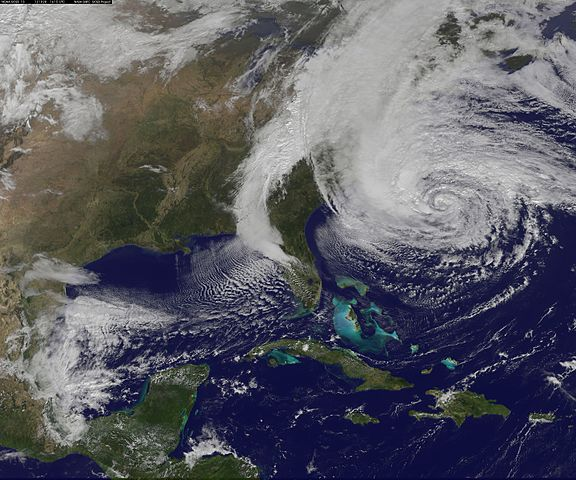
\includegraphics[width=0.8\linewidth]{images/sandy-hurricane} 

}

\caption{NASA satellite image of hurricane Sandy, 2012 (source: wikimedia commons)}\label{fig:unnamed-chunk-2}
\end{figure}

\begin{quote}
``Hurricane Sandy (unofficially referred to as Superstorm Sandy) was the
deadliest and most destructive, as well as the strongest, hurricane of the
2012 Atlantic hurricane season. Inflicting nearly \$70 billion (2012 USD) in
damage, it was the second-costliest hurricane on record in the United States
until surpassed by Hurricanes Harvey and Maria in 2017.
\end{quote}

\url{https://en.wikipedia.org/wiki/Hurricane_Sandy}

\hypertarget{a-little-bit-about-hurricanes}{%
\section{A little bit about Hurricanes}\label{a-little-bit-about-hurricanes}}

NOAA SciJinks has a webpage about basic information on hurricanes.

\url{https://scijinks.gov/hurricane/}

\begin{itemize}
\item
  Hurricanes are the most violent storms on Earth.
\item
  People call these storms by other names, such as typhoons or cyclones,
  depending on where they occur.
\item
  The scientific term for all these storms is tropical cyclone.
\item
  Only tropical cyclones that form over the Atlantic Ocean or eastern Pacific
  Ocean are called ``hurricanes.''
\item
  A tropical cyclone is a rotating low-pressure weather system that has
  organized thunderstorms but no fronts.
\item
  Hurricanes are tropical cyclones whose sustained winds have reached 74 mph.
\item
  At this point the hurricane reaches category 1 on the Saffir-Simpson
  Hurricane Wind Scale,
\item
  Saffir-Simpson Hurricane Wind Scale is a 1 to 5 rating based on a hurricane's
  sustained wind speed:

  \begin{itemize}
  \tightlist
  \item
    cateory 1: 74-95 mph; 64-82 kt; 119-153 km/h
  \item
    cateory 2: 96-110 mph; 83-95 kt; 154-177 km/h
  \item
    cateory 3: 111-129 mph; 96-112 kt; 178-208 km/h
  \item
    cateory 4: 130-156 mph; 113-136 kt; 209-251 km/h
  \item
    cateory 5: 157 mph or higher; 137 kt or higher; 252 km/h or higher
  \end{itemize}
\item
  Major hurricanes are defined as Category 3, 4, and 5 storms.
\item
  The official Atlantic hurricane season runs from June through November, but
  occasionally storms form outside those months.
\item
  September is the most active month (where most of the hurricanes occur),
  followed by August, and October (based on 1851 to 2015 data).
\item
  A typical year has 12 named storms, including six hurricanes of which three
  become major hurricanes (category 3, 4, and 5).
\item
  No hurricanes made U.S. landfall before June and after November during the period studied (1851 to 2015 data).
\end{itemize}

\hypertarget{storms}{%
\chapter{\texorpdfstring{Data Set \texttt{storms}}{Data Set storms}}\label{storms}}

In this first module, you will have your first contact with tabular data
(i.e.~data arranged in rows and columns) which is
the most common format in which data is handled for data analysis.

\hypertarget{atlantic-hurricane-data}{%
\section{Atlantic Hurricane Data}\label{atlantic-hurricane-data}}

In order to have a gentle introduction, we are going to use a data set that
comes in one the most popular R packages for manipulation of tables: \texttt{"dplyr"}.
The main reason to start in this mode, is to avoid having to worry about data
importing issues, which we cover later in the course. The other reason is to
have data that is already clean and ready to be analyzed.

\hypertarget{data-storms}{%
\subsection{\texorpdfstring{Data \texttt{storms}}{Data storms}}\label{data-storms}}

The package \texttt{"dplyr"} contains a dataset called \texttt{storms}
which is a subset of the \emph{NOAA Atlantic hurricane database best track data}.
This database is one of several data sets available in the National Hurricane
Center (NHC) Data Archive, which is part of the National Oceanic and Atmospheric
Administration (NOAA). In case you are curious about the specifications and
format of this type of data, you can visit the following link:

\url{http://www.nhc.noaa.gov/data/\#hurdat}

The data \texttt{storms} includes the positions and attributes of 198 tropical storms,
measured every six hours during the lifetime of a storm.

When you type the name of the data object, you would get something like this:

\begin{Shaded}
\begin{Highlighting}[]
\NormalTok{storms}
\end{Highlighting}
\end{Shaded}

\begin{verbatim}
## # A tibble: 11,859 x 13
##    name   year month   day  hour   lat  long status        categ~1  wind press~2
##    <chr> <dbl> <dbl> <int> <dbl> <dbl> <dbl> <chr>         <ord>   <int>   <int>
##  1 Amy    1975     6    27     0  27.5 -79   tropical dep~ -1         25    1013
##  2 Amy    1975     6    27     6  28.5 -79   tropical dep~ -1         25    1013
##  3 Amy    1975     6    27    12  29.5 -79   tropical dep~ -1         25    1013
##  4 Amy    1975     6    27    18  30.5 -79   tropical dep~ -1         25    1013
##  5 Amy    1975     6    28     0  31.5 -78.8 tropical dep~ -1         25    1012
##  6 Amy    1975     6    28     6  32.4 -78.7 tropical dep~ -1         25    1012
##  7 Amy    1975     6    28    12  33.3 -78   tropical dep~ -1         25    1011
##  8 Amy    1975     6    28    18  34   -77   tropical dep~ -1         30    1006
##  9 Amy    1975     6    29     0  34.4 -75.8 tropical sto~ 0          35    1004
## 10 Amy    1975     6    29     6  34   -74.8 tropical sto~ 0          40    1002
## # ... with 11,849 more rows, 2 more variables:
## #   tropicalstorm_force_diameter <int>, hurricane_force_diameter <int>, and
## #   abbreviated variable names 1: category, 2: pressure
\end{verbatim}

What's going on in the above output?

\begin{itemize}
\item
  \texttt{storms} is a \textbf{tibble} object, which is one of the data objects in R that
  handles data in tabular format.
\item
  tibbles are not a native R object---they come from the homonym package
  \texttt{"tibble"}---instead they are a modern version of data frames
\end{itemize}

The way tibbles are \emph{printed} is very interesting.

\begin{itemize}
\item
  the number of rows that are displayed is limited to 10;
\item
  depending on the width of the printing space, you will only see a few columns
  shown to fit such width.
\item
  underneath the name of each column there is a three letter abbreviation
  inside angle brackets
\item
  this abbreviation indicates the \emph{data type} used by R to store the values. For

  \begin{itemize}
  \tightlist
  \item
    \texttt{\textless{}chr\textgreater{}} stands for \emph{character} data
  \item
    \texttt{\textless{}dbl\textgreater{}} means \emph{double} (i.e.~real numbers or numbers with decimal digits)
  \item
    \texttt{\textless{}int\textgreater{}} means \emph{integer} (numbers with no decimal digits)
  \item
    \texttt{\textless{}ord\textgreater{}} indicates an \emph{ordinal} \texttt{factor} which is how R handles categorical
    data
  \end{itemize}
\end{itemize}

\hypertarget{storms-documentation}{%
\subsection{\texorpdfstring{\texttt{storms} Documentation}{storms Documentation}}\label{storms-documentation}}

You can find a more technical description of \texttt{storms} by taking a peek at its
manual (or help) documentation. All you need to do is run this command:

\begin{Shaded}
\begin{Highlighting}[]
\NormalTok{?storms}
\end{Highlighting}
\end{Shaded}

Take a look at the manual (or \emph{help}) documentation and find the description
of the variables in data \texttt{storms}

\hypertarget{general-inspection}{%
\section{General Inspection}\label{general-inspection}}

When dealing with a data table, especially for the first time, I like to do
a quick inspection of the \emph{general structure} of the data, meaning the number
of rows and columns, the name and data-type of each column, and some times
also to quickly inspect a few rows either at the top or at the bottom of the
table. To do all these things there is a handful of functions:

\begin{itemize}
\item
  \texttt{str()}: to get a summary of the table's structure
\item
  \texttt{dim()}: to get the dimensions (number of rows and columns)
\item
  \texttt{nrow()}: to get just the number of rows
\item
  \texttt{ncol()}: to get just the number of columns
\item
  \texttt{names()}: to get the column names; there's also \texttt{colnames()}
\item
  \texttt{head()}: to look at a few first rows
\item
  \texttt{tail()}: to look at a few last rows
\end{itemize}

Structure:

\begin{Shaded}
\begin{Highlighting}[]
\FunctionTok{str}\NormalTok{(storms, }\AttributeTok{vec.len =} \DecValTok{1}\NormalTok{)}
\end{Highlighting}
\end{Shaded}

\begin{verbatim}
## tibble [11,859 x 13] (S3: tbl_df/tbl/data.frame)
##  $ name                        : chr [1:11859] "Amy" ...
##  $ year                        : num [1:11859] 1975 ...
##  $ month                       : num [1:11859] 6 6 ...
##  $ day                         : int [1:11859] 27 27 ...
##  $ hour                        : num [1:11859] 0 6 ...
##  $ lat                         : num [1:11859] 27.5 28.5 ...
##  $ long                        : num [1:11859] -79 -79 ...
##  $ status                      : chr [1:11859] "tropical depression" ...
##  $ category                    : Ord.factor w/ 7 levels "-1"<"0"<"1"<"2"<..: 1 1 ...
##  $ wind                        : int [1:11859] 25 25 ...
##  $ pressure                    : int [1:11859] 1013 1013 ...
##  $ tropicalstorm_force_diameter: int [1:11859] NA NA ...
##  $ hurricane_force_diameter    : int [1:11859] NA NA ...
\end{verbatim}

Dimensions: number of rows and columns

\begin{Shaded}
\begin{Highlighting}[]
\FunctionTok{dim}\NormalTok{(storms)}
\FunctionTok{nrow}\NormalTok{(storms)}
\FunctionTok{ncol}\NormalTok{(storms)}
\end{Highlighting}
\end{Shaded}

\hypertarget{basic-inspection-of-year}{%
\section{\texorpdfstring{Basic Inspection of \texttt{year}}{Basic Inspection of year}}\label{basic-inspection-of-year}}

As we just saw, when you type \texttt{storms}, R displays the first 10 rows, which
belong to storm Amy in 1975:

\begin{Shaded}
\begin{Highlighting}[]
\NormalTok{storms}
\end{Highlighting}
\end{Shaded}

From this output, we know that the data contains at least one storm from 1975.
We also know, from the manual documentation of \texttt{storms}, that there
are supposed to be 198 storms. But we don't know for what years. So in a more
or less arbitrary way, let's begin inspecting \texttt{storms} by focusing on column
\texttt{year}. Our first exploratory question is:

\begin{quote}
\textbf{What years have the data been collected for?}
\end{quote}

There are several ways in R to manipulate a column from a tabular object. Using
\texttt{"dplyr"}, there are two basic kinds of functions to extract variables:
\texttt{pull()} and \texttt{select()}.

\begin{figure}

{\centering 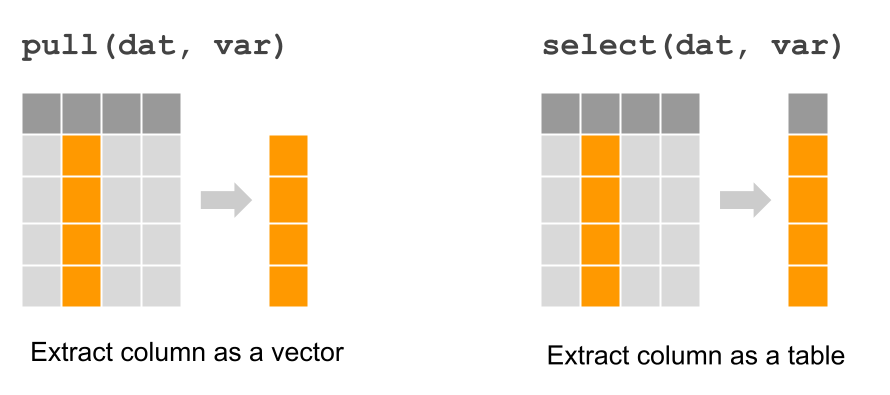
\includegraphics[width=0.65\linewidth]{images/dplyr-extract-column} 

}

\caption{Extracting a column with dplyr functions "pull" and "select"}\label{fig:unnamed-chunk-9}
\end{figure}

Let's do a sanity check of years. We can use the function \texttt{pull()} that \emph{pulls}
or extracts an entire column. Because there are 10010 elements in
\texttt{years}, let's also use \texttt{unique()} to find out the set of year values in the
data. First we pull the year, and then we identify unique occurrences:

\begin{Shaded}
\begin{Highlighting}[]
\FunctionTok{unique}\NormalTok{(}\FunctionTok{pull}\NormalTok{(storms, year))}
\end{Highlighting}
\end{Shaded}

\begin{verbatim}
##  [1] 1975 1976 1977 1978 1979 1980 1981 1982 1983 1984 1985 1986 1987 1988 1989
## [16] 1990 1991 1992 1993 1994 1995 1996 1997 1998 1999 2000 2001 2002 2003 2004
## [31] 2005 2006 2007 2008 2009 2010 2011 2012 2013 2014 2015 2016 2017 2018 2019
## [46] 2020
\end{verbatim}

The same can be accomplished with \texttt{select()}. The difference with \texttt{pull()} is
in the way the output is handled by \texttt{select()}, which returns output in a table
format:

\begin{Shaded}
\begin{Highlighting}[]
\FunctionTok{unique}\NormalTok{(}\FunctionTok{select}\NormalTok{(storms, year))}
\end{Highlighting}
\end{Shaded}

\begin{verbatim}
## # A tibble: 46 x 1
##     year
##    <dbl>
##  1  1975
##  2  1976
##  3  1977
##  4  1978
##  5  1979
##  6  1980
##  7  1981
##  8  1982
##  9  1983
## 10  1984
## # ... with 36 more rows
\end{verbatim}

Based on the previous answers, we can see that \texttt{storms} has records during
a 41-year period since 1975 to 2015.

\hypertarget{barplot-of-year-values}{%
\subsection{\texorpdfstring{Barplot of \texttt{year} values}{Barplot of year values}}\label{barplot-of-year-values}}

Let's keep using the values in column \texttt{year} to obtain our first visualization
with \texttt{"ggplot2"} functions. You could certainly begin a visual exploration of
other variables, but we think \texttt{year} is a good place to start because it's a
numeric variable, measured on a discrete scale, and this is a good candidate
to use barcharts (the most popular type of graphic).

\texttt{"ggplot2"} comes with a large number of functions to create almost any
type of chart. Luckily for us, it already comes with predefined
functions to graph barcharts. The syntax may seem a bit scary for beginners,
but you will see that it follows a logical structure. Here's the code to make
a barplot of values in \texttt{year}:

\begin{Shaded}
\begin{Highlighting}[]
\CommentTok{\# barchart of year values}
\FunctionTok{ggplot}\NormalTok{(}\AttributeTok{data =}\NormalTok{ storms) }\SpecialCharTok{+} 
  \FunctionTok{geom\_bar}\NormalTok{(}\FunctionTok{aes}\NormalTok{(}\AttributeTok{x =}\NormalTok{ year))}
\end{Highlighting}
\end{Shaded}

\begin{center}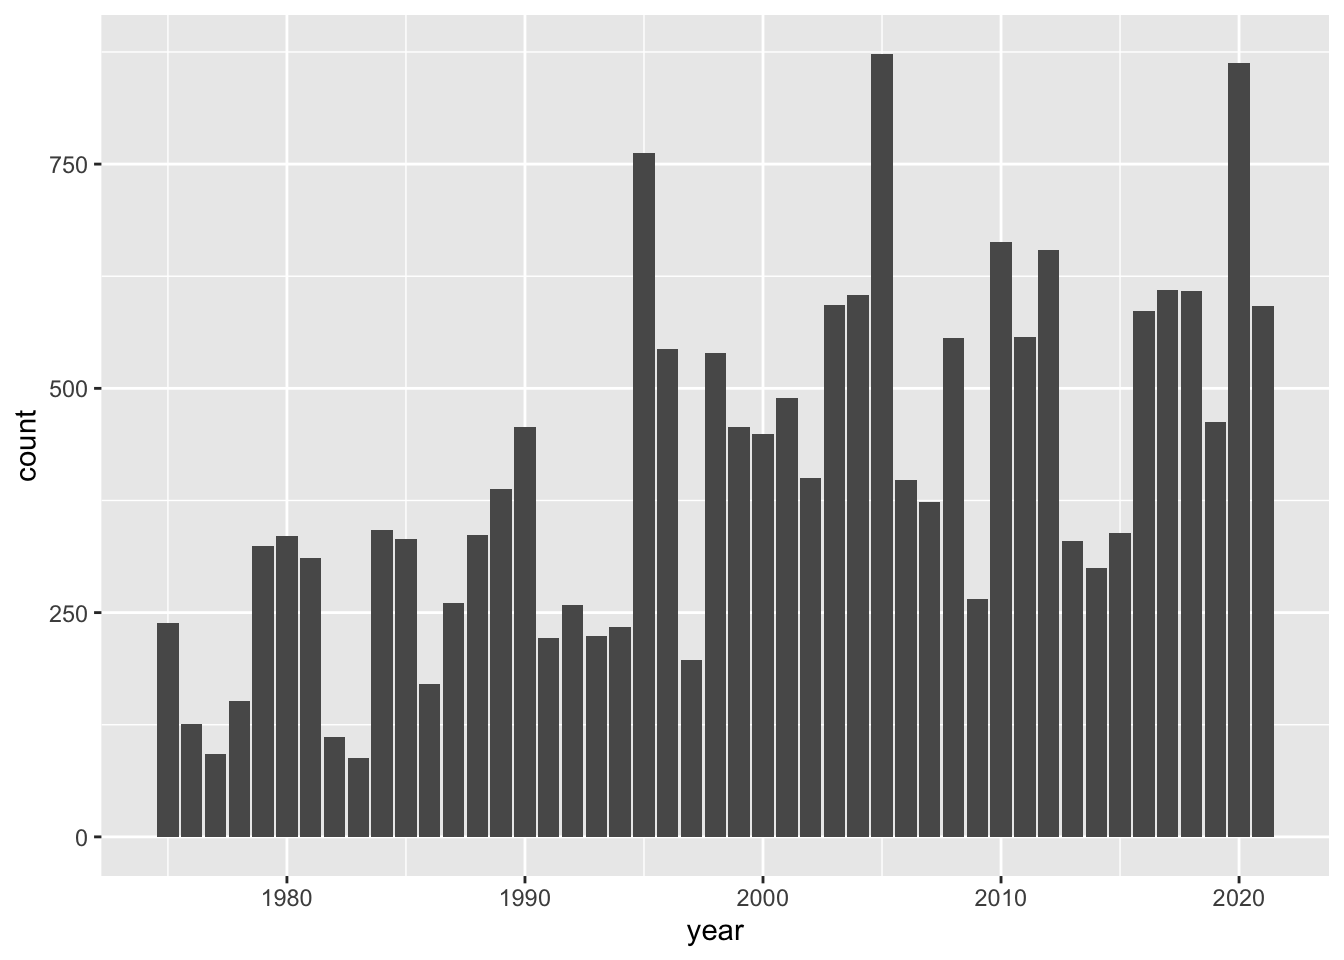
\includegraphics{R-tidy-hurricanes_files/figure-latex/plot-barchart-year-1} \end{center}

How does the previous command work?

\begin{itemize}
\item
  First, we always call the \texttt{ggplot()} function, typically indicating the name
  of the table to be used with the \texttt{data} argument.
\item
  Then, we add more components, or \textbf{layers}, using the plus \texttt{+} operator.
\item
  In this case we are adding just one layer: a \texttt{geom\_bar()} component which is
  the geometric object for bars.
\item
  To tell \texttt{ggplot()} that \texttt{year} is the column in \texttt{data\ =\ storms} to be used for
  the x-axis, we \textbf{map} \texttt{x\ =\ year} inside the \texttt{aes()} function which stands for
  \emph{aesthetic} mapping.
\end{itemize}

We should clarify that the meaning of ``aesthetic'' as used by \texttt{"ggplot2"} does
not mean beautiful or pretty, instead it conserves its etymological
meaning of \emph{perception}. Simply put, \texttt{aes()} is the function that you use to
tell \texttt{ggplot()} which variables of a \texttt{data} object will be mapped as visual
attributes of graphical elements.

\begin{center}\rule{0.5\linewidth}{0.5pt}\end{center}

\hypertarget{your-turn}{%
\section{Your Turn}\label{your-turn}}

\begin{itemize}
\item
  Use \texttt{pull()}, \texttt{select()}, and \texttt{unique()} to inspect the values in column
  \texttt{month}
\item
  Try to use \texttt{sort()} in order to arrange the unique values of \texttt{month}
\item
  Does the unique month values make sense? Are there months for which there
  seem to be no recorded storm data?
\item
  Use \texttt{"ggplot2"} functions to graph a barchart for the values in column
  \texttt{month}.
\item
  Look at the cheatsheet for ggplot and locate the information for \texttt{geom\_bar()}.
  Find out how to specify: border \texttt{color}, \texttt{fill} color. Also, see what happens
  when you specify \texttt{alpha\ =\ 0.5}.
\item
  Look at the cheatsheet for ggplot and locate the information for background
  \emph{Themes}, e.g.~\texttt{theme\_bw()}. Find out how to add theme \texttt{theme\_classic()} to the
  previous barchart.
\item
  Look at the cheatsheet for ggplot and locate the information for \emph{Labels}.
  Find out how to add a title with \texttt{ggtitle()} as well as with \texttt{labs()} to one
  of your previous barcharts.
\item
  Create a barchart of \texttt{month} values. Does the plot make sense?
\end{itemize}

\hypertarget{part-analyzing-storms-in-1975}{%
\part{Analyzing Storms in 1975}\label{part-analyzing-storms-in-1975}}

\hypertarget{storms-in-1975}{%
\chapter{Storms in 1975}\label{storms-in-1975}}

Let's focus on those storms recorded in 1975. How do we select them?
Computationally, this operation involves a logical condition: \texttt{year\ ==\ 1975}.
This condition means that, from all the available year values, we get those
that match 1975. This is done via \texttt{"dplyr"} function \texttt{filter()}

\begin{figure}

{\centering 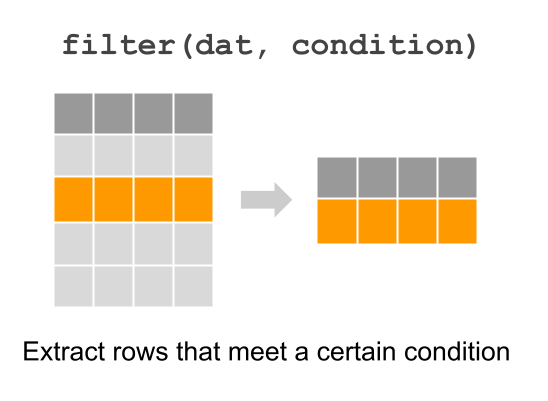
\includegraphics[width=0.4\linewidth]{images/dplyr-filter} 

}

\caption{Extracting a row with dplyr function "filter"}\label{fig:unnamed-chunk-12}
\end{figure}

First, let's create a subset \texttt{storms75} by \emph{filtering} those rows with \texttt{year}
equal to 1975:

\begin{Shaded}
\begin{Highlighting}[]
\NormalTok{storms75 }\OtherTok{\textless{}{-}} \FunctionTok{filter}\NormalTok{(storms, year }\SpecialCharTok{==} \DecValTok{1975}\NormalTok{)}
\NormalTok{storms75}
\end{Highlighting}
\end{Shaded}

\begin{verbatim}
## # A tibble: 86 x 13
##    name   year month   day  hour   lat  long status        categ~1  wind press~2
##    <chr> <dbl> <dbl> <int> <dbl> <dbl> <dbl> <chr>         <ord>   <int>   <int>
##  1 Amy    1975     6    27     0  27.5 -79   tropical dep~ -1         25    1013
##  2 Amy    1975     6    27     6  28.5 -79   tropical dep~ -1         25    1013
##  3 Amy    1975     6    27    12  29.5 -79   tropical dep~ -1         25    1013
##  4 Amy    1975     6    27    18  30.5 -79   tropical dep~ -1         25    1013
##  5 Amy    1975     6    28     0  31.5 -78.8 tropical dep~ -1         25    1012
##  6 Amy    1975     6    28     6  32.4 -78.7 tropical dep~ -1         25    1012
##  7 Amy    1975     6    28    12  33.3 -78   tropical dep~ -1         25    1011
##  8 Amy    1975     6    28    18  34   -77   tropical dep~ -1         30    1006
##  9 Amy    1975     6    29     0  34.4 -75.8 tropical sto~ 0          35    1004
## 10 Amy    1975     6    29     6  34   -74.8 tropical sto~ 0          40    1002
## # ... with 76 more rows, 2 more variables: tropicalstorm_force_diameter <int>,
## #   hurricane_force_diameter <int>, and abbreviated variable names 1: category,
## #   2: pressure
\end{verbatim}

Once we have the set of storms that occurred in 1975, one possible question
to ask is what \texttt{unique()} storms happened in that year:

\begin{Shaded}
\begin{Highlighting}[]
\FunctionTok{unique}\NormalTok{(}\FunctionTok{pull}\NormalTok{(storms75, name))}
\end{Highlighting}
\end{Shaded}

\begin{verbatim}
## [1] "Amy"      "Caroline" "Doris"
\end{verbatim}

From the returned output, there are only three unique storms recorded in 1975.

A similar result can be obtained with \texttt{distinct()}, the difference being the
way in which the output is returned, in this case under the format of a tibble:

\begin{Shaded}
\begin{Highlighting}[]
\FunctionTok{distinct}\NormalTok{(storms75, name)}
\end{Highlighting}
\end{Shaded}

\begin{verbatim}
## # A tibble: 3 x 1
##   name    
##   <chr>   
## 1 Amy     
## 2 Caroline
## 3 Doris
\end{verbatim}

Now that we know there are three storms for 1975, it would be nice to count
the number of rows or records for each of them. \texttt{"dplyr"} allows us to do this
with \texttt{count()}, passing the name of the table, and then the name of the column
for which we want to get the counts or frequencies:

\begin{Shaded}
\begin{Highlighting}[]
\FunctionTok{count}\NormalTok{(storms75, name)}
\end{Highlighting}
\end{Shaded}

\begin{verbatim}
## # A tibble: 3 x 2
##   name         n
##   <chr>    <int>
## 1 Amy         30
## 2 Caroline    33
## 3 Doris       23
\end{verbatim}

\hypertarget{visualizing-1975-data}{%
\section{Visualizing 1975 data}\label{visualizing-1975-data}}

Let's play a bit with those storms from 1975. More specifically, let's visually
explore the values of columns \texttt{wind} and \texttt{pressure}.

\begin{Shaded}
\begin{Highlighting}[]
\NormalTok{storms75}
\end{Highlighting}
\end{Shaded}

\begin{verbatim}
## # A tibble: 86 x 13
##    name   year month   day  hour   lat  long status        categ~1  wind press~2
##    <chr> <dbl> <dbl> <int> <dbl> <dbl> <dbl> <chr>         <ord>   <int>   <int>
##  1 Amy    1975     6    27     0  27.5 -79   tropical dep~ -1         25    1013
##  2 Amy    1975     6    27     6  28.5 -79   tropical dep~ -1         25    1013
##  3 Amy    1975     6    27    12  29.5 -79   tropical dep~ -1         25    1013
##  4 Amy    1975     6    27    18  30.5 -79   tropical dep~ -1         25    1013
##  5 Amy    1975     6    28     0  31.5 -78.8 tropical dep~ -1         25    1012
##  6 Amy    1975     6    28     6  32.4 -78.7 tropical dep~ -1         25    1012
##  7 Amy    1975     6    28    12  33.3 -78   tropical dep~ -1         25    1011
##  8 Amy    1975     6    28    18  34   -77   tropical dep~ -1         30    1006
##  9 Amy    1975     6    29     0  34.4 -75.8 tropical sto~ 0          35    1004
## 10 Amy    1975     6    29     6  34   -74.8 tropical sto~ 0          40    1002
## # ... with 76 more rows, 2 more variables: tropicalstorm_force_diameter <int>,
## #   hurricane_force_diameter <int>, and abbreviated variable names 1: category,
## #   2: pressure
\end{verbatim}

What type of visual display can we use to graph \texttt{wind} speed? The answer to
this question is based by determining which type of variable \texttt{wind} is.
You would agree with us in saying that \texttt{wind} is a quantitative variable. So
one graphing option can be either a histogram or a boxplot, which are
statistical charts to visualize the distribution of quantitative variables.

\hypertarget{histograms}{%
\subsection{Histograms}\label{histograms}}

Let's begin with a histogram. The associated \texttt{geom\_()} function to plot a
histogram is \texttt{geom\_histogram()}. We are going to show you a synatx of
\texttt{ggplot()} slightly different from the one we used for the barcharts.
Carefully review the following code:

\begin{Shaded}
\begin{Highlighting}[]
\FunctionTok{ggplot}\NormalTok{(}\AttributeTok{data =}\NormalTok{ storms75, }\FunctionTok{aes}\NormalTok{(}\AttributeTok{x =}\NormalTok{ wind)) }\SpecialCharTok{+}
  \FunctionTok{geom\_histogram}\NormalTok{()}
\end{Highlighting}
\end{Shaded}

\begin{verbatim}
## `stat_bin()` using `bins = 30`. Pick better value with `binwidth`.
\end{verbatim}

\begin{center}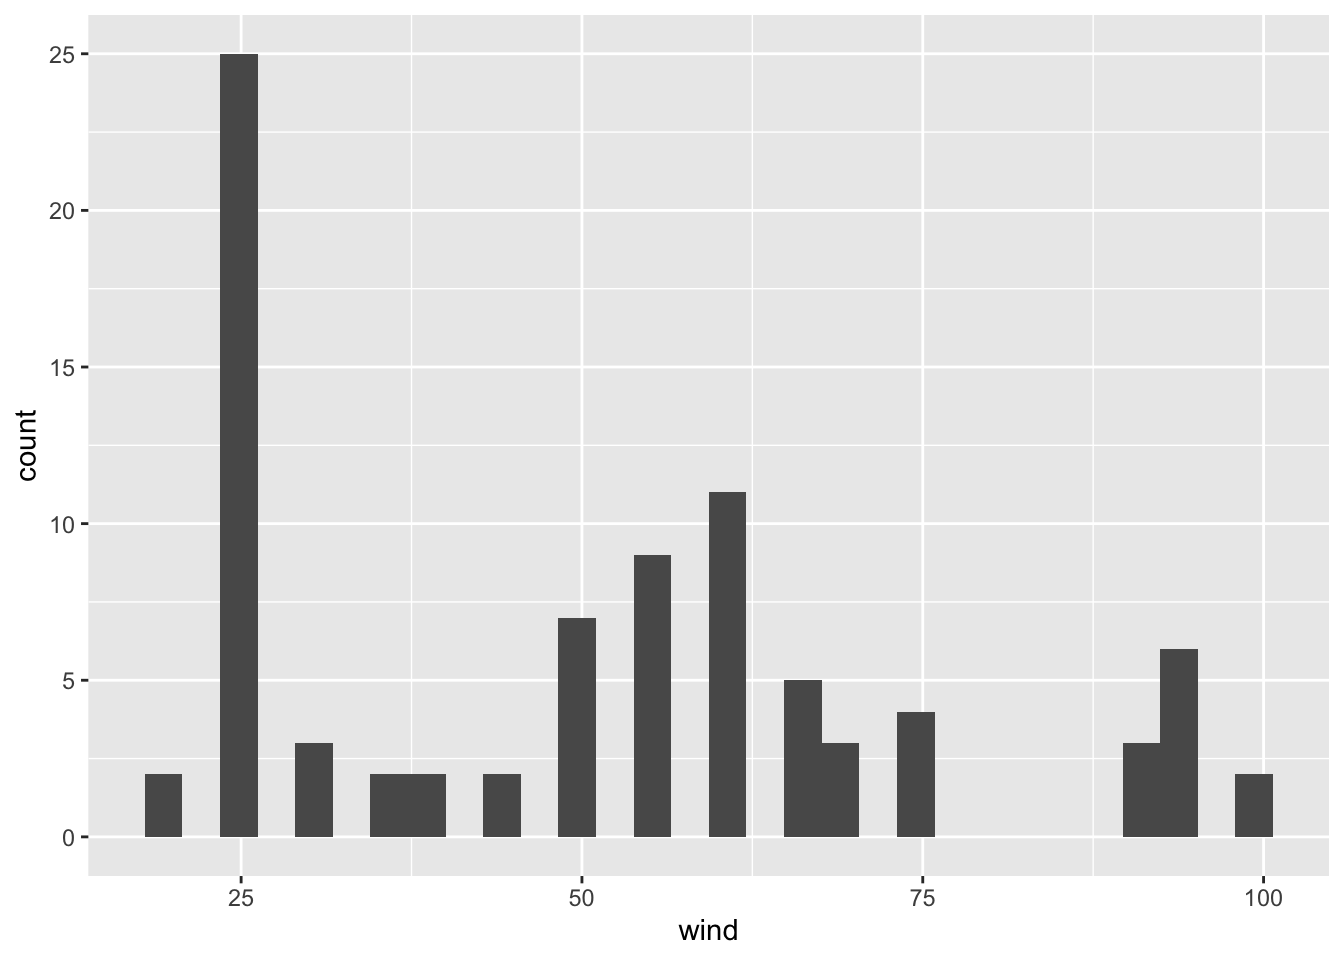
\includegraphics[width=0.7\linewidth]{R-tidy-hurricanes_files/figure-latex/plot-hist1-wind75-1} \end{center}

You should notice now that \texttt{aes()} is an argument of \texttt{ggplot()}, and not anymore
an argument of the geometric-object function \texttt{geom\_histogram()}. While this
may be a bit confusing when learning about \texttt{"ggplot2"}, it is a very flexible
and powerful behavior of \texttt{aes()}. Again, the important part of \texttt{aes()} is to
understand that this function allows you to tell \texttt{ggplot()} which variables
in your \texttt{data} table are used as visual attributes of the corresponding
geometric elements forming the plot.

We can change the default argument \texttt{binwidth} to get another version of the
histogram, for example a bin-width of 5 units (i.e.~width of 5 knots):

\begin{Shaded}
\begin{Highlighting}[]
\FunctionTok{ggplot}\NormalTok{(}\AttributeTok{data =}\NormalTok{ storms75, }\FunctionTok{aes}\NormalTok{(}\AttributeTok{x =}\NormalTok{ wind)) }\SpecialCharTok{+}
  \FunctionTok{geom\_histogram}\NormalTok{(}\AttributeTok{binwidth =} \DecValTok{5}\NormalTok{)}
\end{Highlighting}
\end{Shaded}

\begin{center}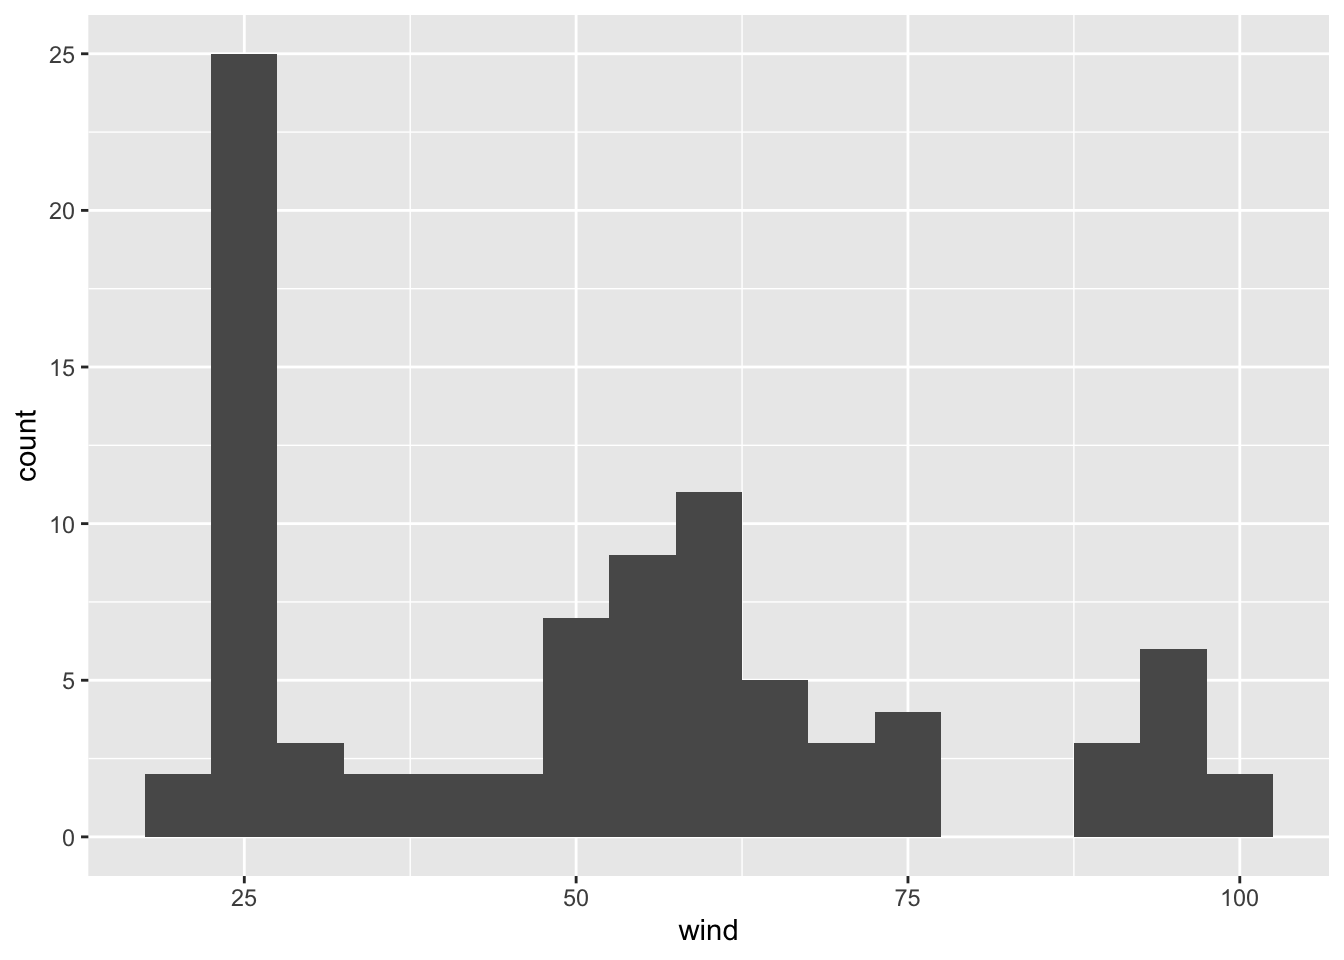
\includegraphics[width=0.7\linewidth]{R-tidy-hurricanes_files/figure-latex/plot-hist2-wind75-1} \end{center}

or a bin-width of 10:

\begin{Shaded}
\begin{Highlighting}[]
\FunctionTok{ggplot}\NormalTok{(}\AttributeTok{data =}\NormalTok{ storms75, }\FunctionTok{aes}\NormalTok{(}\AttributeTok{x =}\NormalTok{ wind)) }\SpecialCharTok{+}
  \FunctionTok{geom\_histogram}\NormalTok{(}\AttributeTok{binwidth =} \DecValTok{10}\NormalTok{)}
\end{Highlighting}
\end{Shaded}

\begin{center}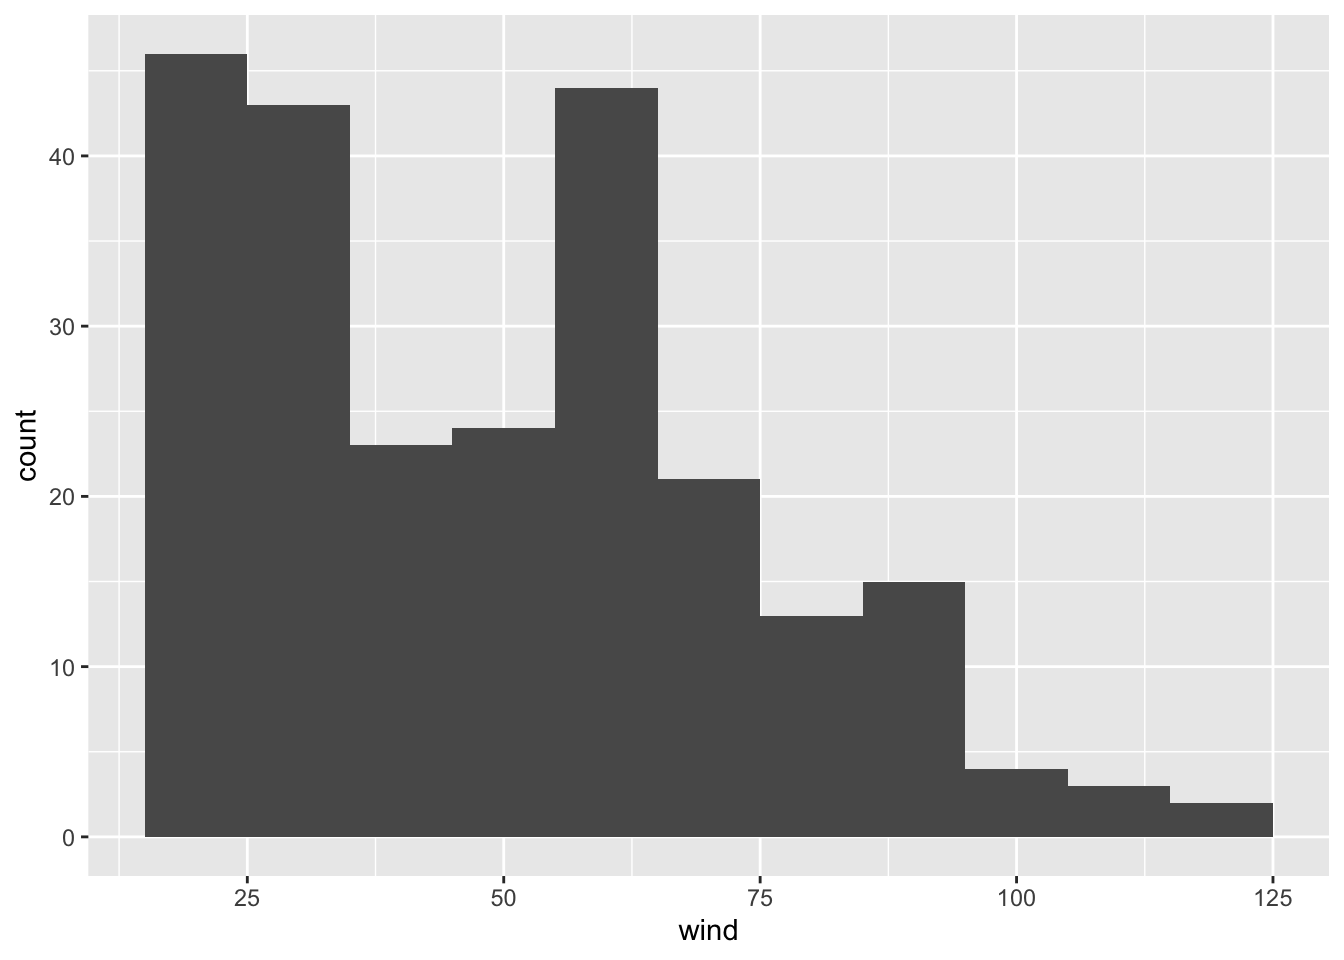
\includegraphics[width=0.7\linewidth]{R-tidy-hurricanes_files/figure-latex/plot-hist3-wind75-1} \end{center}

Now, let's reflect on what's going on in each of the histograms. Do they make
sense? How do we interpret each figure?

\hypertarget{boxplots}{%
\subsection{Boxplots}\label{boxplots}}

While \texttt{ggplot()} does what we ask it to do, the displays may not be the most
useful, or meaningful. Why? Think what exactly it is that we are plotting.
In 1975, there are three storms:

\begin{Shaded}
\begin{Highlighting}[]
\FunctionTok{unique}\NormalTok{(}\FunctionTok{pull}\NormalTok{(storms75, name))}
\end{Highlighting}
\end{Shaded}

\begin{verbatim}
## [1] "Amy"      "Caroline" "Doris"
\end{verbatim}

But the histograms are not differentiating between any of those three storms.
Rather, the visualization is just giving us a general view of the \texttt{wind} values,
from the low 20's to the high 90's, or to be more precise:

\begin{Shaded}
\begin{Highlighting}[]
\FunctionTok{summary}\NormalTok{(}\FunctionTok{pull}\NormalTok{(storms75, wind))}
\end{Highlighting}
\end{Shaded}

\begin{verbatim}
##    Min. 1st Qu.  Median    Mean 3rd Qu.    Max. 
##   20.00   25.00   52.50   50.87   65.00  100.00
\end{verbatim}

However, we don't really know if all three storms have the same minimum \texttt{wind}
speed, or the same maximum \texttt{wind} speed. The good news is that we can tell
\texttt{ggplot()} to take into account each different storm name. But now let's use
boxplots via \texttt{geom\_boxplot()}, mapping \texttt{name} to the x-axis, and \texttt{wind} to the y-axis.

\begin{Shaded}
\begin{Highlighting}[]
\FunctionTok{ggplot}\NormalTok{(}\AttributeTok{data =}\NormalTok{ storms75, }\FunctionTok{aes}\NormalTok{(}\AttributeTok{x =}\NormalTok{ name, }\AttributeTok{y =}\NormalTok{ wind)) }\SpecialCharTok{+}
  \FunctionTok{geom\_boxplot}\NormalTok{()}
\end{Highlighting}
\end{Shaded}

\begin{center}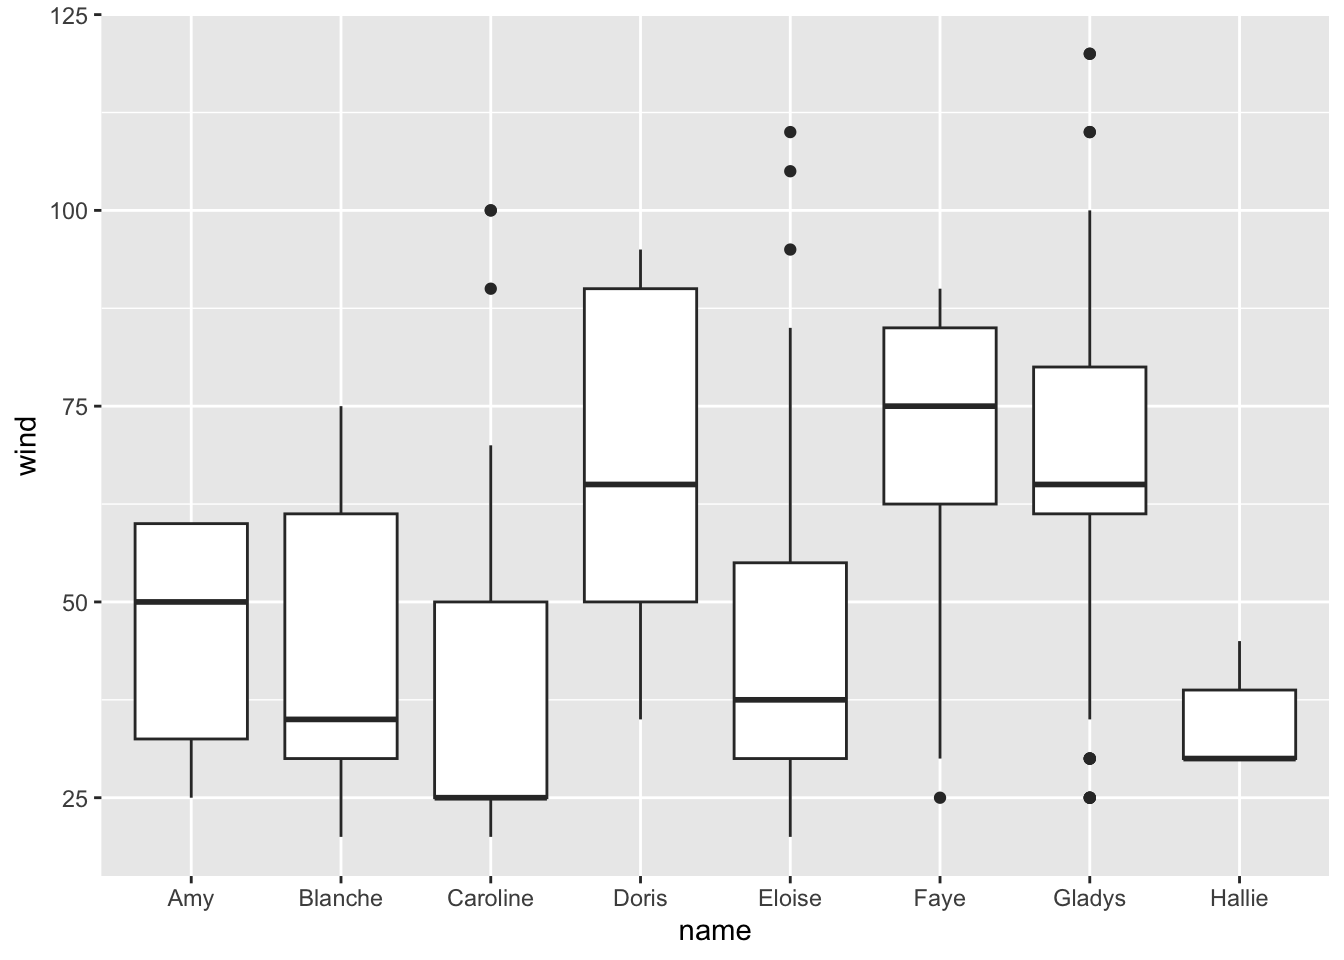
\includegraphics[width=0.7\linewidth]{R-tidy-hurricanes_files/figure-latex/plot-box-wind75-1} \end{center}

Note how different the distribution of wind speed is in each storm. We can get
an alternative plot with density curves thanks to the \texttt{geom\_density()} function.
The syntax in this case is different. Let's first do it without separating
storms, and then we do it taking into account the storm names.

\hypertarget{density-curves}{%
\subsection{Density Curves}\label{density-curves}}

Here's the command that plots a density curve of wind, without distinguishing
between storms. Observe also how the argument \texttt{fill} is \emph{set} to color \texttt{\textquotesingle{}gray\textquotesingle{}}:

\begin{Shaded}
\begin{Highlighting}[]
\FunctionTok{ggplot}\NormalTok{(}\AttributeTok{data =}\NormalTok{ storms75, }\FunctionTok{aes}\NormalTok{(}\AttributeTok{x =}\NormalTok{ wind)) }\SpecialCharTok{+}
  \FunctionTok{geom\_density}\NormalTok{(}\AttributeTok{fill =} \StringTok{\textquotesingle{}gray\textquotesingle{}}\NormalTok{)}
\end{Highlighting}
\end{Shaded}

\begin{center}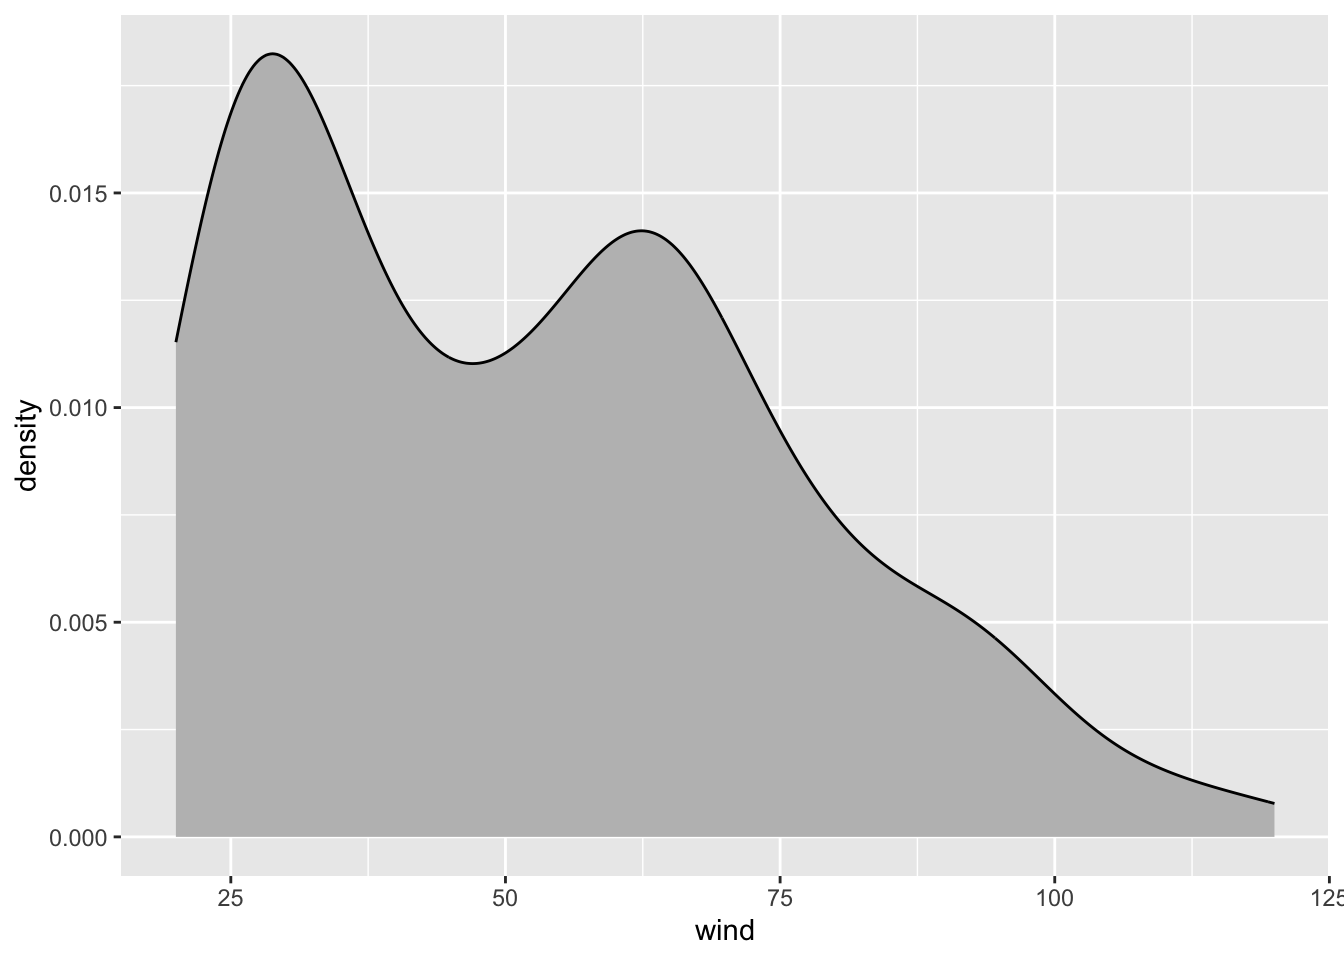
\includegraphics[width=0.7\linewidth]{R-tidy-hurricanes_files/figure-latex/plot-density1-wind75-1} \end{center}

As you can tell, the density curve looks like the profile of a roller coaster,
or like the silhouette of three mountain peaks. Is this a pattern followed
by wind speed in all storms? Or is it just an artifact due to the fact that we
are plotting data without taking into consideration the context of \texttt{storms75}?

Let's replot density of wind, but now distinguishing between each storm. We
do this by mapping \texttt{name} to the \texttt{color} argument:

\begin{Shaded}
\begin{Highlighting}[]
\FunctionTok{ggplot}\NormalTok{(}\AttributeTok{data =}\NormalTok{ storms75, }\FunctionTok{aes}\NormalTok{(}\AttributeTok{x =}\NormalTok{ wind, }\AttributeTok{color =}\NormalTok{ name)) }\SpecialCharTok{+}
  \FunctionTok{geom\_density}\NormalTok{(}\FunctionTok{aes}\NormalTok{(}\AttributeTok{fill =}\NormalTok{ name))}
\end{Highlighting}
\end{Shaded}

\begin{center}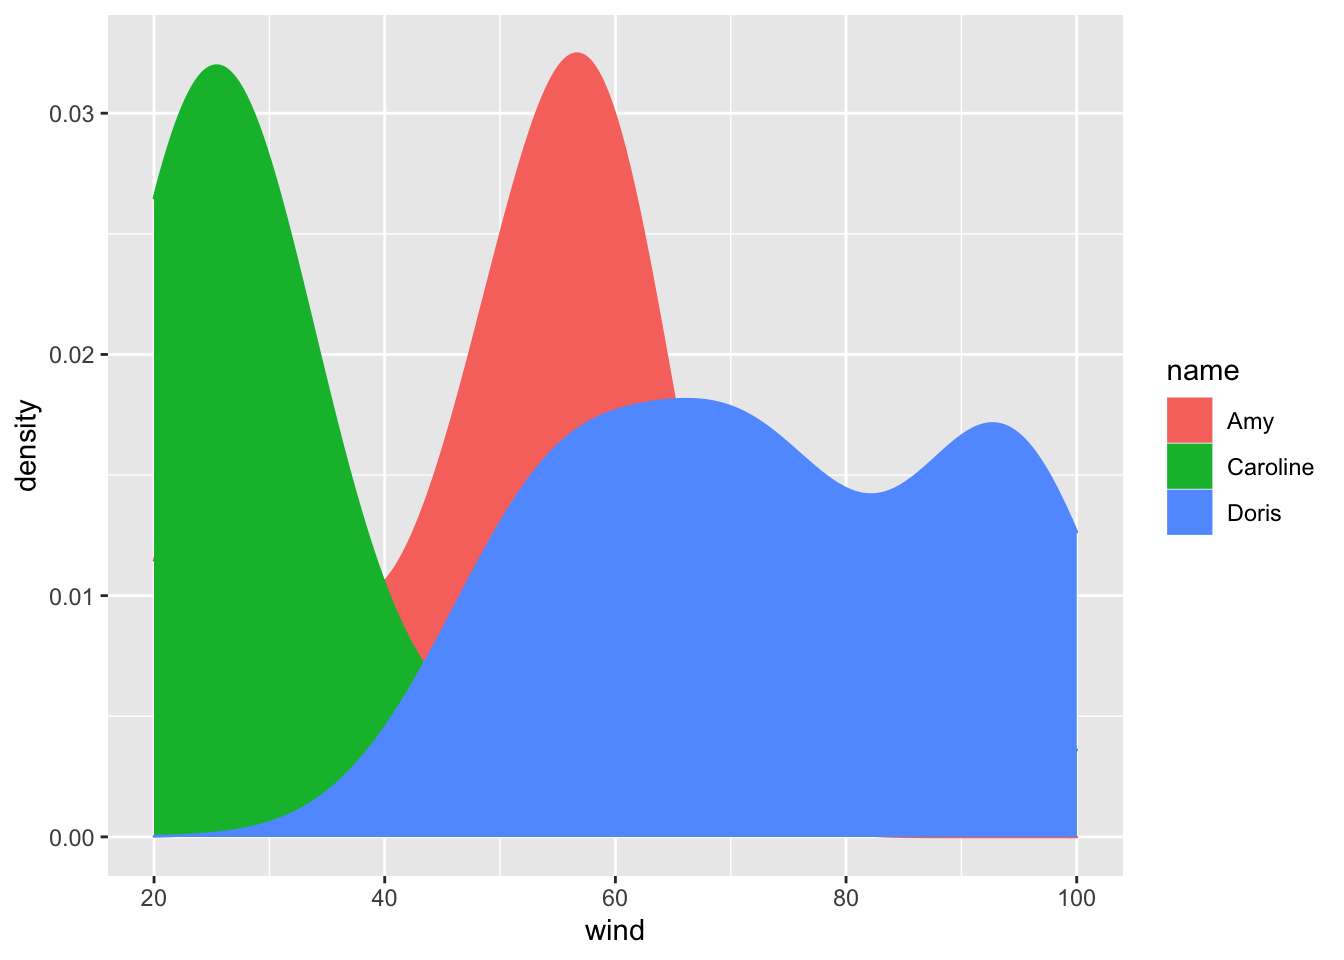
\includegraphics[width=0.7\linewidth]{R-tidy-hurricanes_files/figure-latex/plot-density2-wind75-1} \end{center}

Aha! Now things look more interesting: the roller coast shape of the first call
to \texttt{geom\_density()} turned out to be an artificial pattern. As you can tell
from the above plot, each storm has its own different density curve.

To get a better visualization, we can take the previous command and add a bit
of transparency to the colors, this is done with the argument \texttt{alpha} inside
\texttt{geom\_density()}. Note how arguments are specified inside \texttt{geom\_density()}:
we \textbf{map} \texttt{name} to the color-fill attribute of the curve inside \texttt{aes()}, but
we \textbf{set} \texttt{alpha\ =\ 0.5} outside \texttt{aes()}:

\begin{Shaded}
\begin{Highlighting}[]
\FunctionTok{ggplot}\NormalTok{(}\AttributeTok{data =}\NormalTok{ storms75, }\FunctionTok{aes}\NormalTok{(}\AttributeTok{x =}\NormalTok{ wind, }\AttributeTok{color =}\NormalTok{ name)) }\SpecialCharTok{+}
  \FunctionTok{geom\_density}\NormalTok{(}\FunctionTok{aes}\NormalTok{(}\AttributeTok{fill =}\NormalTok{ name), }\AttributeTok{alpha =} \FloatTok{0.5}\NormalTok{)}
\end{Highlighting}
\end{Shaded}

\begin{center}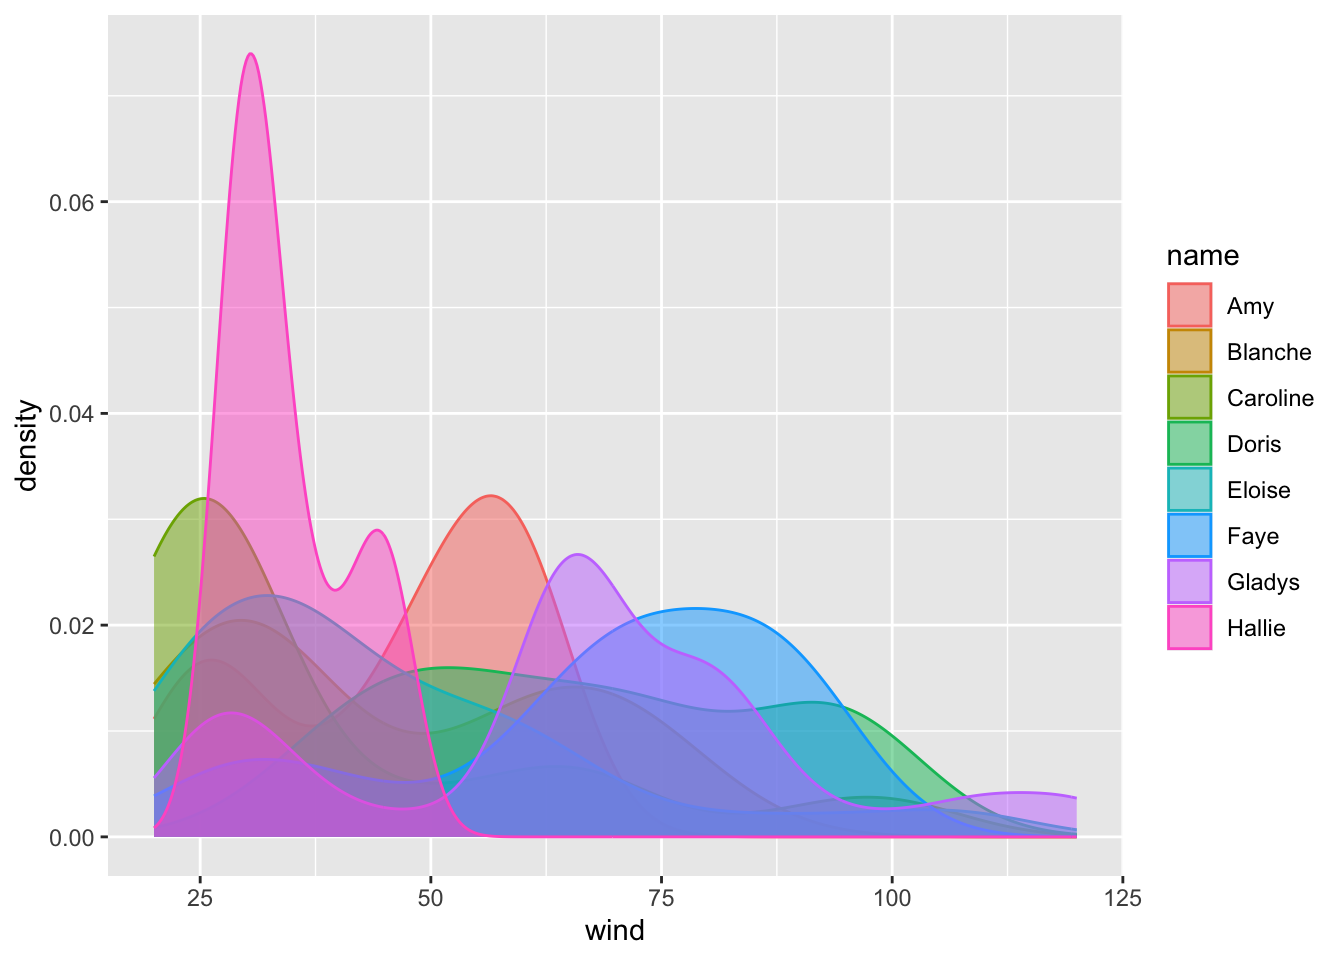
\includegraphics[width=0.7\linewidth]{R-tidy-hurricanes_files/figure-latex/plot-density3-wind75-1} \end{center}

\hypertarget{facets}{%
\subsection{Facets}\label{facets}}

We are going to take advantage of this graphic to introduce another cool
feature of \texttt{"ggplot2"} that allows us to split data based on categorical or
discrete variables, in order to produce separated frames called \textbf{facets}.
Here's the previous command---without \texttt{alpha} transparency---adding a
new layer given by \texttt{facet\_wrap()} taking into account the \texttt{name} of the
storms:

\begin{Shaded}
\begin{Highlighting}[]
\FunctionTok{ggplot}\NormalTok{(}\AttributeTok{data =}\NormalTok{ storms75, }\FunctionTok{aes}\NormalTok{(}\AttributeTok{x =}\NormalTok{ wind, }\AttributeTok{color =}\NormalTok{ name)) }\SpecialCharTok{+}
  \FunctionTok{geom\_density}\NormalTok{(}\FunctionTok{aes}\NormalTok{(}\AttributeTok{fill =}\NormalTok{ name)) }\SpecialCharTok{+} 
  \FunctionTok{facet\_wrap}\NormalTok{(}\SpecialCharTok{\textasciitilde{}}\NormalTok{ name)}
\end{Highlighting}
\end{Shaded}

\begin{center}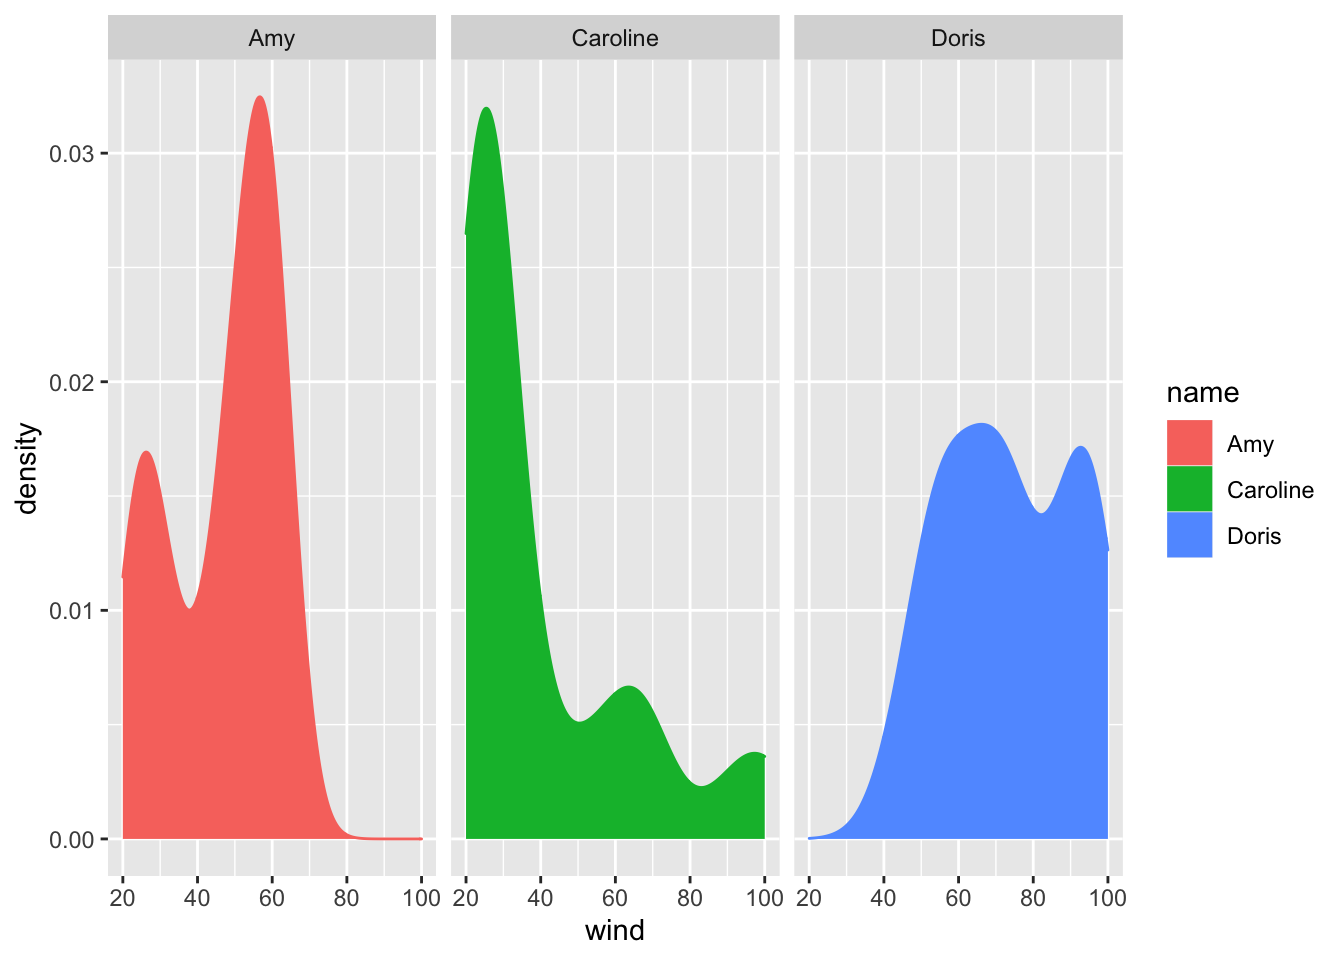
\includegraphics[width=0.7\linewidth]{R-tidy-hurricanes_files/figure-latex/plot-density4-wind75-1} \end{center}

In this command we are faceting by \texttt{name}. We obtain a facet for each unique
category of \texttt{name}. In other words, we get separated density curves, one for
each storm. The syntax inside \texttt{facet\_wrap()} uses the tilde \texttt{\textasciitilde{}} operator which
is the \emph{formula} operator in R. Basically, the command \texttt{\textasciitilde{}\ name} tells
\texttt{ggplot()} to create facets based on the values of \texttt{name}.

\hypertarget{storm-amy-1975}{%
\chapter{Storm Amy (1975)}\label{storm-amy-1975}}

Let's focus on storm \texttt{Amy} in 1975, subsetting \texttt{storms75} to filter out just
the rows of Amy into its own table

\begin{Shaded}
\begin{Highlighting}[]
\NormalTok{amy75 }\OtherTok{\textless{}{-}} \FunctionTok{filter}\NormalTok{(storms75, name }\SpecialCharTok{==} \StringTok{"Amy"}\NormalTok{)}
\NormalTok{amy75}
\end{Highlighting}
\end{Shaded}

\begin{verbatim}
## # A tibble: 30 x 13
##    name   year month   day  hour   lat  long status        categ~1  wind press~2
##    <chr> <dbl> <dbl> <int> <dbl> <dbl> <dbl> <chr>         <ord>   <int>   <int>
##  1 Amy    1975     6    27     0  27.5 -79   tropical dep~ -1         25    1013
##  2 Amy    1975     6    27     6  28.5 -79   tropical dep~ -1         25    1013
##  3 Amy    1975     6    27    12  29.5 -79   tropical dep~ -1         25    1013
##  4 Amy    1975     6    27    18  30.5 -79   tropical dep~ -1         25    1013
##  5 Amy    1975     6    28     0  31.5 -78.8 tropical dep~ -1         25    1012
##  6 Amy    1975     6    28     6  32.4 -78.7 tropical dep~ -1         25    1012
##  7 Amy    1975     6    28    12  33.3 -78   tropical dep~ -1         25    1011
##  8 Amy    1975     6    28    18  34   -77   tropical dep~ -1         30    1006
##  9 Amy    1975     6    29     0  34.4 -75.8 tropical sto~ 0          35    1004
## 10 Amy    1975     6    29     6  34   -74.8 tropical sto~ 0          40    1002
## # ... with 20 more rows, 2 more variables: tropicalstorm_force_diameter <int>,
## #   hurricane_force_diameter <int>, and abbreviated variable names 1: category,
## #   2: pressure
\end{verbatim}

\hypertarget{exploring-wind}{%
\section{\texorpdfstring{Exploring \texttt{wind}}{Exploring wind}}\label{exploring-wind}}

Let's keep exploring \texttt{wind} but now let's do it chronologically, that is,
graphing the wind values in the order that they were recorded (recall storms
are tracked every six hours).

We begin with a scatterplot using \texttt{geom\_point()},
and we specify that the x-axis should use a numeric sequence \texttt{1:nrow(amy75)}
from the first row till the last row of \texttt{amy75}, and \texttt{wind} for y-axis:

\begin{Shaded}
\begin{Highlighting}[]
\FunctionTok{ggplot}\NormalTok{(}\AttributeTok{data =}\NormalTok{ amy75, }\FunctionTok{aes}\NormalTok{(}\AttributeTok{x =} \DecValTok{1}\SpecialCharTok{:}\FunctionTok{nrow}\NormalTok{(amy75), }\AttributeTok{y =}\NormalTok{ wind)) }\SpecialCharTok{+}
  \FunctionTok{geom\_point}\NormalTok{()}
\end{Highlighting}
\end{Shaded}

\begin{center}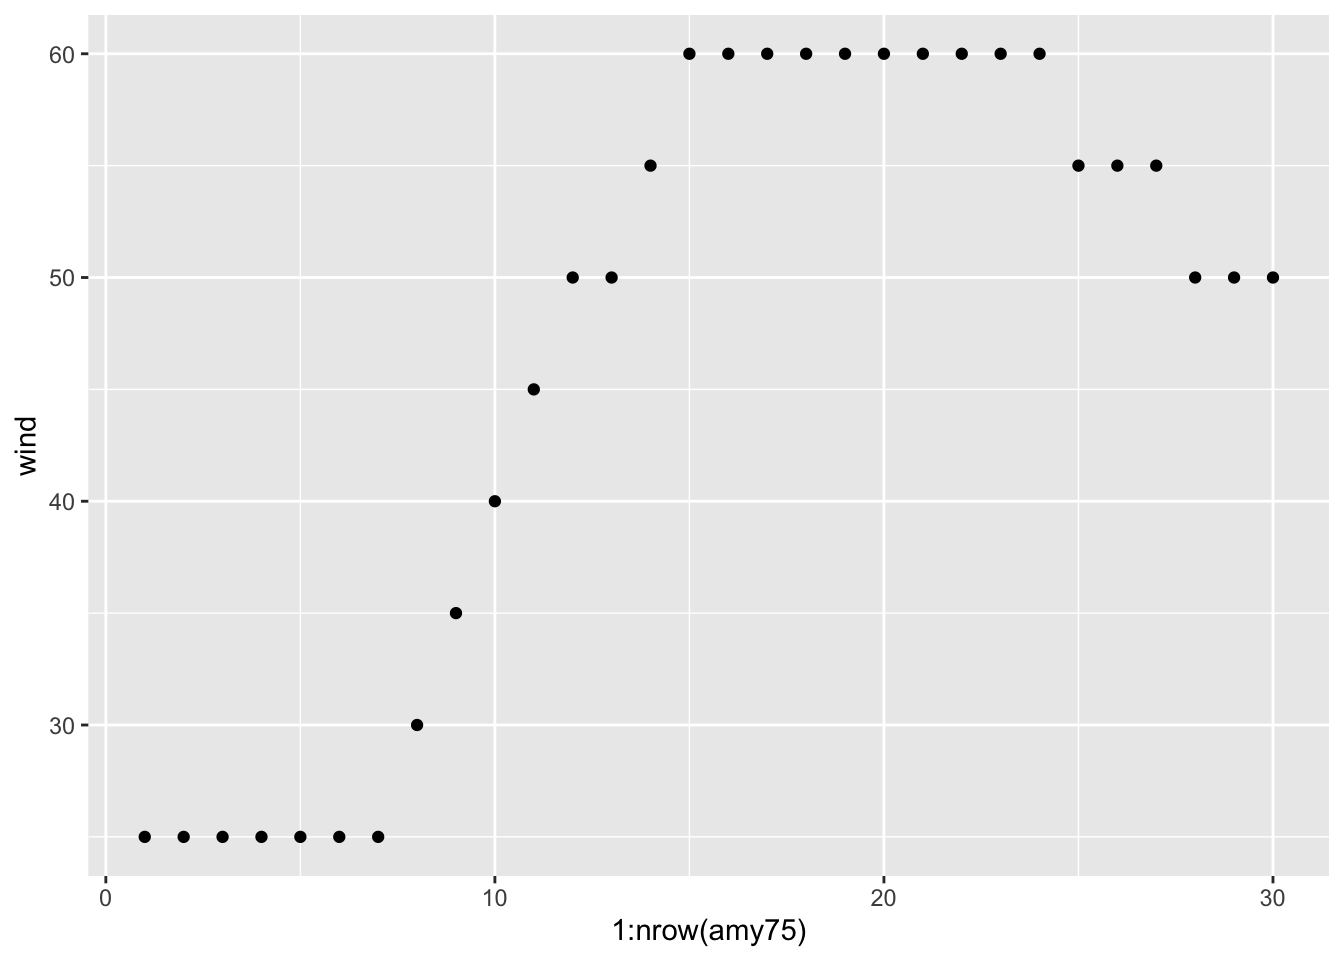
\includegraphics[width=0.8\linewidth]{R-tidy-hurricanes_files/figure-latex/plot-scatter1-amy75-wind-1} \end{center}

Because the x-axis denotes progression over time, we can connect the dots
with a line. A simple way to do this is by adding another layer to our plot,
this time with \texttt{geom\_line()}

\begin{Shaded}
\begin{Highlighting}[]
\FunctionTok{ggplot}\NormalTok{(}\AttributeTok{data =}\NormalTok{ amy75, }\FunctionTok{aes}\NormalTok{(}\AttributeTok{x =} \DecValTok{1}\SpecialCharTok{:}\FunctionTok{nrow}\NormalTok{(amy75), }\AttributeTok{y =}\NormalTok{ wind)) }\SpecialCharTok{+}
  \FunctionTok{geom\_point}\NormalTok{() }\SpecialCharTok{+} 
  \FunctionTok{geom\_line}\NormalTok{()}
\end{Highlighting}
\end{Shaded}

\begin{center}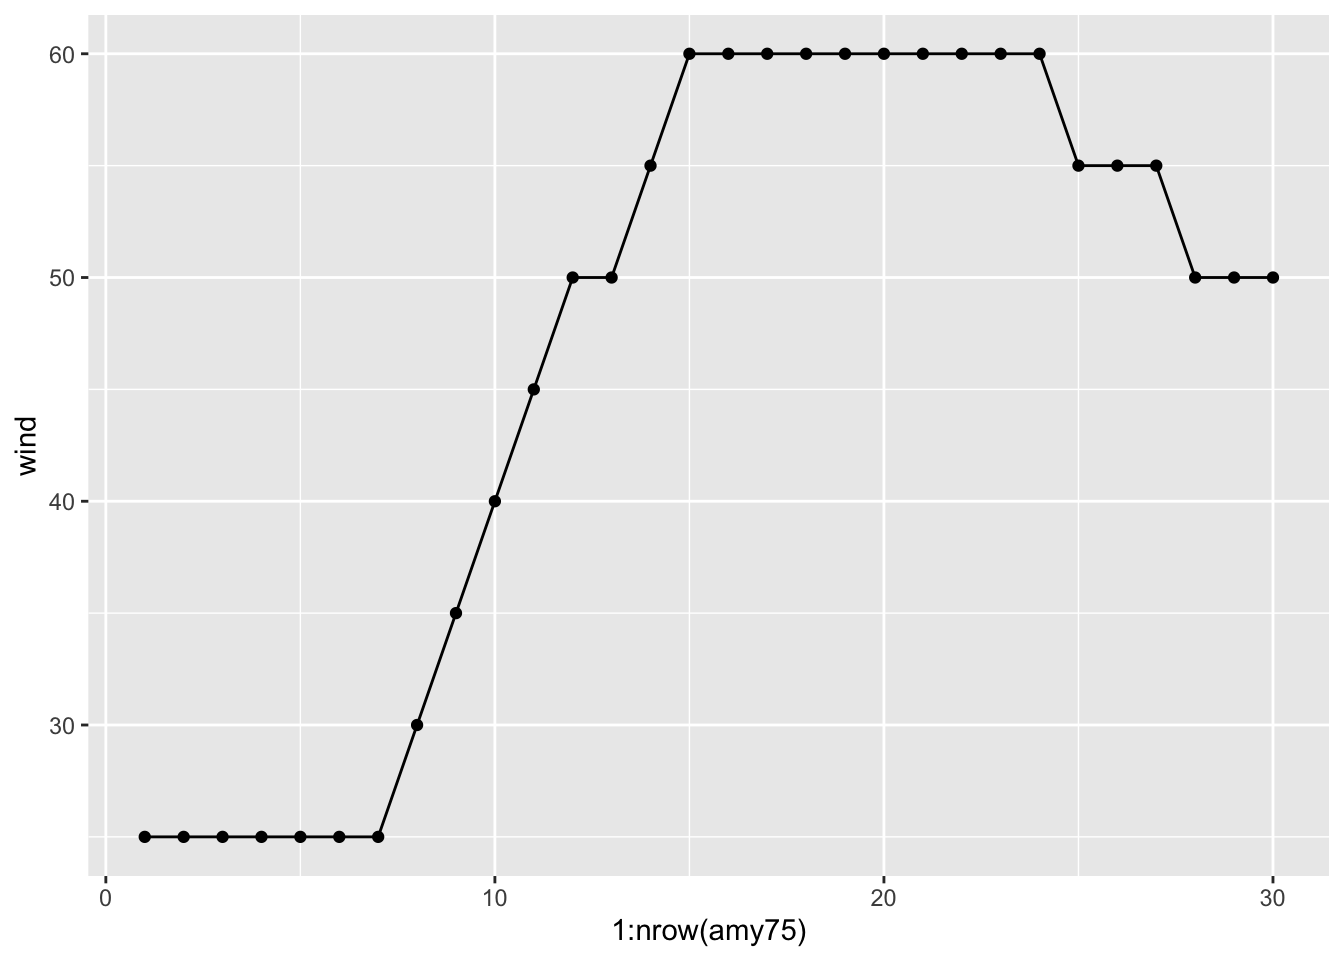
\includegraphics[width=0.8\linewidth]{R-tidy-hurricanes_files/figure-latex/plot-scatter2-amy75-wind-1} \end{center}

As you can tell, Amy started to being recorded with wind speed of 25 knots, and
then after (7 x 6) = 42 hours, its speed kept increasing to 30, 35, 40, and so on
until reaching its maximum speed of 60 knots that lasted 54 hours (9 x 6).

At this point, we can ask about the \texttt{status} of Amy along its lifetime. One
option is to map \texttt{status} to the \texttt{color} attribute of points:

\begin{Shaded}
\begin{Highlighting}[]
\FunctionTok{ggplot}\NormalTok{(}\AttributeTok{data =}\NormalTok{ amy75, }\FunctionTok{aes}\NormalTok{(}\AttributeTok{x =} \DecValTok{1}\SpecialCharTok{:}\FunctionTok{nrow}\NormalTok{(amy75), }\AttributeTok{y =}\NormalTok{ wind)) }\SpecialCharTok{+}
  \FunctionTok{geom\_point}\NormalTok{(}\FunctionTok{aes}\NormalTok{(}\AttributeTok{color =}\NormalTok{ status)) }\SpecialCharTok{+} 
  \FunctionTok{geom\_line}\NormalTok{()}
\end{Highlighting}
\end{Shaded}

\begin{center}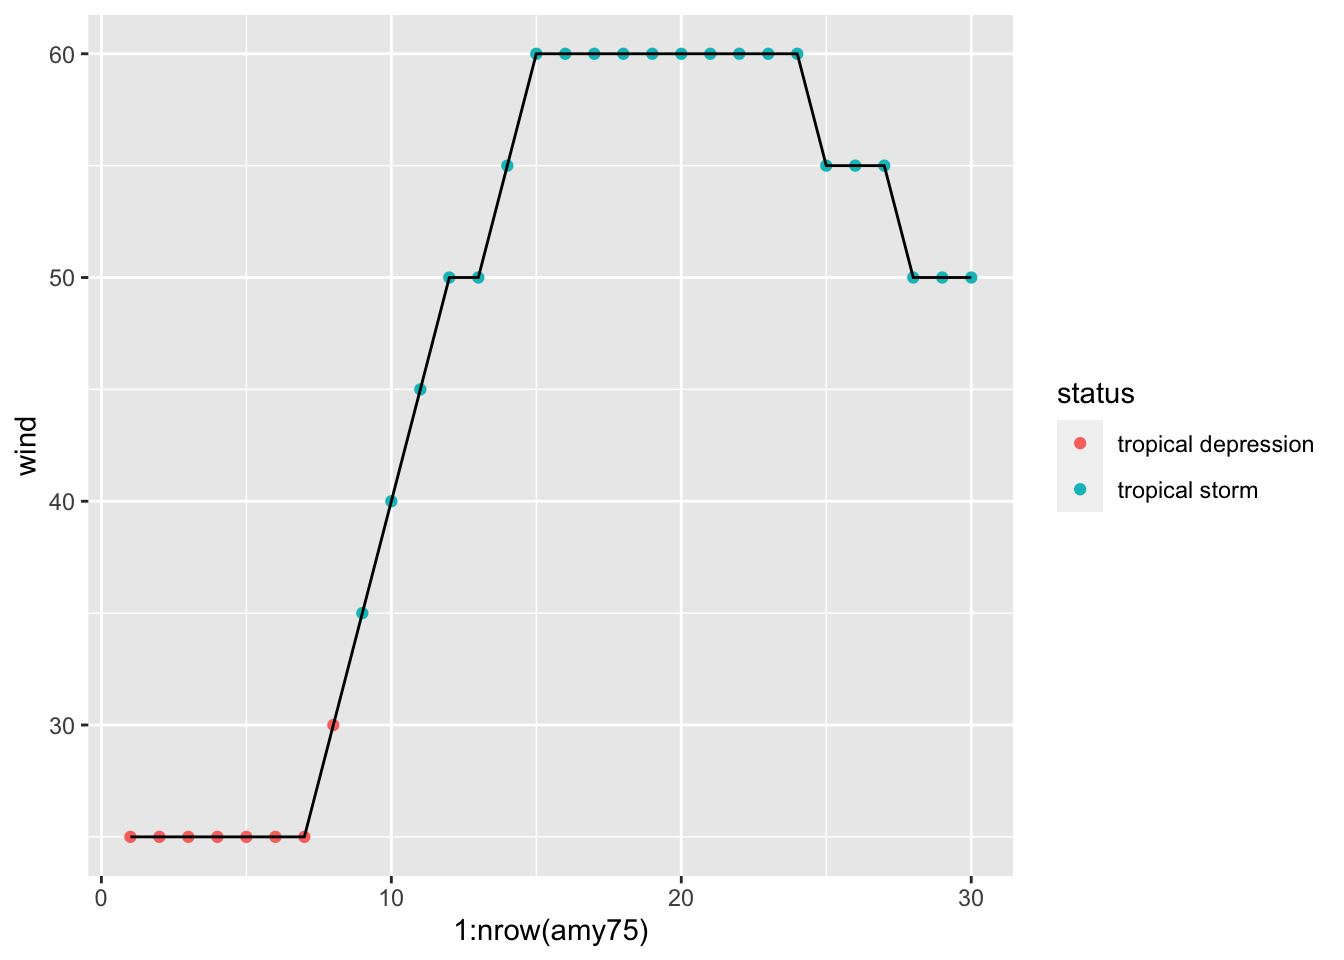
\includegraphics[width=0.8\linewidth]{R-tidy-hurricanes_files/figure-latex/plot-scatter3-amy75-wind-1} \end{center}

We see that Amy started as a tropical depression, and then became a tropical
storm, but never became a hurricane. For a storm to reach hurricane status, of category 1, it must have one-minute maximum sustained winds of at least 64 kn
(33 m/s; 74 mph; 119 km/h).

\hypertarget{exploring-pressure}{%
\section{\texorpdfstring{Exploring \texttt{pressure}}{Exploring pressure}}\label{exploring-pressure}}

What about the pressure values of Amy? We can produce a similar scatterplot
with a line connecting the dots:

\begin{Shaded}
\begin{Highlighting}[]
\FunctionTok{ggplot}\NormalTok{(}\AttributeTok{data =}\NormalTok{ amy75, }\FunctionTok{aes}\NormalTok{(}\AttributeTok{x =} \DecValTok{1}\SpecialCharTok{:}\FunctionTok{nrow}\NormalTok{(amy75), }\AttributeTok{y =}\NormalTok{ pressure)) }\SpecialCharTok{+}
  \FunctionTok{geom\_point}\NormalTok{(}\FunctionTok{aes}\NormalTok{(}\AttributeTok{color =}\NormalTok{ status)) }\SpecialCharTok{+} 
  \FunctionTok{geom\_line}\NormalTok{()}
\end{Highlighting}
\end{Shaded}

\begin{center}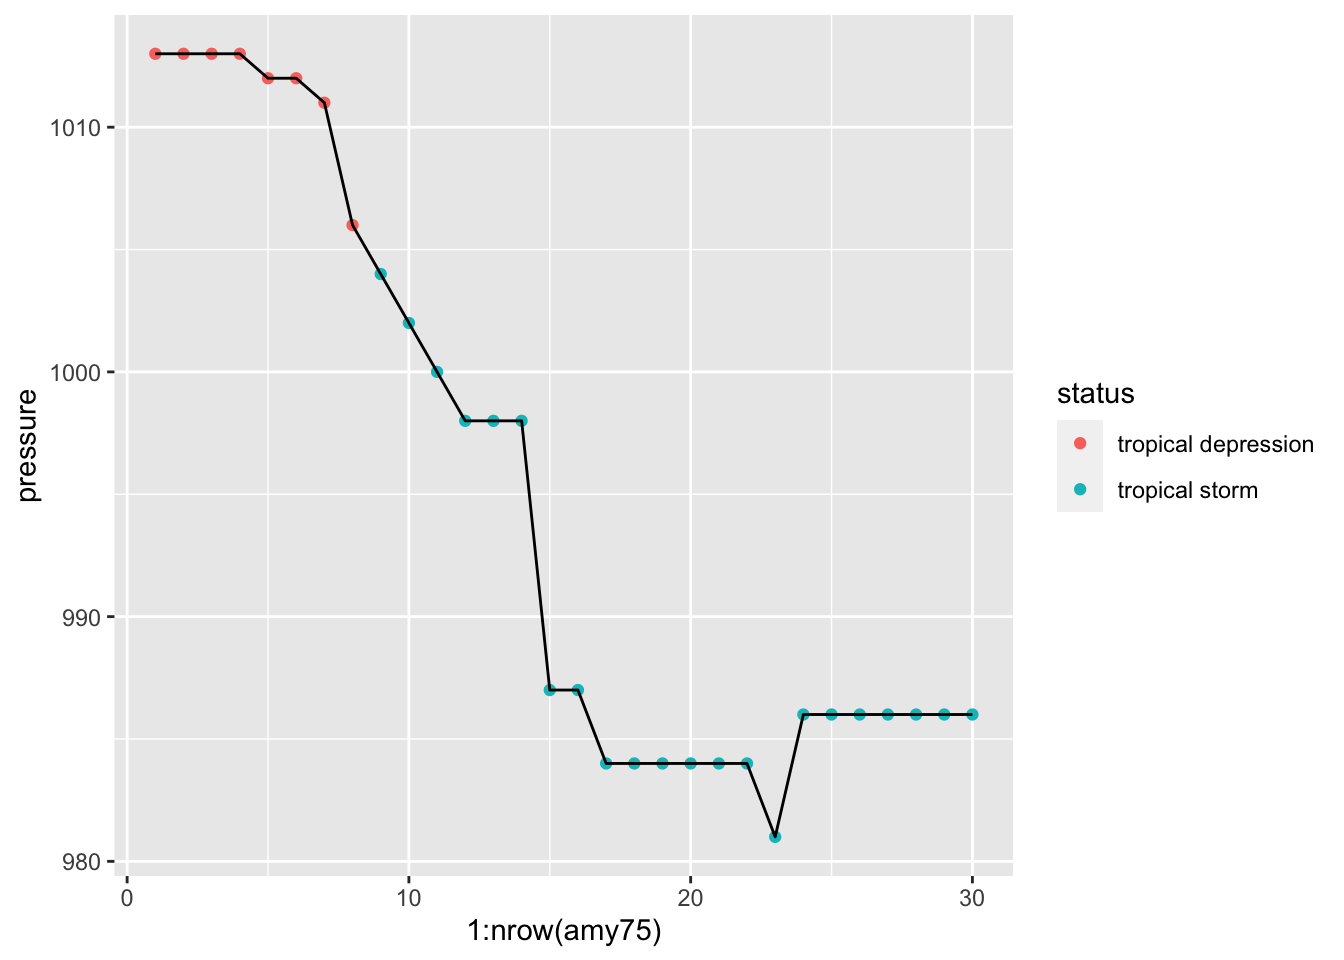
\includegraphics[width=0.8\linewidth]{R-tidy-hurricanes_files/figure-latex/plot-scatter1-amy75-press-1} \end{center}

As an exploratory exercise, we can also play with the size of points, the
size (width) of lines, colors, etc. Here's one suggestion graphing \texttt{pressure}
and taking into account the \texttt{wind} speed reflected in the size of points and
line segments:

\begin{Shaded}
\begin{Highlighting}[]
\FunctionTok{ggplot}\NormalTok{(}\AttributeTok{data =}\NormalTok{ amy75, }\FunctionTok{aes}\NormalTok{(}\AttributeTok{x =} \DecValTok{1}\SpecialCharTok{:}\FunctionTok{nrow}\NormalTok{(amy75), }\AttributeTok{y =}\NormalTok{ pressure)) }\SpecialCharTok{+}
  \FunctionTok{geom\_line}\NormalTok{(}\FunctionTok{aes}\NormalTok{(}\AttributeTok{size =}\NormalTok{ wind), }\AttributeTok{lineend =} \StringTok{"round"}\NormalTok{, }\AttributeTok{color =} \StringTok{\textquotesingle{}gray70\textquotesingle{}}\NormalTok{) }\SpecialCharTok{+}
  \FunctionTok{geom\_point}\NormalTok{(}\FunctionTok{aes}\NormalTok{(}\AttributeTok{size =}\NormalTok{ wind, }\AttributeTok{color =}\NormalTok{ status))}
\end{Highlighting}
\end{Shaded}

\begin{center}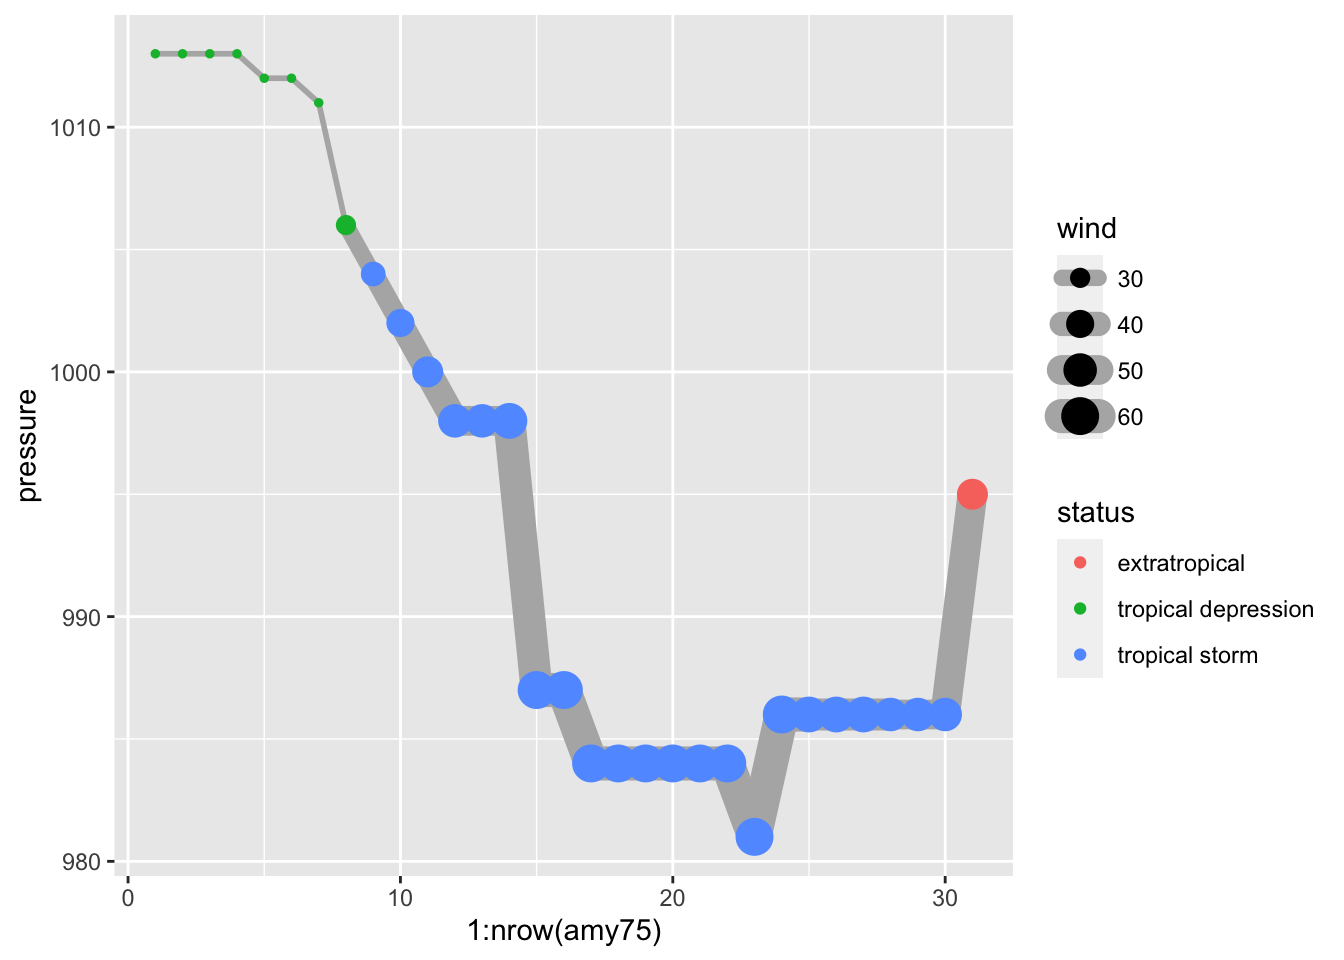
\includegraphics[width=0.8\linewidth]{R-tidy-hurricanes_files/figure-latex/plot-scatter2-amy75-press-1} \end{center}

If you know a little bit about storms, you know that there's actually an
association between \texttt{wind} and \texttt{pressure}. But let's pretend for a second that
we don't know much about tropical storms, hurricanes, and things like that.
By looking at the previous chart, this should allows us to guess that something
is going on between the \texttt{pressure} of a storm and its \texttt{wind} speed. As Amy
becomes stronger, with higher winds, its pressure levels drop accordingly,
suggesting a negative correlation, which is confirmed when we compute this
statistic:

\begin{Shaded}
\begin{Highlighting}[]
\FunctionTok{summarise}\NormalTok{(amy75, }\FunctionTok{cor}\NormalTok{(wind, pressure))}
\end{Highlighting}
\end{Shaded}

\begin{verbatim}
## # A tibble: 1 x 1
##   `cor(wind, pressure)`
##                   <dbl>
## 1                -0.956
\end{verbatim}

\begin{center}\rule{0.5\linewidth}{0.5pt}\end{center}

\hypertarget{your-turn-1}{%
\section{Your Turn}\label{your-turn-1}}

\begin{itemize}
\item
  Repeat the previous exploratory steps but now with storms from year 1980.
\item
  Try to find out how to specify a logical condition to filter various years:
  for example, storms from years 1975, 1976, and 1977.
\item
  Try to find out how to specify a logical condition to filter storms from
  year 1975 with \texttt{wind} values less than 100.
\item
  Use \texttt{"dplyr"} functions/commands to create a table (e.g.~tibble)
  \texttt{storm\_names\_1980s} containing the name and year of storms recorded during the
  1980s (i.e.~from 1980 to 1989).
\item
  Create boxplots of pressure, for storms in 1980. You can also try
  graphing \emph{violins} (\texttt{geom\_violin()}) instead of boxplots (\texttt{geom\_boxplot()}).
\item
  Use \texttt{"ggplot2"} functions to make a single scatterplot of \texttt{wind} and
  \texttt{pressure} for all storms. Use \texttt{category} to add color to the dots.
\item
  Use \texttt{"ggplot2"} functions to make a scatterplot of \texttt{wind} and \texttt{pressure}
  for all storms, facetting by month, and using \texttt{category} to differentiate by
  color.
\item
  Use \texttt{"ggplot2"} functions to make a scatterplot of \texttt{wind} and \texttt{pressure}
  for all storms, but now create facets based on \texttt{month}. Feel free to add
  some amount of \texttt{alpha} transparency to the color of dots.
\end{itemize}

\hypertarget{summarizing-1975-data}{%
\chapter{Summarizing 1975 Data}\label{summarizing-1975-data}}

We've been working with the table \texttt{storms75}, which was obtained by \emph{filtering}
those rows with \texttt{year} equal to 1975:

\begin{Shaded}
\begin{Highlighting}[]
\NormalTok{storms75 }\OtherTok{\textless{}{-}} \FunctionTok{filter}\NormalTok{(storms, year }\SpecialCharTok{==} \DecValTok{1975}\NormalTok{)}
\NormalTok{storms75}
\end{Highlighting}
\end{Shaded}

\begin{verbatim}
## # A tibble: 86 x 13
##    name   year month   day  hour   lat  long status        categ~1  wind press~2
##    <chr> <dbl> <dbl> <int> <dbl> <dbl> <dbl> <chr>         <ord>   <int>   <int>
##  1 Amy    1975     6    27     0  27.5 -79   tropical dep~ -1         25    1013
##  2 Amy    1975     6    27     6  28.5 -79   tropical dep~ -1         25    1013
##  3 Amy    1975     6    27    12  29.5 -79   tropical dep~ -1         25    1013
##  4 Amy    1975     6    27    18  30.5 -79   tropical dep~ -1         25    1013
##  5 Amy    1975     6    28     0  31.5 -78.8 tropical dep~ -1         25    1012
##  6 Amy    1975     6    28     6  32.4 -78.7 tropical dep~ -1         25    1012
##  7 Amy    1975     6    28    12  33.3 -78   tropical dep~ -1         25    1011
##  8 Amy    1975     6    28    18  34   -77   tropical dep~ -1         30    1006
##  9 Amy    1975     6    29     0  34.4 -75.8 tropical sto~ 0          35    1004
## 10 Amy    1975     6    29     6  34   -74.8 tropical sto~ 0          40    1002
## # ... with 76 more rows, 2 more variables: tropicalstorm_force_diameter <int>,
## #   hurricane_force_diameter <int>, and abbreviated variable names 1: category,
## #   2: pressure
\end{verbatim}

\hypertarget{group-by-operations}{%
\section{Group-by Operations}\label{group-by-operations}}

Another common task when exploring data has to do with computations applied
on certain groups or categories of data. \texttt{"dplyr"} provides the function
\texttt{group\_by()} which takes a data table, and we specify the column(s) on which
rows will be grouped by:

\begin{figure}

{\centering 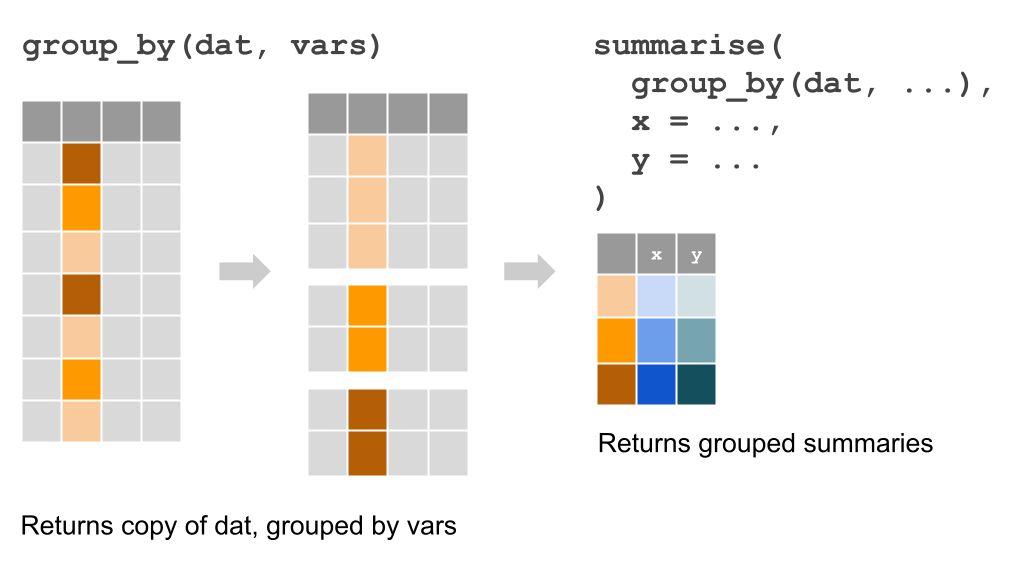
\includegraphics[width=0.8\linewidth]{images/dplyr-group-by} 

}

\caption{Group-by operations}\label{fig:unnamed-chunk-23}
\end{figure}

For example, we may be interested in calculating the average \texttt{wind} speed and
average \texttt{pressure} of each storm in 1975. First we need to group by \texttt{name},
and then we use \texttt{summarise()} to indicate that we want to get the \texttt{mean()}
of \texttt{wind} and \texttt{pressure}, like this:

\begin{Shaded}
\begin{Highlighting}[]
\FunctionTok{summarise}\NormalTok{(}
  \FunctionTok{group\_by}\NormalTok{(storms75, name),}
  \AttributeTok{avg\_wind =} \FunctionTok{mean}\NormalTok{(wind),}
  \AttributeTok{avg\_pressure =} \FunctionTok{mean}\NormalTok{(pressure)}
\NormalTok{)}
\end{Highlighting}
\end{Shaded}

\begin{verbatim}
## # A tibble: 3 x 3
##   name     avg_wind avg_pressure
##   <chr>       <dbl>        <dbl>
## 1 Amy          46.5         995.
## 2 Caroline     38.9        1002.
## 3 Doris        73.7         983.
\end{verbatim}

Sometimes, you'll find convenient to assign the output into its own table:

\begin{Shaded}
\begin{Highlighting}[]
\NormalTok{avg\_wind\_pressure\_75 }\OtherTok{\textless{}{-}} \FunctionTok{summarise}\NormalTok{(}
  \FunctionTok{group\_by}\NormalTok{(storms75, name),}
  \AttributeTok{avg\_wind =} \FunctionTok{mean}\NormalTok{(wind),}
  \AttributeTok{avg\_pressure =} \FunctionTok{mean}\NormalTok{(pressure)}
\NormalTok{)}

\NormalTok{avg\_wind\_pressure\_75}
\end{Highlighting}
\end{Shaded}

\begin{verbatim}
## # A tibble: 3 x 3
##   name     avg_wind avg_pressure
##   <chr>       <dbl>        <dbl>
## 1 Amy          46.5         995.
## 2 Caroline     38.9        1002.
## 3 Doris        73.7         983.
\end{verbatim}

\hypertarget{arrange-operations}{%
\section{Arrange operations}\label{arrange-operations}}

The table of summary means \texttt{avg\_wind\_pressure\_75} is ordered alphabetically by
\texttt{name}. But perhaps you may want to organize its contents by \texttt{avg\_wind} or by
\texttt{avg\_pressure}. Let's see how to do this.

Besides \texttt{group\_by()} operations, another common type of manipulation is the
arragement of rows based on the values of one or more columns. In \texttt{"dplyr"},
this can easily be achieved with the function \texttt{arrange()}. The way this function
works is passing the name of the table, and then specifying one or more columns
to order rows based on such values.

\begin{figure}

{\centering 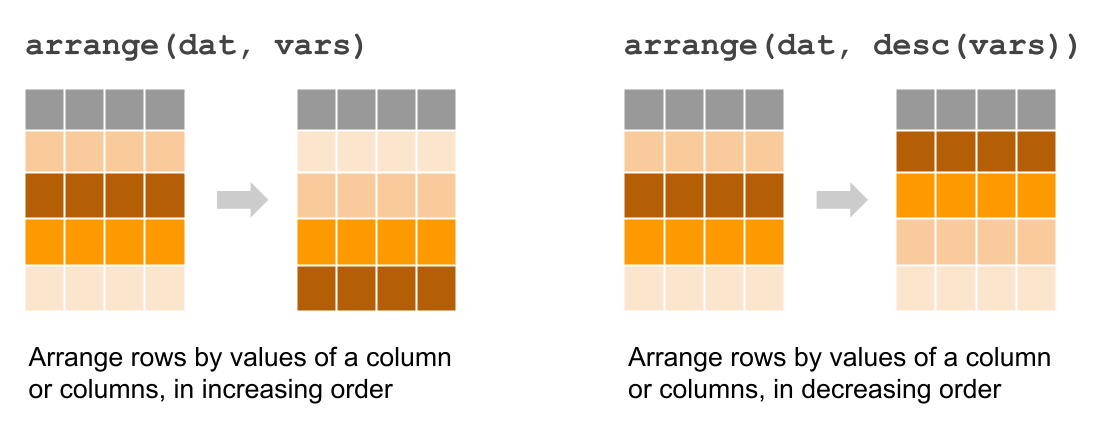
\includegraphics[width=0.85\linewidth]{images/dplyr-arrange} 

}

\caption{Arranging rows}\label{fig:unnamed-chunk-26}
\end{figure}

Say you want to arrange the contents of the average summary table, by taking
into account the column \texttt{avg\_wind}:

\begin{Shaded}
\begin{Highlighting}[]
\FunctionTok{arrange}\NormalTok{(avg\_wind\_pressure\_75, avg\_wind)}
\end{Highlighting}
\end{Shaded}

\begin{verbatim}
## # A tibble: 3 x 3
##   name     avg_wind avg_pressure
##   <chr>       <dbl>        <dbl>
## 1 Caroline     38.9        1002.
## 2 Amy          46.5         995.
## 3 Doris        73.7         983.
\end{verbatim}

Likewise, you can also arrange the averages by \texttt{avg\_pressure}:

\begin{Shaded}
\begin{Highlighting}[]
\FunctionTok{arrange}\NormalTok{(avg\_wind\_pressure\_75, avg\_pressure)}
\end{Highlighting}
\end{Shaded}

\begin{verbatim}
## # A tibble: 3 x 3
##   name     avg_wind avg_pressure
##   <chr>       <dbl>        <dbl>
## 1 Doris        73.7         983.
## 2 Amy          46.5         995.
## 3 Caroline     38.9        1002.
\end{verbatim}

The default behavior of \texttt{arrange()} is to organize rows in increasing order.
But what if you want to organize rows in decreasing order? No problem, just
use the auxiliary function \texttt{desc()} to indicate that rows should be arranged
decreasingly:

\begin{Shaded}
\begin{Highlighting}[]
\FunctionTok{arrange}\NormalTok{(avg\_wind\_pressure\_75, }\FunctionTok{desc}\NormalTok{(avg\_wind))}
\end{Highlighting}
\end{Shaded}

\begin{verbatim}
## # A tibble: 3 x 3
##   name     avg_wind avg_pressure
##   <chr>       <dbl>        <dbl>
## 1 Doris        73.7         983.
## 2 Amy          46.5         995.
## 3 Caroline     38.9        1002.
\end{verbatim}

\hypertarget{further-inspection-of-1975-storm-amy}{%
\section{Further inspection of 1975 storm Amy}\label{further-inspection-of-1975-storm-amy}}

Let's focus on a specific storm, for example storm \texttt{Amy} in 1975. For sake of
simplicity, we are going to create a table \texttt{amy75} containing the values of
this storm:

\begin{Shaded}
\begin{Highlighting}[]
\NormalTok{amy75 }\OtherTok{\textless{}{-}} \FunctionTok{filter}\NormalTok{(storms75, name }\SpecialCharTok{==} \StringTok{"Amy"}\NormalTok{)}
\NormalTok{amy75}
\end{Highlighting}
\end{Shaded}

\begin{verbatim}
## # A tibble: 30 x 13
##    name   year month   day  hour   lat  long status        categ~1  wind press~2
##    <chr> <dbl> <dbl> <int> <dbl> <dbl> <dbl> <chr>         <ord>   <int>   <int>
##  1 Amy    1975     6    27     0  27.5 -79   tropical dep~ -1         25    1013
##  2 Amy    1975     6    27     6  28.5 -79   tropical dep~ -1         25    1013
##  3 Amy    1975     6    27    12  29.5 -79   tropical dep~ -1         25    1013
##  4 Amy    1975     6    27    18  30.5 -79   tropical dep~ -1         25    1013
##  5 Amy    1975     6    28     0  31.5 -78.8 tropical dep~ -1         25    1012
##  6 Amy    1975     6    28     6  32.4 -78.7 tropical dep~ -1         25    1012
##  7 Amy    1975     6    28    12  33.3 -78   tropical dep~ -1         25    1011
##  8 Amy    1975     6    28    18  34   -77   tropical dep~ -1         30    1006
##  9 Amy    1975     6    29     0  34.4 -75.8 tropical sto~ 0          35    1004
## 10 Amy    1975     6    29     6  34   -74.8 tropical sto~ 0          40    1002
## # ... with 20 more rows, 2 more variables: tropicalstorm_force_diameter <int>,
## #   hurricane_force_diameter <int>, and abbreviated variable names 1: category,
## #   2: pressure
\end{verbatim}

Here's a couple of questions that we could investigate:

\begin{itemize}
\item
  which are the \texttt{status} categories for Amy?
\item
  during which months was Amy active? and for how many days?
\item
  what are the basic summary statistics for \texttt{wind} and \texttt{pressure}?
\end{itemize}

\begin{Shaded}
\begin{Highlighting}[]
\CommentTok{\# which are the \textasciigrave{}status\textasciigrave{} categories for Amy?}
\FunctionTok{distinct}\NormalTok{(amy75, status)}
\end{Highlighting}
\end{Shaded}

\begin{verbatim}
## # A tibble: 2 x 1
##   status             
##   <chr>              
## 1 tropical depression
## 2 tropical storm
\end{verbatim}

\begin{Shaded}
\begin{Highlighting}[]
\CommentTok{\# during which months was Amy active?}
\FunctionTok{distinct}\NormalTok{(amy75, month)}
\end{Highlighting}
\end{Shaded}

\begin{verbatim}
## # A tibble: 2 x 1
##   month
##   <dbl>
## 1     6
## 2     7
\end{verbatim}

\begin{Shaded}
\begin{Highlighting}[]
\CommentTok{\# for how many days was Amy active?}
\FunctionTok{count}\NormalTok{(}\FunctionTok{distinct}\NormalTok{(amy75, day))}
\end{Highlighting}
\end{Shaded}

\begin{verbatim}
## # A tibble: 1 x 1
##       n
##   <int>
## 1     8
\end{verbatim}

\begin{Shaded}
\begin{Highlighting}[]
\CommentTok{\# summary statistics for wind}
\FunctionTok{summary}\NormalTok{(}\FunctionTok{select}\NormalTok{(amy75, wind))}
\end{Highlighting}
\end{Shaded}

\begin{verbatim}
##       wind      
##  Min.   :25.00  
##  1st Qu.:31.25  
##  Median :50.00  
##  Mean   :46.50  
##  3rd Qu.:60.00  
##  Max.   :60.00
\end{verbatim}

\begin{Shaded}
\begin{Highlighting}[]
\CommentTok{\# summary statistics for pressure}
\FunctionTok{summary}\NormalTok{(}\FunctionTok{select}\NormalTok{(amy75, pressure))}
\end{Highlighting}
\end{Shaded}

\begin{verbatim}
##     pressure     
##  Min.   : 981.0  
##  1st Qu.: 986.0  
##  Median : 987.0  
##  Mean   : 995.1  
##  3rd Qu.:1005.5  
##  Max.   :1013.0
\end{verbatim}

\begin{center}\rule{0.5\linewidth}{0.5pt}\end{center}

\hypertarget{your-turn-2}{%
\subsection{Your Turn}\label{your-turn-2}}

\begin{itemize}
\item
  Use \texttt{"dplyr"} functions/commands to create a table (e.g.~tibble)
  \texttt{max\_wind\_pressure\_75} containing columns: 1)\texttt{name} of
  storm, 2) \texttt{max\_wind} maximum wind speed, and 3) \texttt{max\_pressure} maximum pressure
\item
  Use \texttt{"dplyr"} functions/commands to create a table (e.g.~tibble)
  \texttt{wind\_stats\_75} containing columns: 1)\texttt{name} of storm, 2) \texttt{min\_wind} minimum
  wind speed, 3) \texttt{avg\_wind} mean wind speed, 4) \texttt{med\_wind} median wind speed,
  and 5) \texttt{max\_wind} maximum wind speed.
\end{itemize}

\hypertarget{basic-maps}{%
\chapter{Basic Maps}\label{basic-maps}}

In the previous chapters, you were introduced to the basics of \texttt{"dplyr"} and
\texttt{"ggplot2"}, performing various operations on the data \texttt{storms}. Because this
data set contains geographical information such as longitude and latitude, we
need to take a further step in this module in order to learn about plotting
basic geographical maps.

You will need the following packages:

\begin{Shaded}
\begin{Highlighting}[]
\FunctionTok{library}\NormalTok{(tidyverse)      }\CommentTok{\# for syntactic manipulation of tables}
\FunctionTok{library}\NormalTok{(maps)           }\CommentTok{\# for drawing basic geographical maps}
\end{Highlighting}
\end{Shaded}

and the following objects:

\begin{Shaded}
\begin{Highlighting}[]
\NormalTok{storms75 }\OtherTok{\textless{}{-}} \FunctionTok{filter}\NormalTok{(storms, year }\SpecialCharTok{==} \DecValTok{1975}\NormalTok{)}
\end{Highlighting}
\end{Shaded}

\hypertarget{graphing-maps}{%
\section{Graphing Maps}\label{graphing-maps}}

In this part, we give a basic exposure to plotting maps with \texttt{"ggplot2"}
and \texttt{"maps"}. Keep in mind that there is a wide array of packages for graphing
all sorts of maps, and geospatial information. Good resources to look at are:

\begin{itemize}
\item
  \emph{Drawing beautiful maps programmatically with R, sf and ggplot2} by Mel Moreno and Mathieu Basille; \url{https://www.r-spatial.org/r/2018/10/25/ggplot2-sf.html}
\item
  \emph{Geocomputation with R} by Robin Lovelace, Jakub Nowosad, and Jannes Muenchow; \url{https://geocompr.robinlovelace.net}
\item
  \emph{Making Maps with R} by Eric C. Anderson; \url{https://eriqande.github.io/rep-res-web/lectures/making-maps-with-R.html}
\end{itemize}

\hypertarget{plotting-location-of-storm-records}{%
\subsection{Plotting location of storm records}\label{plotting-location-of-storm-records}}

For illustration purposes, we continue using the data frame \texttt{storms75}. Having
latitude and longitude, we can make a scatterplot to see the location of
the storm records. Recall that the \texttt{ggplot} function to do this is
\texttt{geom\_point()}. To distinguish each storm, we can color the
dots by taking into account the different storm names. This involves \emph{mapping}
the column \texttt{name} to the \texttt{color} attribute:

\begin{Shaded}
\begin{Highlighting}[]
\FunctionTok{ggplot}\NormalTok{(}\AttributeTok{data =}\NormalTok{ storms75, }\FunctionTok{aes}\NormalTok{(}\AttributeTok{x =}\NormalTok{ long, }\AttributeTok{y =}\NormalTok{ lat, }\AttributeTok{color =}\NormalTok{ name)) }\SpecialCharTok{+} 
  \FunctionTok{geom\_point}\NormalTok{()}
\end{Highlighting}
\end{Shaded}

\begin{center}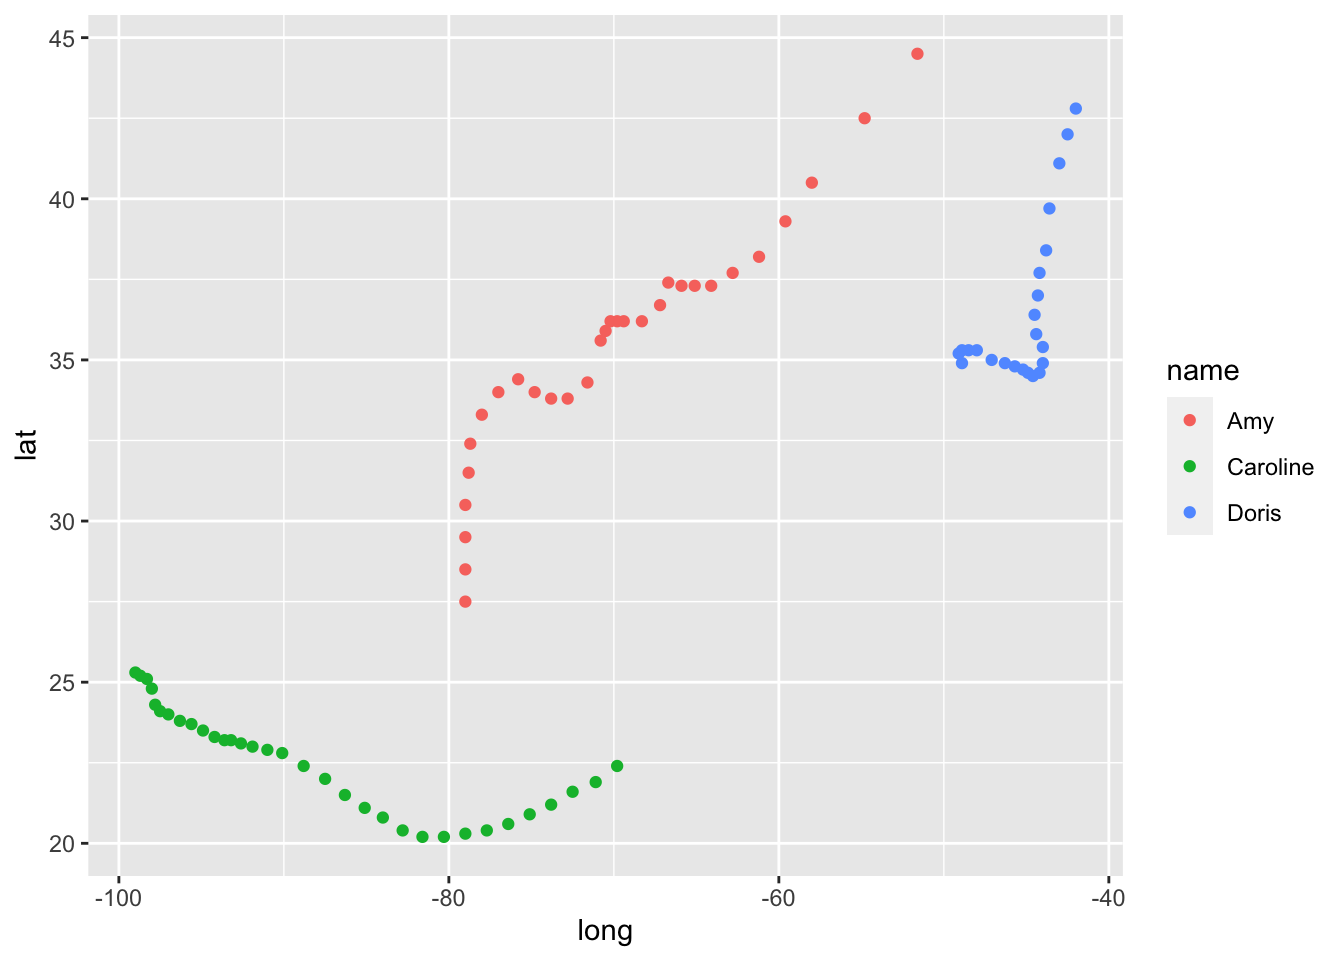
\includegraphics[width=0.8\linewidth]{R-tidy-hurricanes_files/figure-latex/plot-map0-storms75-1} \end{center}

Keep in mind that the previous command can also be written as:

\begin{Shaded}
\begin{Highlighting}[]
\CommentTok{\# alternative ways to write equivalent commands}
\FunctionTok{ggplot}\NormalTok{(}\AttributeTok{data =}\NormalTok{ storms75) }\SpecialCharTok{+}  
  \FunctionTok{geom\_point}\NormalTok{(}\FunctionTok{aes}\NormalTok{(}\AttributeTok{x =}\NormalTok{ long, }\AttributeTok{y =}\NormalTok{ lat, }\AttributeTok{color =}\NormalTok{ name))}

\FunctionTok{ggplot}\NormalTok{() }\SpecialCharTok{+}  
  \FunctionTok{geom\_point}\NormalTok{(}\AttributeTok{data =}\NormalTok{ storms75, }\FunctionTok{aes}\NormalTok{(}\AttributeTok{x =}\NormalTok{ long, }\AttributeTok{y =}\NormalTok{ lat, }\AttributeTok{color =}\NormalTok{ name))}
\end{Highlighting}
\end{Shaded}

The above scatterplot is a good starting point to visualize the location of the
storm records, but it would be nice to have an actual image of a map. Let's
see how to do this in the following subsections.

\hypertarget{basic-map}{%
\subsection{Basic map}\label{basic-map}}

One of the oldest ways to plot maps in R is with the package \texttt{"maps"}. Nowadays,
there are better packages for geospatial data and making maps, but let's not
worry about them at this moment.

One rudimentary way to plot a map is by first getting data of the world.
\texttt{"ggplot2"} provides the function \texttt{map\_data()} to create the required data
table with geospatial information of a world map. All you have to do is specify
the name of the map provided by the \texttt{"maps"} package. In this example, let's
use the \texttt{"world"} map. Once we have this data, we can use it with \texttt{ggplot()}
and a \texttt{geom\_polygon()} layer like this:

\begin{Shaded}
\begin{Highlighting}[]
\CommentTok{\# world map data}
\NormalTok{world\_map }\OtherTok{\textless{}{-}} \FunctionTok{map\_data}\NormalTok{(}\StringTok{"world"}\NormalTok{)}

\CommentTok{\# a default world map}
\FunctionTok{ggplot}\NormalTok{() }\SpecialCharTok{+} 
  \FunctionTok{geom\_polygon}\NormalTok{(}\AttributeTok{data =}\NormalTok{ world\_map, }
               \FunctionTok{aes}\NormalTok{(}\AttributeTok{x =}\NormalTok{ long, }\AttributeTok{y =}\NormalTok{ lat, }\AttributeTok{group =}\NormalTok{ group))}
\end{Highlighting}
\end{Shaded}

\begin{center}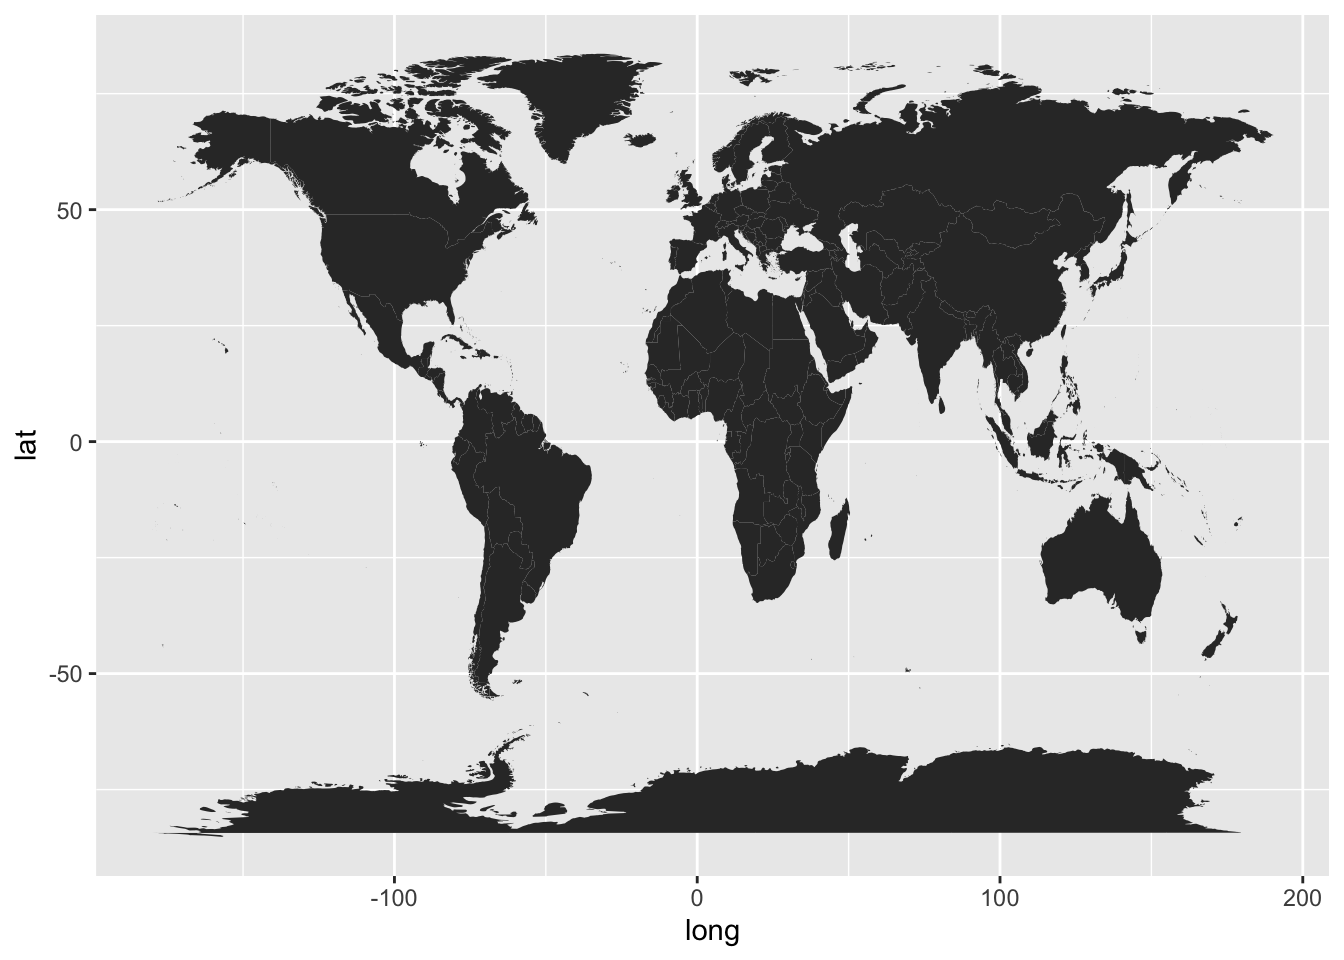
\includegraphics[width=0.8\linewidth]{R-tidy-hurricanes_files/figure-latex/plot-map1-storms75-1} \end{center}

In the above command, notice how we specify the \texttt{data} argument inside
\texttt{geom\_polygon()} instead of inside \texttt{ggplot()}. We do this because the data
frame \texttt{world\_map} is used to graph the layer of the map. We still need to add
another layer---via \texttt{geom\_point()}---for the coordinates indicating the
position of each storm's record.

To handle the code more easily, let's modify the map, and create a \texttt{"ggplot"}
object called \texttt{gg\_world}. We'll use this object as our ``canvas'' for plotting
the storm locations:

\begin{Shaded}
\begin{Highlighting}[]
\CommentTok{\# map "canvas" stored as gg\_world}
\NormalTok{gg\_world }\OtherTok{\textless{}{-}} \FunctionTok{ggplot}\NormalTok{() }\SpecialCharTok{+} 
  \FunctionTok{geom\_polygon}\NormalTok{(}\AttributeTok{data =}\NormalTok{ world\_map, }
               \FunctionTok{aes}\NormalTok{(}\AttributeTok{x =}\NormalTok{ long, }\AttributeTok{y =}\NormalTok{ lat, }\AttributeTok{group =}\NormalTok{ group), }
               \AttributeTok{fill =} \StringTok{"gray95"}\NormalTok{, }\AttributeTok{colour =} \StringTok{"gray70"}\NormalTok{, }\AttributeTok{size =} \FloatTok{0.2}\NormalTok{) }\SpecialCharTok{+}
  \FunctionTok{theme\_bw}\NormalTok{()}

\NormalTok{gg\_world}
\end{Highlighting}
\end{Shaded}

\begin{center}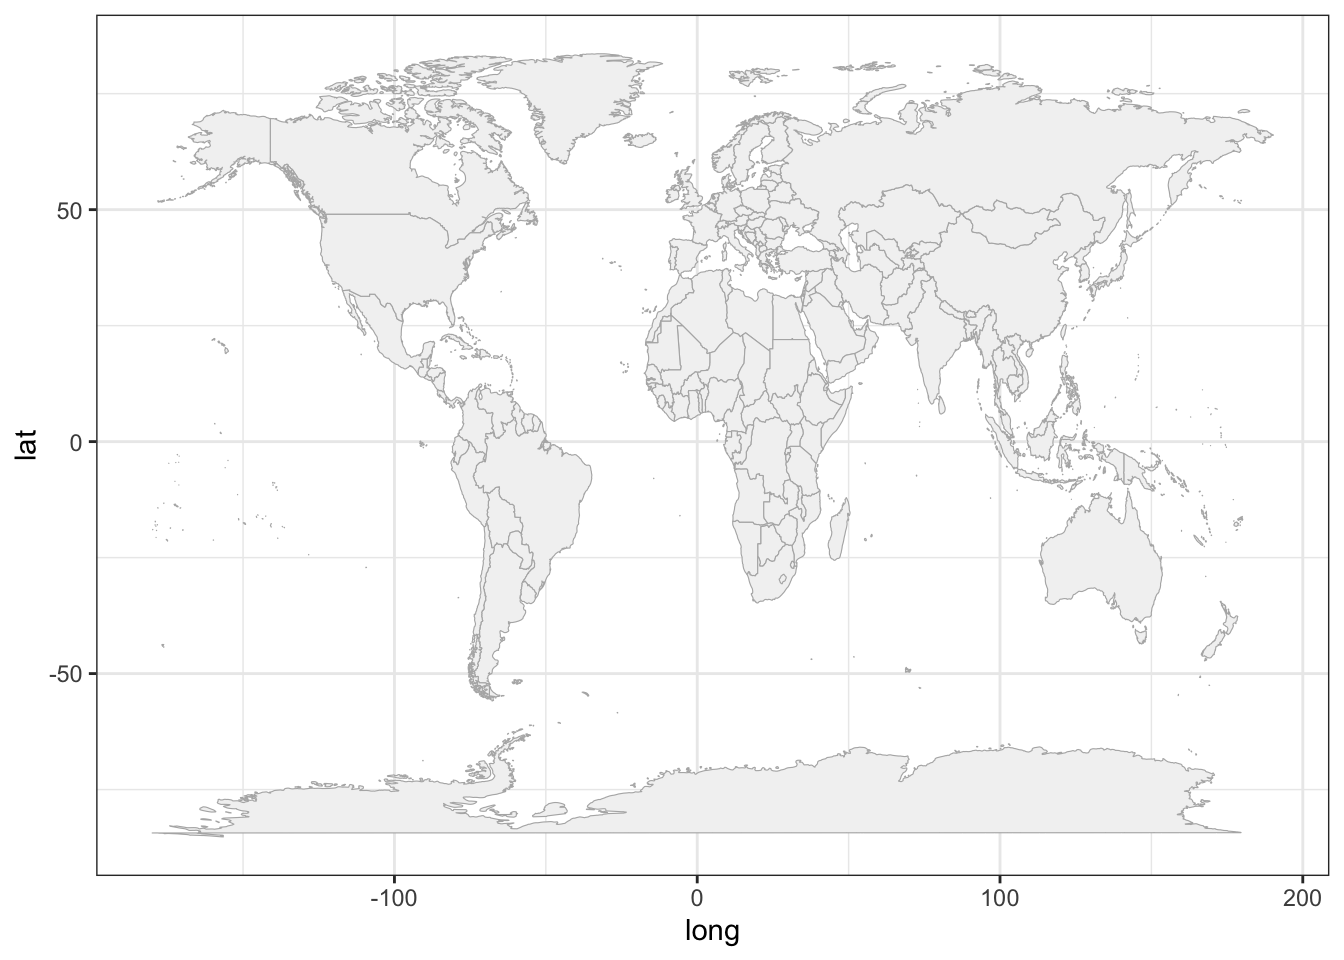
\includegraphics[width=0.8\linewidth]{R-tidy-hurricanes_files/figure-latex/plot-map2-storms75-1} \end{center}

\hypertarget{mapping-1975-storms}{%
\subsection{Mapping 1975 Storms}\label{mapping-1975-storms}}

Now that we know how to plot a map with \texttt{ggplot()}, we can add the points of
the storm records. This is done with \texttt{geom\_point()}, and specifying \texttt{storms75}
as the \texttt{data} argument inside this function. In other words, we are using two
separate data frames. One is \texttt{world\_map}, used to draw the polygons of the map;
the other one is \texttt{stomrs75} to graph the dots of each storm. Notice also that
there are no inputs provided to the function \texttt{ggplot()}.

\begin{Shaded}
\begin{Highlighting}[]
\CommentTok{\# world map, adding storms in 1975}
\NormalTok{gg\_world }\SpecialCharTok{+}
  \FunctionTok{geom\_point}\NormalTok{(}\AttributeTok{data =}\NormalTok{ storms75,}
             \FunctionTok{aes}\NormalTok{(}\AttributeTok{x =}\NormalTok{ long, }\AttributeTok{y =}\NormalTok{ lat, }\AttributeTok{color =}\NormalTok{ name))}
\end{Highlighting}
\end{Shaded}

\begin{center}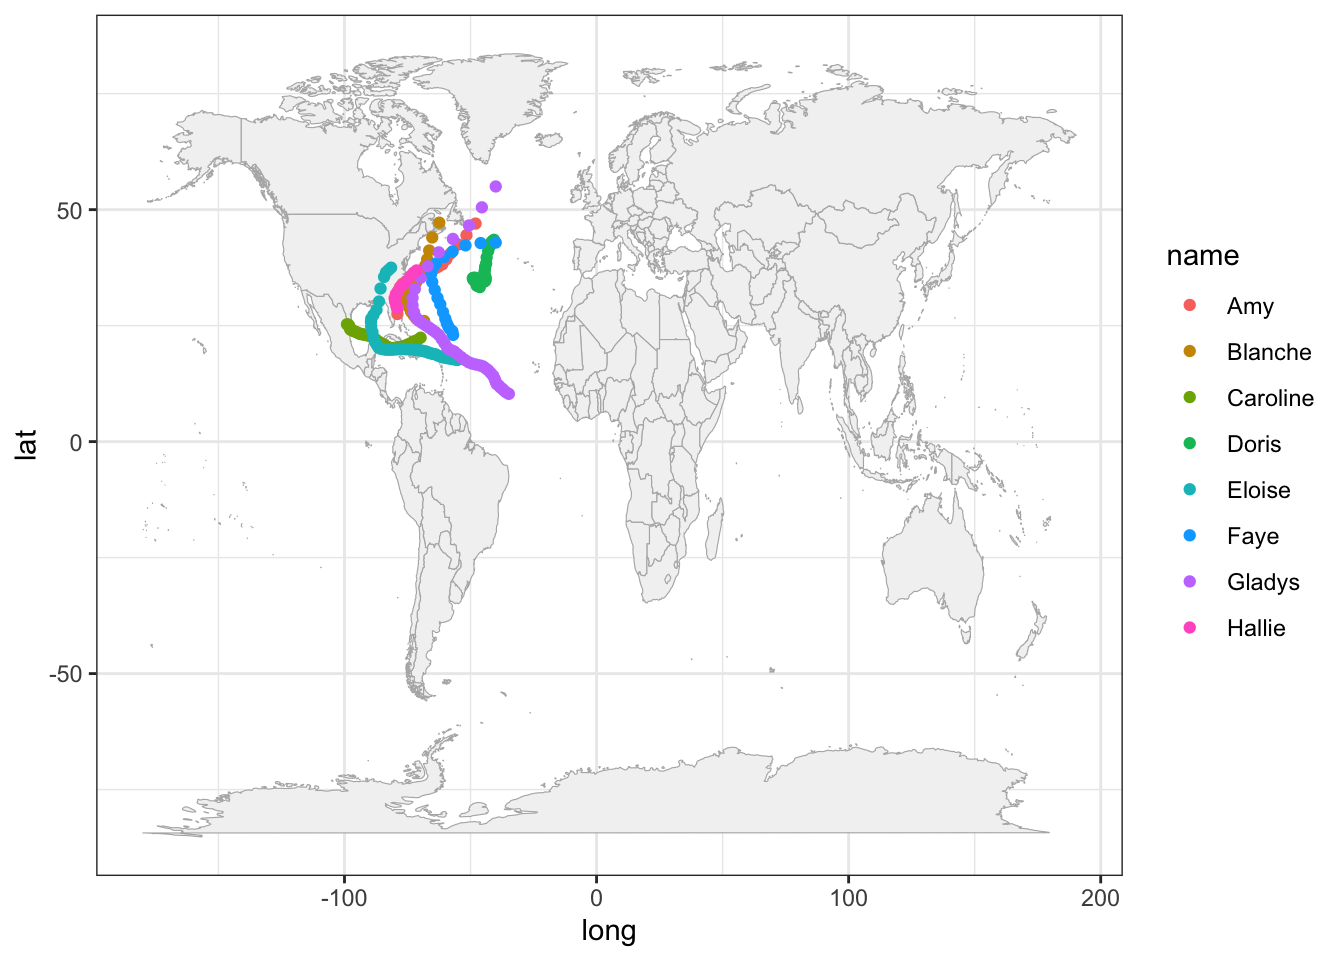
\includegraphics[width=0.8\linewidth]{R-tidy-hurricanes_files/figure-latex/plot-map3-storms75-1} \end{center}

Because the analyzed hurricanes occurred in the North Atlantic basin, we can
focus on that region by modifying the x-and-y axis limits:

\begin{Shaded}
\begin{Highlighting}[]
\CommentTok{\# zoom{-}in}
\NormalTok{gg\_world }\SpecialCharTok{+}
  \FunctionTok{geom\_point}\NormalTok{(}\AttributeTok{data =}\NormalTok{ storms75,}
             \FunctionTok{aes}\NormalTok{(}\AttributeTok{x =}\NormalTok{ long, }\AttributeTok{y =}\NormalTok{ lat, }\AttributeTok{color =}\NormalTok{ name)) }\SpecialCharTok{+}
  \FunctionTok{xlim}\NormalTok{(}\FunctionTok{c}\NormalTok{(}\SpecialCharTok{{-}}\DecValTok{150}\NormalTok{, }\DecValTok{0}\NormalTok{)) }\SpecialCharTok{+} 
  \FunctionTok{ylim}\NormalTok{(}\FunctionTok{c}\NormalTok{(}\DecValTok{0}\NormalTok{, }\DecValTok{90}\NormalTok{))}
\end{Highlighting}
\end{Shaded}

\begin{center}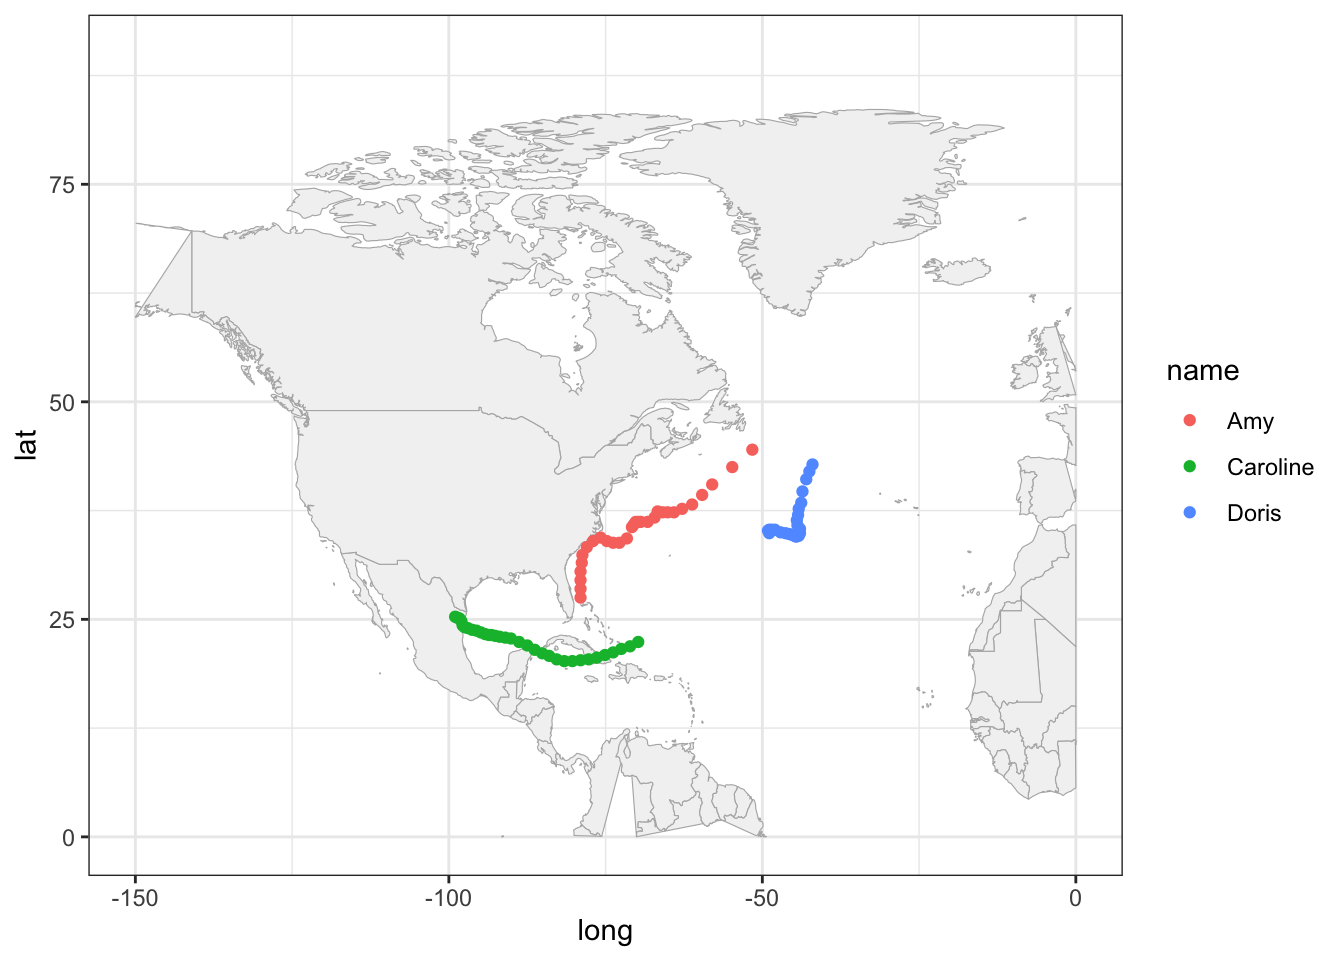
\includegraphics[width=0.8\linewidth]{R-tidy-hurricanes_files/figure-latex/plot-map4-storms75-1} \end{center}

It's worth mentioning that this zooming-in has a secondary effect of distorting
some of the polygons. For example, Alaska seems to get cut in half. Also the
polygon of Colombia is incomplete. Ignoring these distortions for now, we can
continue exploring things by taking into account more variables. For instance,
let's map the \texttt{wind} speed to the \texttt{size} argument of points.

\begin{Shaded}
\begin{Highlighting}[]
\NormalTok{gg\_world }\SpecialCharTok{+}
  \FunctionTok{geom\_point}\NormalTok{(}\AttributeTok{data =}\NormalTok{ storms75,}
             \FunctionTok{aes}\NormalTok{(}\AttributeTok{x =}\NormalTok{ long, }\AttributeTok{y =}\NormalTok{ lat, }\AttributeTok{color =}\NormalTok{ name, }\AttributeTok{size =}\NormalTok{ wind),}
             \AttributeTok{alpha =} \FloatTok{0.5}\NormalTok{) }\SpecialCharTok{+}
  \FunctionTok{xlim}\NormalTok{(}\FunctionTok{c}\NormalTok{(}\SpecialCharTok{{-}}\DecValTok{150}\NormalTok{, }\DecValTok{0}\NormalTok{)) }\SpecialCharTok{+} 
  \FunctionTok{ylim}\NormalTok{(}\FunctionTok{c}\NormalTok{(}\DecValTok{0}\NormalTok{, }\DecValTok{90}\NormalTok{))}
\end{Highlighting}
\end{Shaded}

\begin{center}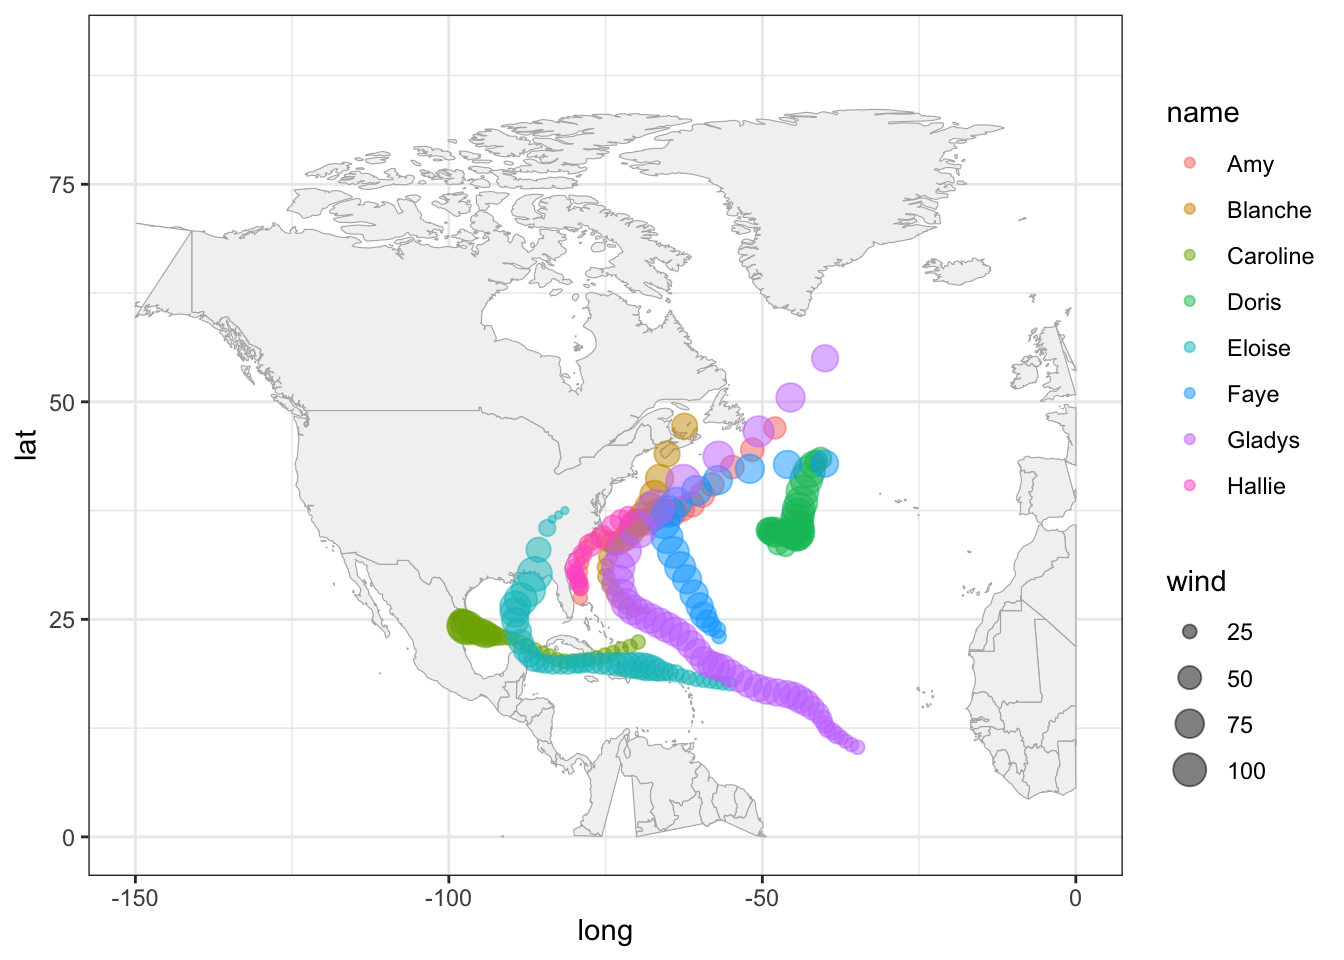
\includegraphics[width=0.8\linewidth]{R-tidy-hurricanes_files/figure-latex/plot-map5-storms75-1} \end{center}

A very similar appearance can be achieved by replacing \texttt{geom\_point()} with
\texttt{geom\_path()}:

\begin{Shaded}
\begin{Highlighting}[]
\NormalTok{gg\_world }\SpecialCharTok{+}
  \FunctionTok{geom\_path}\NormalTok{(}\AttributeTok{data =}\NormalTok{ storms75,}
             \FunctionTok{aes}\NormalTok{(}\AttributeTok{x =}\NormalTok{ long, }\AttributeTok{y =}\NormalTok{ lat, }\AttributeTok{color =}\NormalTok{ name, }\AttributeTok{size =}\NormalTok{ wind),}
             \AttributeTok{lineend =} \StringTok{"round"}\NormalTok{, }\AttributeTok{alpha =} \FloatTok{0.4}\NormalTok{) }\SpecialCharTok{+}
  \FunctionTok{xlim}\NormalTok{(}\FunctionTok{c}\NormalTok{(}\SpecialCharTok{{-}}\DecValTok{150}\NormalTok{, }\DecValTok{0}\NormalTok{)) }\SpecialCharTok{+} 
  \FunctionTok{ylim}\NormalTok{(}\FunctionTok{c}\NormalTok{(}\DecValTok{0}\NormalTok{, }\DecValTok{90}\NormalTok{))}
\end{Highlighting}
\end{Shaded}

\begin{center}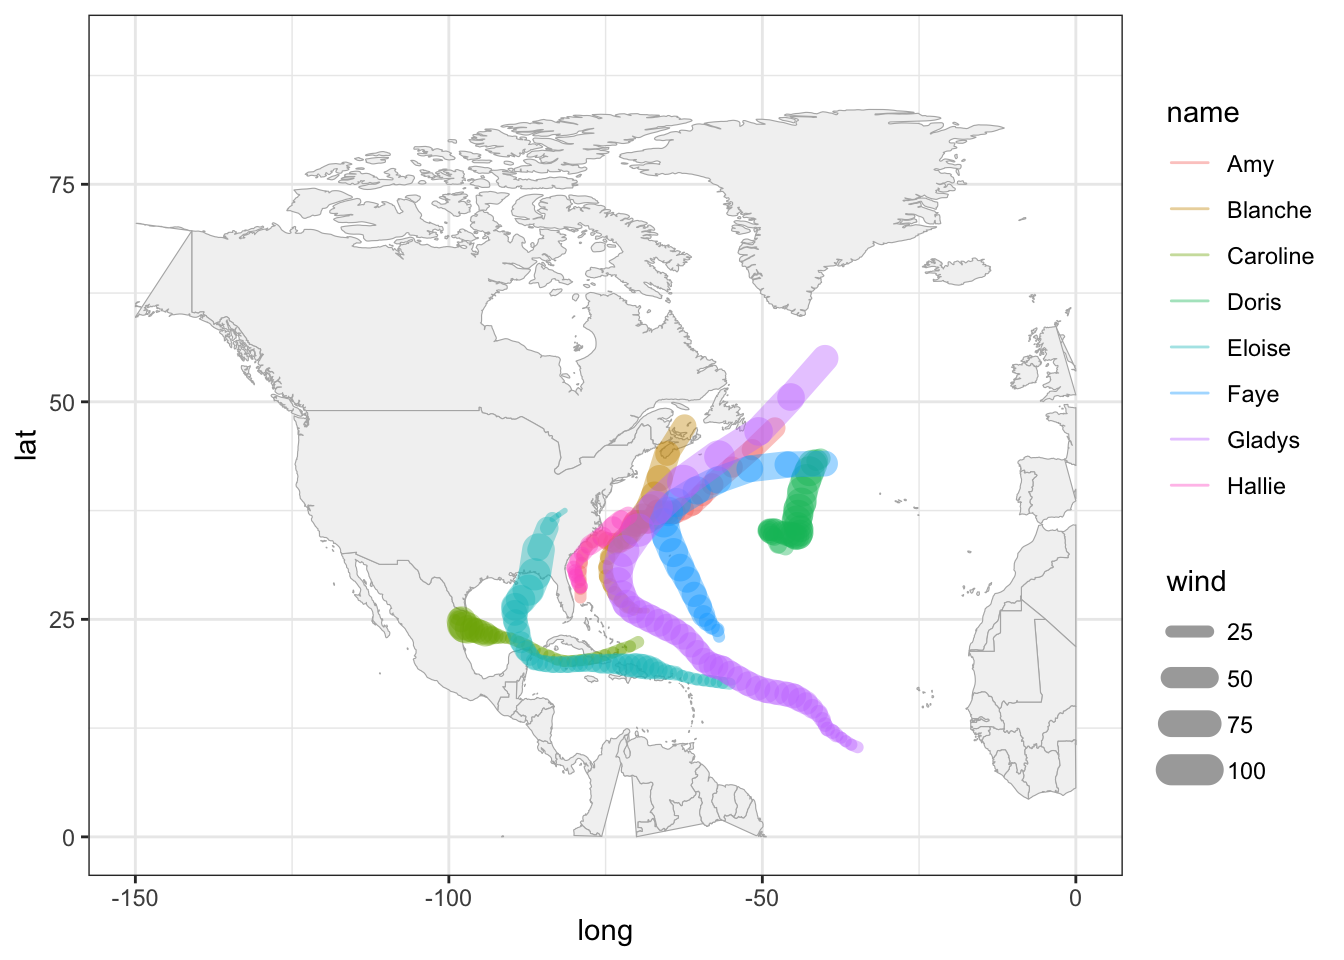
\includegraphics[width=0.8\linewidth]{R-tidy-hurricanes_files/figure-latex/plot-map6-storms75-1} \end{center}

\hypertarget{less-basic-maps}{%
\chapter{Less Basic Maps}\label{less-basic-maps}}

The code in this chapter requires the following packages:

\begin{Shaded}
\begin{Highlighting}[]
\FunctionTok{library}\NormalTok{(tidyverse)          }\CommentTok{\# for syntactic manipulation of tables}
\FunctionTok{library}\NormalTok{(rnaturalearth)      }\CommentTok{\# world map data from Natural Earth}
\FunctionTok{library}\NormalTok{(rnaturalearthdata)  }\CommentTok{\# companion package of rnaturalearth}
\end{Highlighting}
\end{Shaded}

and the following table for storms in 1975:

\begin{Shaded}
\begin{Highlighting}[]
\NormalTok{storms75 }\OtherTok{\textless{}{-}} \FunctionTok{filter}\NormalTok{(storms, year }\SpecialCharTok{==} \DecValTok{1975}\NormalTok{)}
\end{Highlighting}
\end{Shaded}

\hypertarget{more-mapping-approaches}{%
\section{More mapping approaches}\label{more-mapping-approaches}}

Another interesting map graphing approach is by using map-objects from the
package \texttt{"rnaturalearth"}.

We use the \texttt{ne\_countries()} function---from \texttt{"rnaturalearth"}---to get world
country polygons. In the following command, we specify a \texttt{medium} scale
resolution, and a returned object of class \texttt{"sf"} (simple features).

\begin{Shaded}
\begin{Highlighting}[]
\CommentTok{\# another world data frame}
\NormalTok{world\_df }\OtherTok{\textless{}{-}} \FunctionTok{ne\_countries}\NormalTok{(}\AttributeTok{scale =} \StringTok{"medium"}\NormalTok{, }\AttributeTok{returnclass =} \StringTok{"sf"}\NormalTok{)}
\FunctionTok{class}\NormalTok{(world\_df)}
\end{Highlighting}
\end{Shaded}

\begin{verbatim}
## [1] "sf"         "data.frame"
\end{verbatim}

Now we can pass \texttt{world\_df} to \texttt{ggplot()}, and use \texttt{geom\_sf()} which is the
function that allows us to visualize \emph{simple features} objects \texttt{"sf"}.

\begin{Shaded}
\begin{Highlighting}[]
\CommentTok{\# another world map (from "rnaturalearth")}
\FunctionTok{ggplot}\NormalTok{(}\AttributeTok{data =}\NormalTok{ world\_df) }\SpecialCharTok{+}
  \FunctionTok{geom\_sf}\NormalTok{() }\SpecialCharTok{+} 
  \FunctionTok{theme\_bw}\NormalTok{()}
\end{Highlighting}
\end{Shaded}

\begin{center}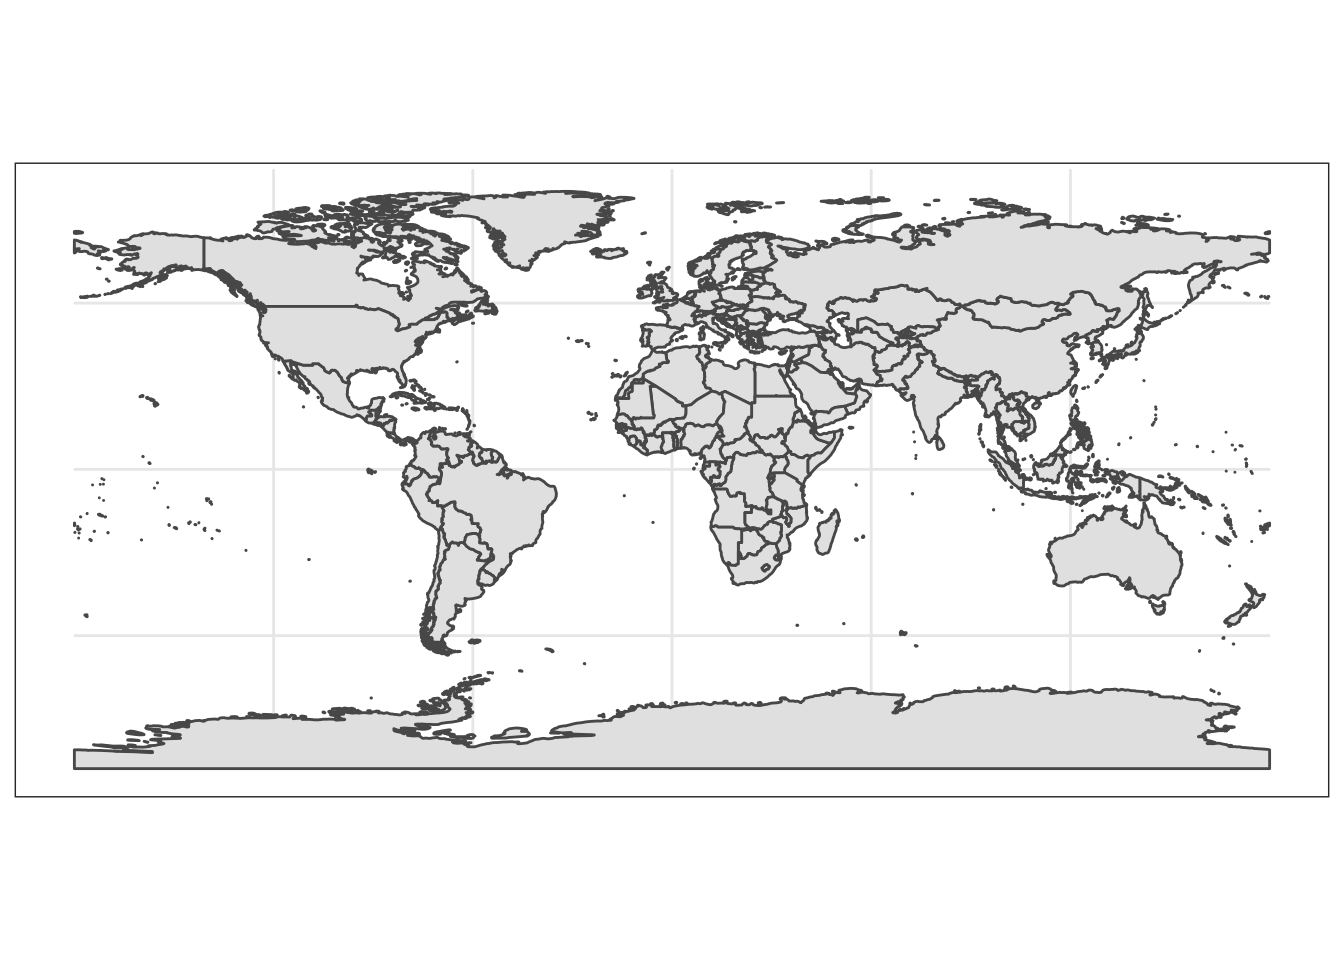
\includegraphics[width=0.8\linewidth]{R-tidy-hurricanes_files/figure-latex/world1-1} \end{center}

One advantage of using this other mapping approach is that we can zoom-in
without having distorted polygons. To focus on a specific region, we set the
x-axis and y-axis limits with the \texttt{coord\_sf()} function. Again, for coding
convenience, let's create another \texttt{"ggplot"} object

\begin{Shaded}
\begin{Highlighting}[]
\CommentTok{\# ggplot object to be used as a canvas}
\NormalTok{gg\_world2 }\OtherTok{\textless{}{-}} \FunctionTok{ggplot}\NormalTok{(}\AttributeTok{data =}\NormalTok{ world\_df) }\SpecialCharTok{+}
  \FunctionTok{geom\_sf}\NormalTok{() }\SpecialCharTok{+} 
  \FunctionTok{coord\_sf}\NormalTok{(}\AttributeTok{xlim =} \FunctionTok{c}\NormalTok{(}\SpecialCharTok{{-}}\DecValTok{150}\NormalTok{, }\DecValTok{0}\NormalTok{), }\AttributeTok{ylim =} \FunctionTok{c}\NormalTok{(}\DecValTok{0}\NormalTok{, }\DecValTok{90}\NormalTok{), }\AttributeTok{expand =} \ConstantTok{TRUE}\NormalTok{) }\SpecialCharTok{+}
  \FunctionTok{theme\_bw}\NormalTok{()}

\NormalTok{gg\_world2}
\end{Highlighting}
\end{Shaded}

\begin{center}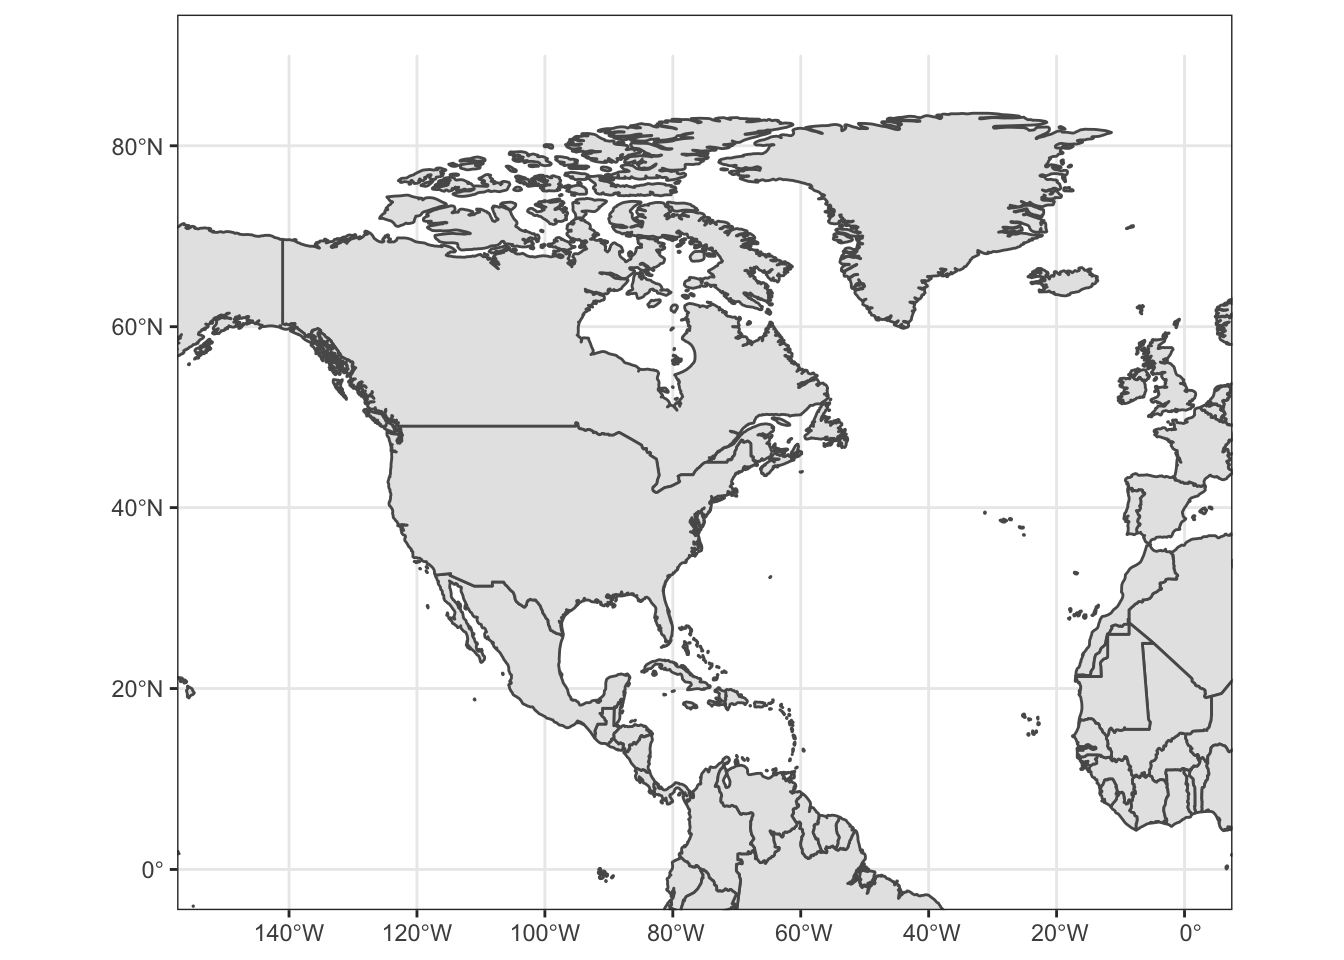
\includegraphics[width=0.8\linewidth]{R-tidy-hurricanes_files/figure-latex/world2-1} \end{center}

Now let's add the storms:

\begin{Shaded}
\begin{Highlighting}[]
\NormalTok{gg\_world2 }\SpecialCharTok{+} 
  \FunctionTok{geom\_path}\NormalTok{(}\AttributeTok{data =}\NormalTok{ storms75,}
            \FunctionTok{aes}\NormalTok{(}\AttributeTok{x =}\NormalTok{ long, }\AttributeTok{y =}\NormalTok{ lat, }\AttributeTok{color =}\NormalTok{ name),}
            \AttributeTok{lineend =} \StringTok{"round"}\NormalTok{, }\AttributeTok{size =} \DecValTok{2}\NormalTok{, }\AttributeTok{alpha =} \FloatTok{0.8}\NormalTok{)}
\end{Highlighting}
\end{Shaded}

\begin{center}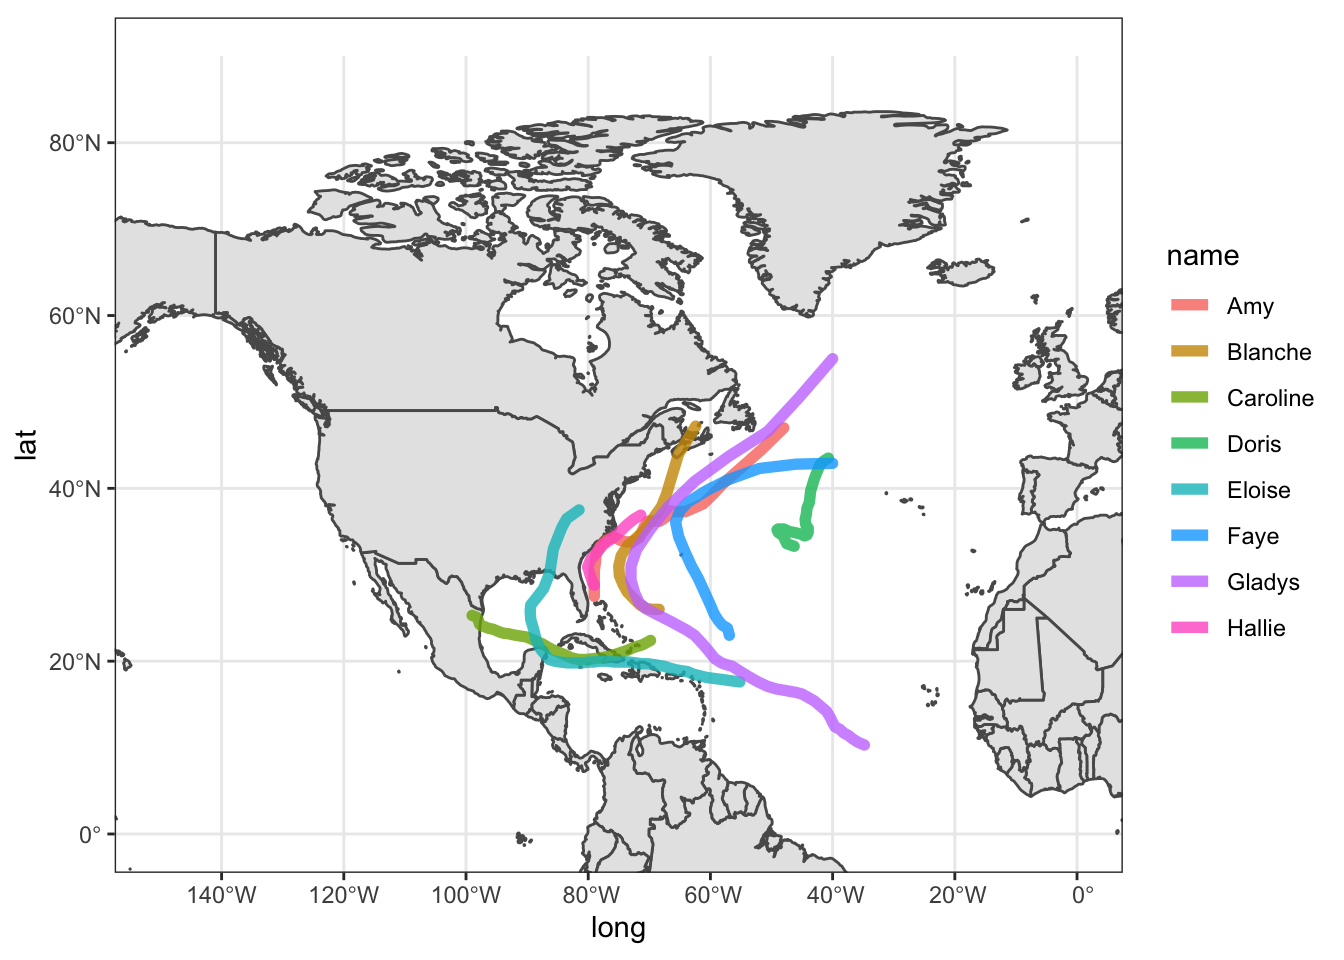
\includegraphics[width=0.8\linewidth]{R-tidy-hurricanes_files/figure-latex/storms75map5-1} \end{center}

\hypertarget{storms-from-1975-to-1980}{%
\subsection{Storms from 1975 to 1980}\label{storms-from-1975-to-1980}}

As a simple experiment, let's graph storms between 1975 and 1980 (six years).
First we create a dedicated data table \texttt{storms\_75\_80} to select the rows we are
interested in:

\begin{Shaded}
\begin{Highlighting}[]
\NormalTok{storms\_75\_80 }\OtherTok{\textless{}{-}} \FunctionTok{filter}\NormalTok{(storms, year }\SpecialCharTok{\%in\%} \DecValTok{1975}\SpecialCharTok{:}\DecValTok{1980}\NormalTok{)}
\end{Highlighting}
\end{Shaded}

And then we can use \texttt{facet\_wrap(\textasciitilde{}\ year)} to graph storms by year:

\begin{Shaded}
\begin{Highlighting}[]
\NormalTok{gg\_world2 }\SpecialCharTok{+}
  \FunctionTok{geom\_path}\NormalTok{(}\AttributeTok{data =}\NormalTok{ storms\_75\_80,}
             \FunctionTok{aes}\NormalTok{(}\AttributeTok{x =}\NormalTok{ long, }\AttributeTok{y =}\NormalTok{ lat, }\AttributeTok{group =}\NormalTok{ name),}
             \AttributeTok{lineend =} \StringTok{"round"}\NormalTok{) }\SpecialCharTok{+}
  \FunctionTok{xlim}\NormalTok{(}\FunctionTok{c}\NormalTok{(}\SpecialCharTok{{-}}\DecValTok{150}\NormalTok{, }\DecValTok{0}\NormalTok{)) }\SpecialCharTok{+} 
  \FunctionTok{ylim}\NormalTok{(}\FunctionTok{c}\NormalTok{(}\DecValTok{0}\NormalTok{, }\DecValTok{90}\NormalTok{)) }\SpecialCharTok{+} 
  \FunctionTok{facet\_wrap}\NormalTok{(}\SpecialCharTok{\textasciitilde{}}\NormalTok{ year)}
\end{Highlighting}
\end{Shaded}

\begin{center}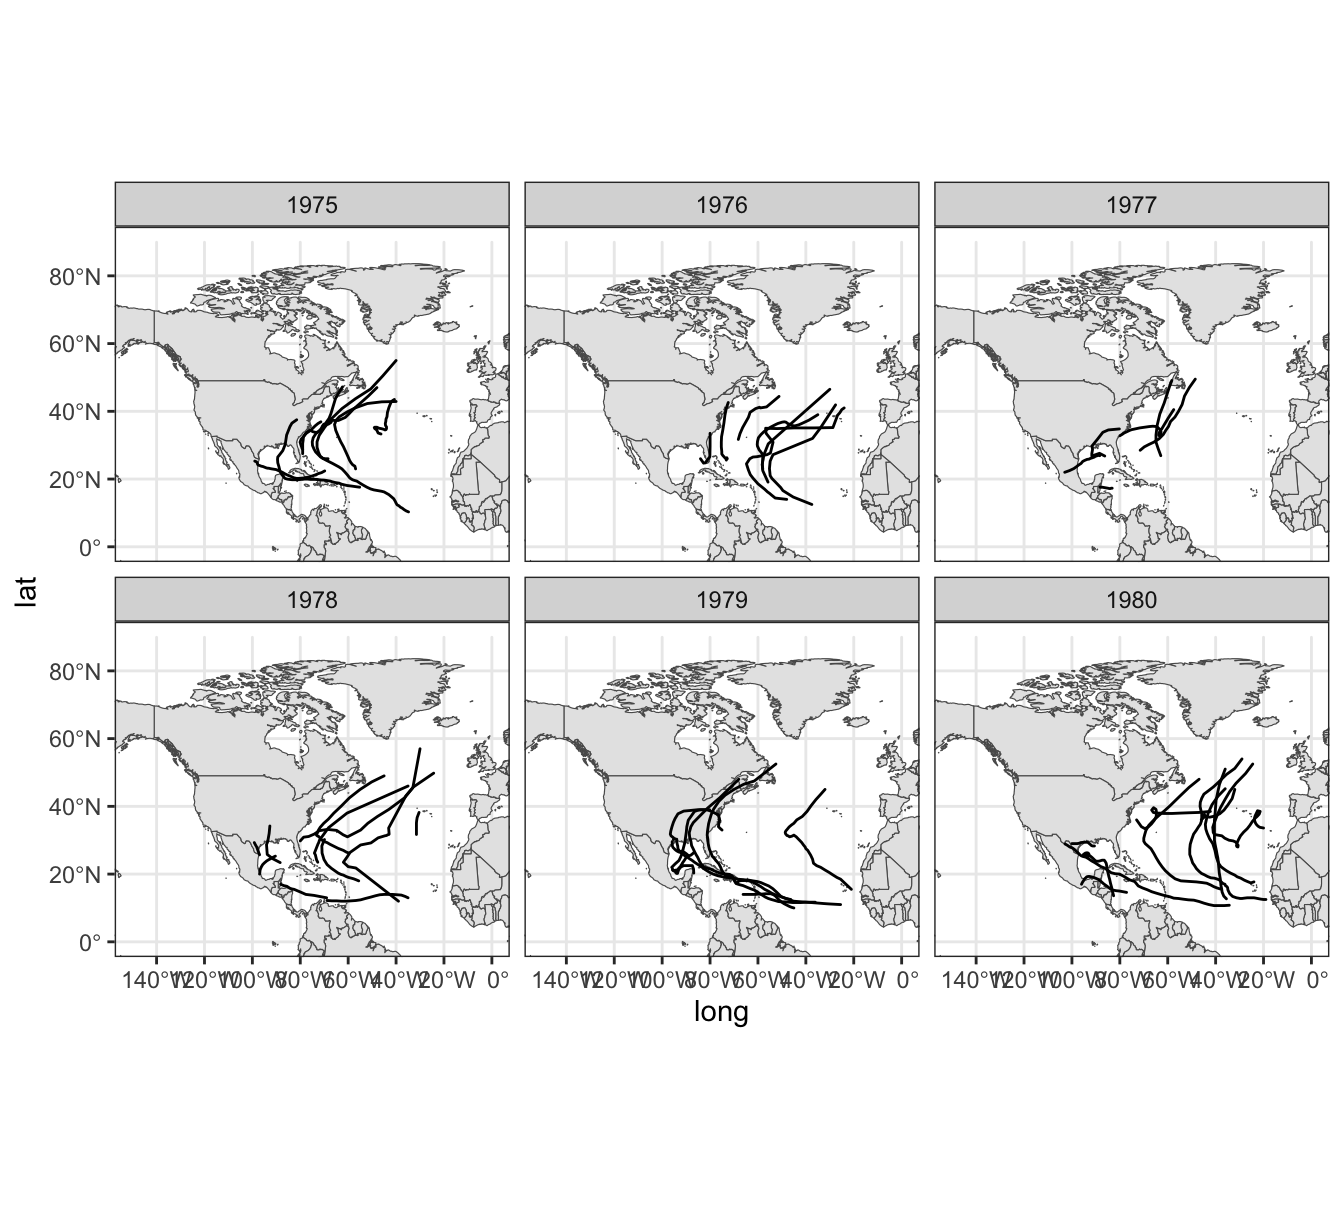
\includegraphics[width=0.9\linewidth]{R-tidy-hurricanes_files/figure-latex/world23-1} \end{center}

\hypertarget{part-1-summary}{%
\chapter{Part 1 Summary}\label{part-1-summary}}

So far, we've covered several functions from \texttt{"dplyr"}, as well as some other
functions in R:

\begin{itemize}
\tightlist
\item
  functions from \texttt{"dplyr"}

  \begin{itemize}
  \tightlist
  \item
    \texttt{pull()} and \texttt{select()}
  \item
    \texttt{filter()}
  \item
    \texttt{group\_by()}
  \item
    \texttt{arrange()} and \texttt{desc()}
  \item
    \texttt{count()}, \texttt{distinct()}, \texttt{summarise()}
  \end{itemize}
\item
  functions in base R

  \begin{itemize}
  \tightlist
  \item
    \texttt{unique()}, \texttt{sort()}, \texttt{mean()}, \texttt{summary()}
  \end{itemize}
\end{itemize}

\hypertarget{number-of-storms-per-year}{%
\section{Number of Storms per Year}\label{number-of-storms-per-year}}

If you recall, our first ggplot involved a barchart for the values in column
\texttt{year}

\begin{Shaded}
\begin{Highlighting}[]
\FunctionTok{ggplot}\NormalTok{(}\AttributeTok{data =}\NormalTok{ storms) }\SpecialCharTok{+} 
  \FunctionTok{geom\_bar}\NormalTok{(}\FunctionTok{aes}\NormalTok{(}\AttributeTok{x =}\NormalTok{ year))}
\end{Highlighting}
\end{Shaded}

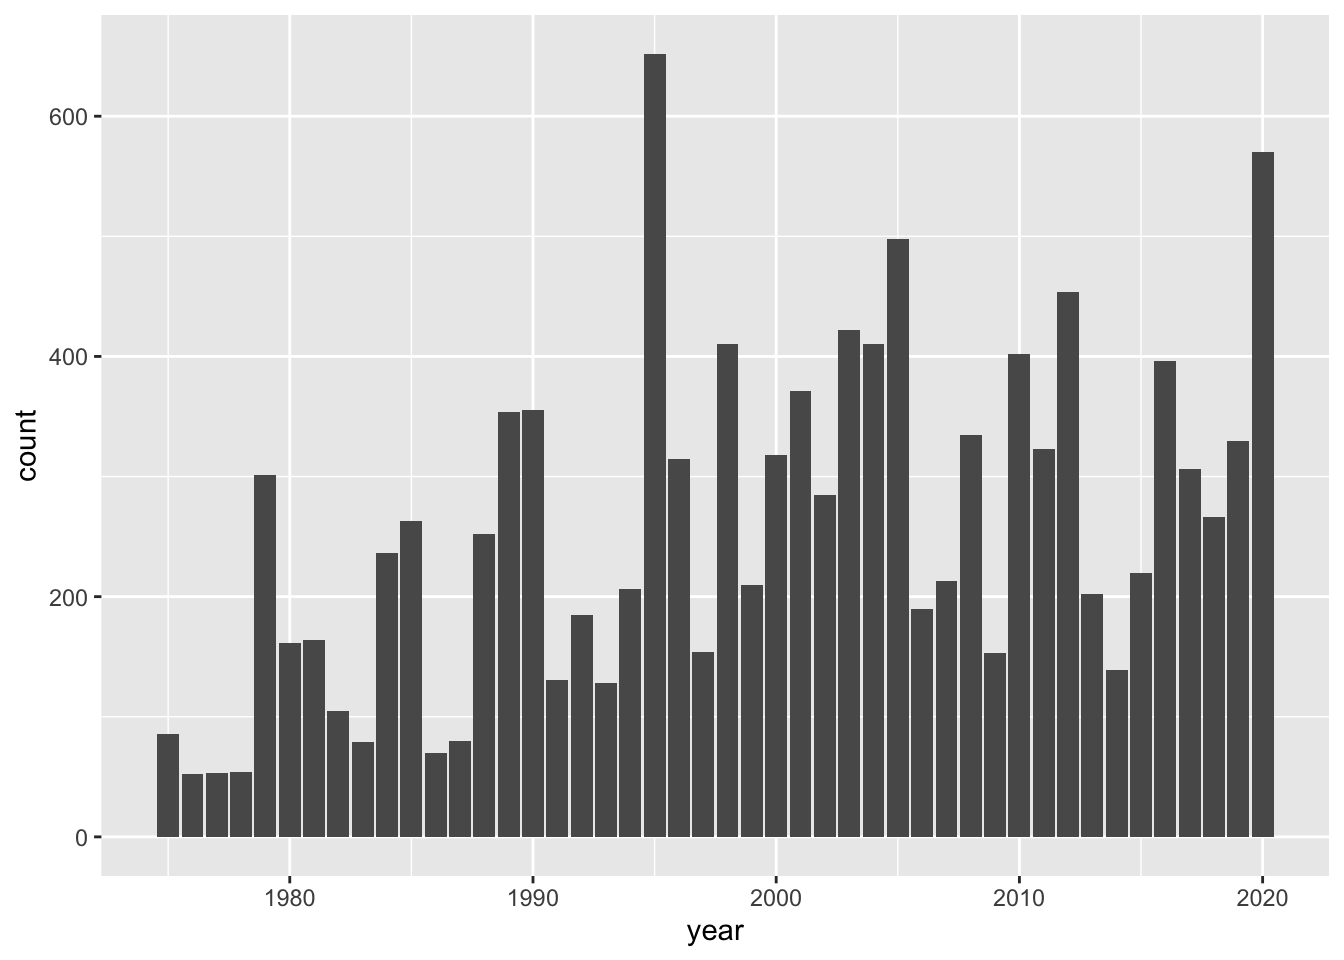
\includegraphics{R-tidy-hurricanes_files/figure-latex/unnamed-chunk-43-1.pdf}

We discovered that the 41-year period of recorded data from 1975 to 2015. We
can take a further step and ask: how many storms are there in each year?

To answer this question, we need to do some data manipulation with \texttt{"dplyr"}.
Our general recommendation when working with \texttt{"dplyr"}'s functions, especially
when you are learning about them, is to do computations step by step, deciding
which columns you need to use, which rows to consider, which functions to call,
and so on.

Think about the columns that we need to select to find the number of unique
storms per year. We obviously need \texttt{year}, but this column alone it's not enough
because for any given storm we have multiple records with the same year.
Therefore, we also need column \texttt{name}.

For illustration purposes, we are going to build the data manipulation pipeline
step by step. As you get more comfortable with \texttt{"dplyr"} and other functions,
you won't have the need to disect every single command.

A first step is to \texttt{select()} variables \texttt{year} and \texttt{name}:

\begin{Shaded}
\begin{Highlighting}[]
\FunctionTok{select}\NormalTok{(storms, year, name)}
\end{Highlighting}
\end{Shaded}

\begin{verbatim}
## # A tibble: 11,859 x 2
##     year name 
##    <dbl> <chr>
##  1  1975 Amy  
##  2  1975 Amy  
##  3  1975 Amy  
##  4  1975 Amy  
##  5  1975 Amy  
##  6  1975 Amy  
##  7  1975 Amy  
##  8  1975 Amy  
##  9  1975 Amy  
## 10  1975 Amy  
## # ... with 11,849 more rows
\end{verbatim}

Next, we need to \texttt{group\_by()} year. At first glance, the previous output and
the output below seem identical. But notice the tiny difference: the output
below has a second line of text with some relevant information:
\texttt{\#\ Groups:\ \ \ year\ {[}41{]}}, telling us that the values are grouped by year.

\begin{Shaded}
\begin{Highlighting}[]
\FunctionTok{group\_by}\NormalTok{(}\FunctionTok{select}\NormalTok{(storms, year, name), year)}
\end{Highlighting}
\end{Shaded}

\begin{verbatim}
## # A tibble: 11,859 x 2
## # Groups:   year [46]
##     year name 
##    <dbl> <chr>
##  1  1975 Amy  
##  2  1975 Amy  
##  3  1975 Amy  
##  4  1975 Amy  
##  5  1975 Amy  
##  6  1975 Amy  
##  7  1975 Amy  
##  8  1975 Amy  
##  9  1975 Amy  
## 10  1975 Amy  
## # ... with 11,849 more rows
\end{verbatim}

Then, we identify the \texttt{distinct()} values (combination of year-name):

\begin{Shaded}
\begin{Highlighting}[]
\FunctionTok{distinct}\NormalTok{(}\FunctionTok{group\_by}\NormalTok{(}\FunctionTok{select}\NormalTok{(storms, year, name), year))}
\end{Highlighting}
\end{Shaded}

\begin{verbatim}
## # A tibble: 512 x 2
## # Groups:   year [46]
##     year name    
##    <dbl> <chr>   
##  1  1975 Amy     
##  2  1975 Caroline
##  3  1975 Doris   
##  4  1976 Belle   
##  5  1976 Gloria  
##  6  1977 Anita   
##  7  1977 Clara   
##  8  1977 Evelyn  
##  9  1978 Amelia  
## 10  1978 Bess    
## # ... with 502 more rows
\end{verbatim}

For convenience purposes, let's assign this table into its own object,
which we can call \texttt{storms\_year\_name}

\begin{Shaded}
\begin{Highlighting}[]
\NormalTok{storms\_year\_name }\OtherTok{\textless{}{-}} \FunctionTok{distinct}\NormalTok{(}\FunctionTok{group\_by}\NormalTok{(}\FunctionTok{select}\NormalTok{(storms, year, name), year))}
\end{Highlighting}
\end{Shaded}

Finally, we need to \texttt{count()} how many storms are in each year:

\begin{Shaded}
\begin{Highlighting}[]
\FunctionTok{count}\NormalTok{(storms\_year\_name, year)}
\end{Highlighting}
\end{Shaded}

\begin{verbatim}
## # A tibble: 46 x 2
## # Groups:   year [46]
##     year     n
##    <dbl> <int>
##  1  1975     3
##  2  1976     2
##  3  1977     3
##  4  1978     4
##  5  1979     7
##  6  1980     8
##  7  1981     5
##  8  1982     5
##  9  1983     4
## 10  1984    10
## # ... with 36 more rows
\end{verbatim}

All the previous commands can be assembled together with various embedded lines
of code:

\begin{Shaded}
\begin{Highlighting}[]
\NormalTok{storms\_per\_year }\OtherTok{\textless{}{-}} \FunctionTok{count}\NormalTok{(}
  \FunctionTok{distinct}\NormalTok{(}
    \FunctionTok{group\_by}\NormalTok{(}
      \FunctionTok{select}\NormalTok{(storms, year, name), }
\NormalTok{      year)}
\NormalTok{    )}
\NormalTok{  )}

\NormalTok{storms\_per\_year}
\end{Highlighting}
\end{Shaded}

\begin{verbatim}
## # A tibble: 46 x 2
## # Groups:   year [46]
##     year     n
##    <dbl> <int>
##  1  1975     3
##  2  1976     2
##  3  1977     3
##  4  1978     4
##  5  1979     7
##  6  1980     8
##  7  1981     5
##  8  1982     5
##  9  1983     4
## 10  1984    10
## # ... with 36 more rows
\end{verbatim}

Now that we have the counts or frequencies, we can make our next barchart.
In this case, we will use the table \texttt{storms\_year\_name} as the input data for
\texttt{ggplot()}:

\begin{Shaded}
\begin{Highlighting}[]
\FunctionTok{ggplot}\NormalTok{(}\AttributeTok{data =}\NormalTok{ storms\_year\_name) }\SpecialCharTok{+} 
  \FunctionTok{geom\_bar}\NormalTok{(}\FunctionTok{aes}\NormalTok{(}\AttributeTok{x =}\NormalTok{ year))}
\end{Highlighting}
\end{Shaded}

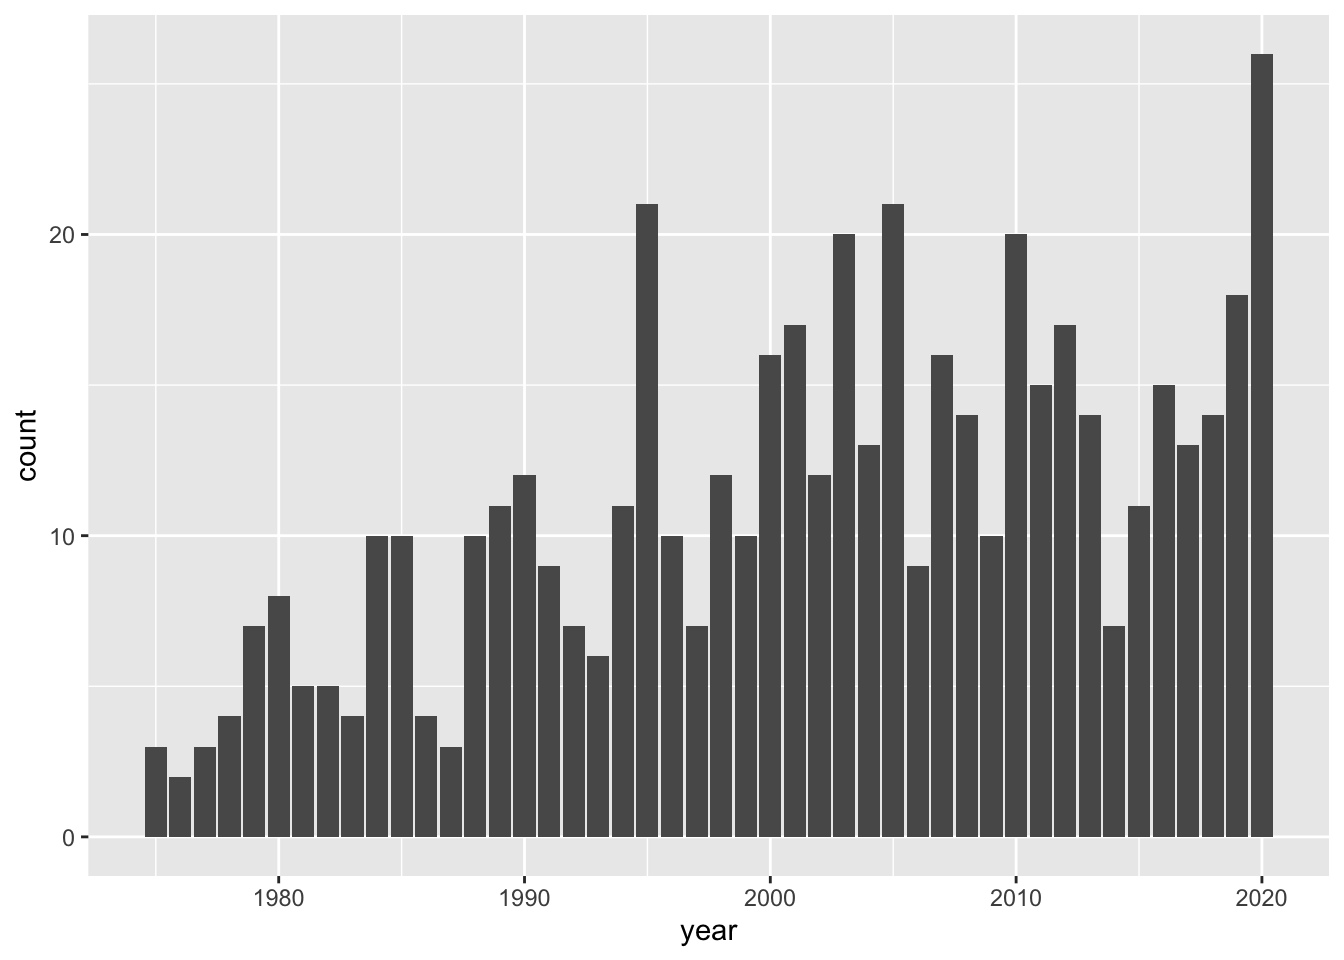
\includegraphics{R-tidy-hurricanes_files/figure-latex/unnamed-chunk-50-1.pdf}

By looking at the chart, there are some fairly tall bars. Although it's hard
to see exactly which years have a considerably large number of storms,
eyeballing things out it seems that around 1995, 2003, 2005, and 2010 there are
20 or more storms. We can find the actual answer by using \texttt{arrange()},
specifying the counts to be shown in descending order---with \texttt{desc()}:

\begin{Shaded}
\begin{Highlighting}[]
\FunctionTok{arrange}\NormalTok{(storms\_per\_year, }\FunctionTok{desc}\NormalTok{(n))}
\end{Highlighting}
\end{Shaded}

\begin{verbatim}
## # A tibble: 46 x 2
## # Groups:   year [46]
##     year     n
##    <dbl> <int>
##  1  2020    26
##  2  1995    21
##  3  2005    21
##  4  2003    20
##  5  2010    20
##  6  2019    18
##  7  2001    17
##  8  2012    17
##  9  2000    16
## 10  2007    16
## # ... with 36 more rows
\end{verbatim}

As you can tell, in the 41-year period from 1975 to 2015, there are two years,
1995 and 2005, with a maximum number of storms equal to 21.

\begin{center}\rule{0.5\linewidth}{0.5pt}\end{center}

\hypertarget{your-turn-3}{%
\section{Your Turn}\label{your-turn-3}}

\begin{itemize}
\item
  Use \texttt{"dplyr"} functions/commands to create a table (e.g.~tibble)
  \texttt{storm\_records\_per\_year} containing three columns: 1) \texttt{name} of storm, 2) \texttt{year}
  of storm, and 3) \texttt{count} for number of recorded valued (of the corresponding
  storm).
\item
  Use \texttt{"dplyr"} functions/commands to create a table (e.g.~tibble)
  \texttt{storms\_categ5} containing the name and year of those storms of category 5.
\item
  Use \texttt{"dplyr"} functions/commands to display a table showing the \texttt{status},
  \texttt{avg\_pressure} (average pressure), and \texttt{avg\_wind} (average wind speed), for
  each type of storm \texttt{category}. This table should contain four columns: 1)
  \texttt{category}, 2) \texttt{status}, 3) \texttt{avg\_pressure}, and 4) \texttt{avg\_wind}.
\item
  Use \texttt{"dplyr"} functions/commands to create a table (e.g.~tibble)
  \texttt{max\_wind\_per\_storm} containing three columns: 1) \texttt{year} of storm, 2) \texttt{name} of
  storm, and 3) \texttt{max\_wind} maximum wind speed record (for that storm).
\item
  Use \texttt{"dplyr"} functions/commands to create a table (e.g.~tibble)
  \texttt{max\_wind\_per\_year} containing three columns: 1) \texttt{year} of storm, 2) \texttt{name} of
  storm, and 3) \texttt{wind} maximum wind speed record (for that year). Arrange rows by
  wind speed in decreasing order.
\end{itemize}

  \bibliography{book.bib}

\end{document}
